
%A280.TSP
\subsubsection{a280.TSP}
\begin{table}[hbtp]
    \centering
    \caption{Experimento con el problema a280.TSP.}    
    \small
    \begin{tabular}{| l   l | r | r | r |   }
    \hline\multicolumn{5}{|c|}{ \rowcolor[gray]{0.8}a280.TSP} \\\hline
    \multicolumn{2}{|l|}{Resultado Original : 3418}   & Promedio & Mejor & Peor \\ 
                \hline
                & Recocido  &  3364.17 & 3329 & \cellcolor[gray]{0.9} 3394  \\ 
Con cuadrantes  & Greedy    &  3363.79 & 3335 & 3396  \\ 
                & Genético  & \cellcolor[gray]{0.9} 3354.06 & \cellcolor[gray]{0.9} 3318 & 3418 \\ 
                    \hline
                & Recocido  &  5078.51 & \cellcolor[gray]{0.9} 4711 & 5345   \\ 
Sin cuadrantes  & Greedy    &  5101.88 & 4804 & 5410   \\ 
                & Genético  &  \cellcolor[gray]{0.9} 4876.34 & 4747 & \cellcolor[gray]{0.9} 5066 \\ 
                    \hline
    \end{tabular}
    \label{table:EXP_a280.TSP}
\end{table}
 \begin{figure}[hbtp]
    \centering
        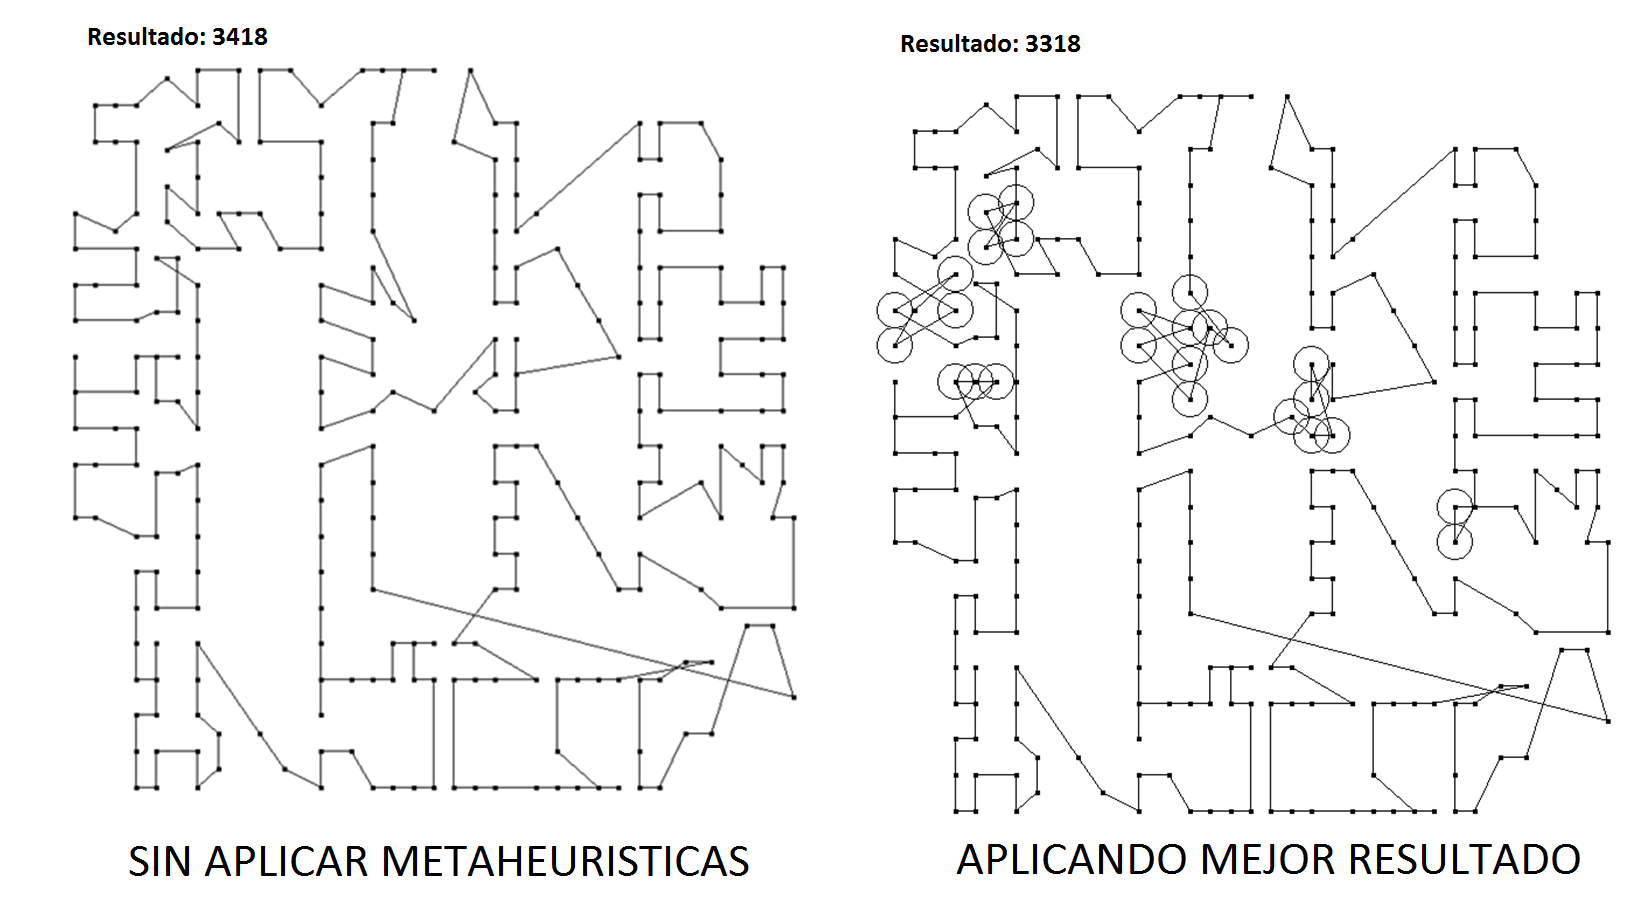
\includegraphics[width=1\textwidth]{PruebasResultados/Experimentos_Comparativas/a280.png}
        \caption{Comparativa a280.tsp.}
        \label{fig:a280_comparativa.png}
\end{figure}
 \begin{figure}[hbtp]
    \centering
        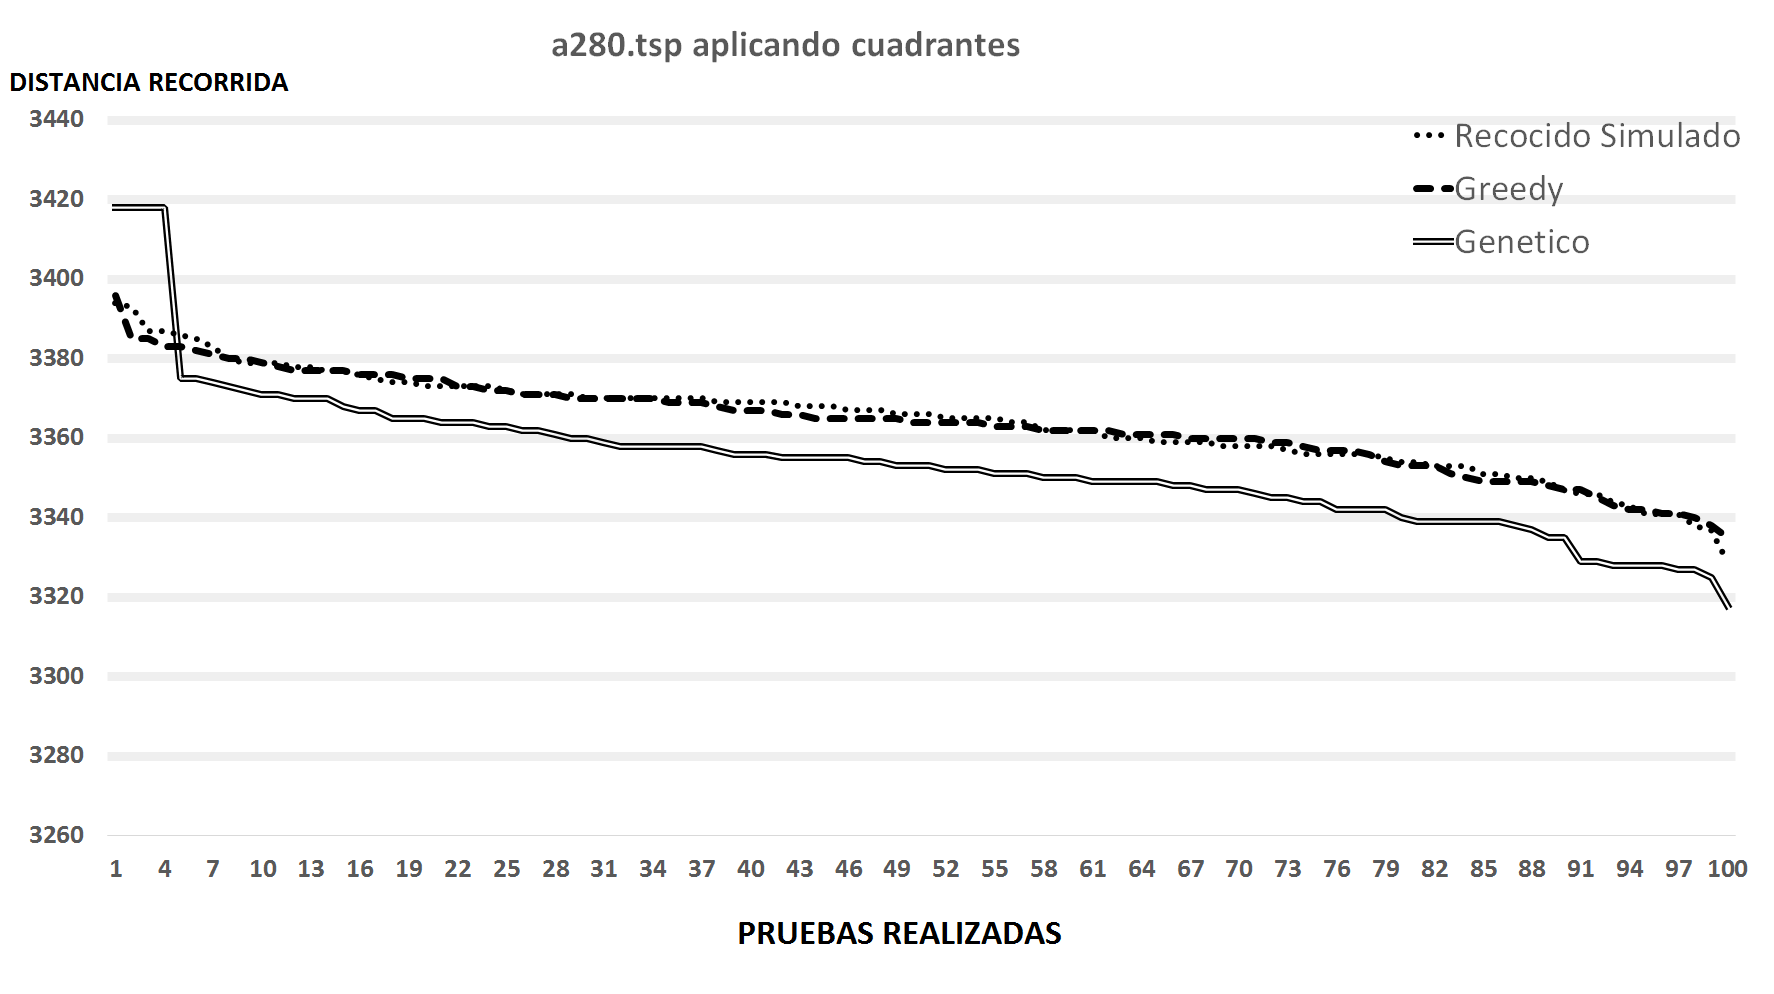
\includegraphics[width=1\textwidth]{PruebasResultados/Experimentos_Graficos_Con/a280.png}
        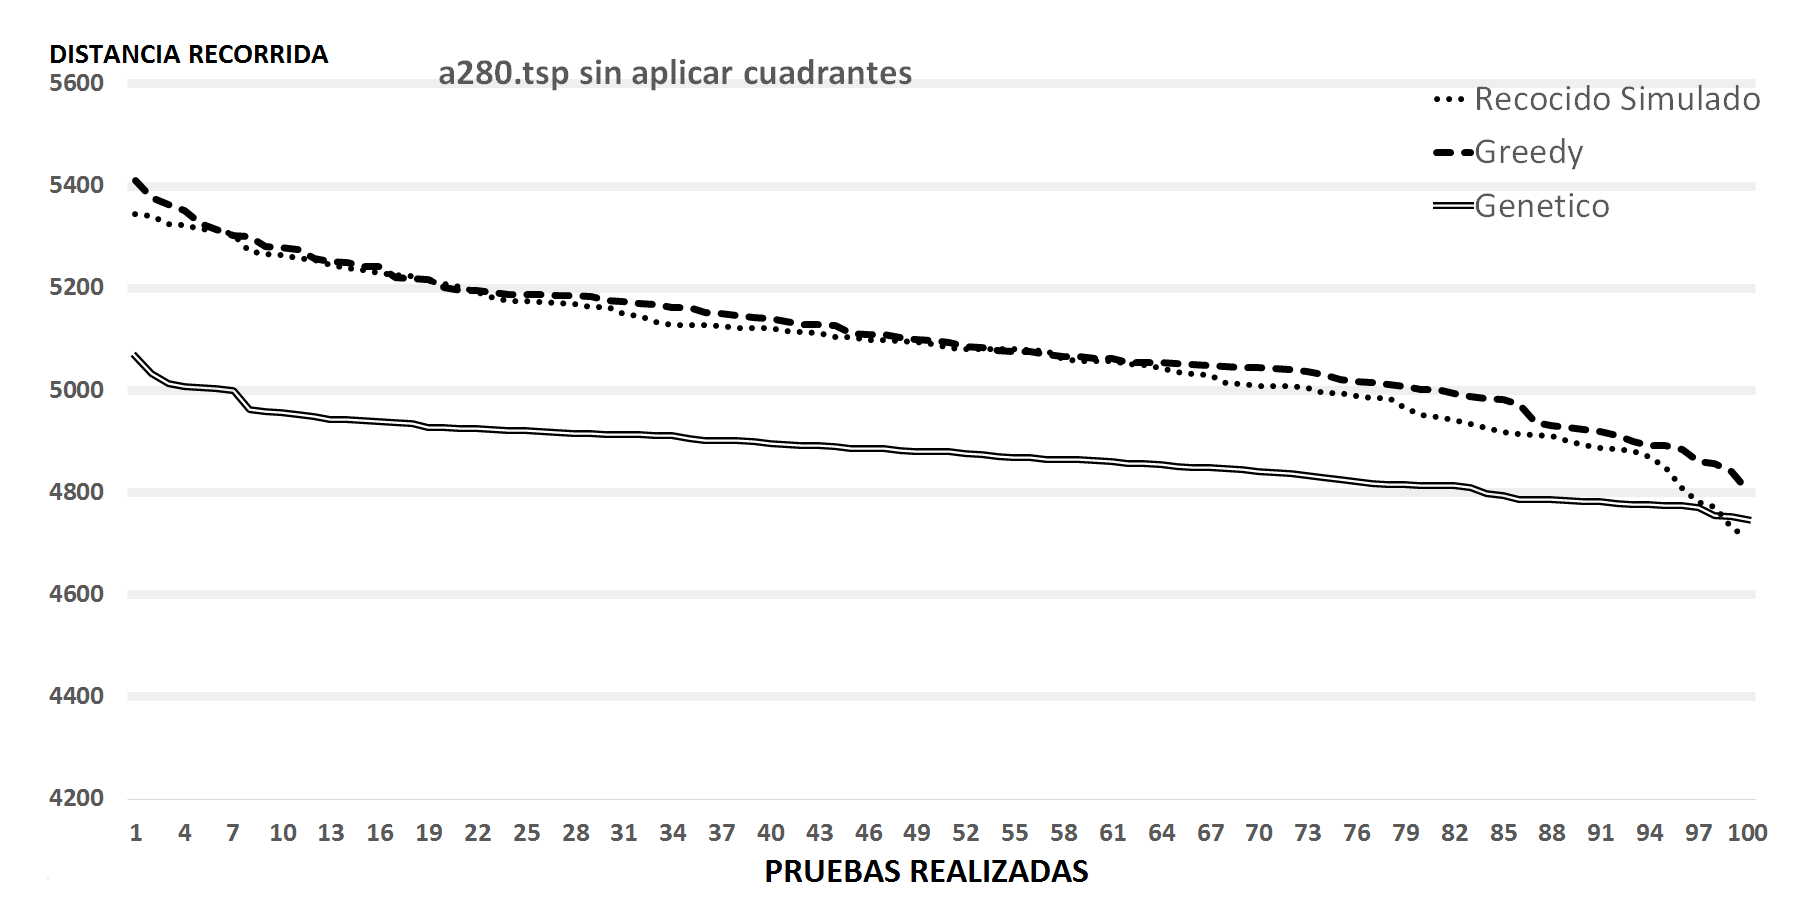
\includegraphics[width=1\textwidth]{PruebasResultados/Experimentos_Graficos_Sin/a280.png}
        \caption{Gráficos a280.tsp con cuadrantes y sin cuadrantes.}
        \label{fig:a280_grafica.png}
\end{figure}
\newpage

\hspace*{1cm}Como se puede observar en la figura \ref{fig:a280_explicado.png}, los círculos marcan las zonas mutadas de la solución obtenida mediante el método de cuadrantes. En la figura \ref{fig:a280_comparativa.png} algunos puntos que se muestran en la imagen de la derecha están encerrados en círculos, estos puntos están marcados así porque fueron colocados fuera de la posición original que se le asignó por el método de cuadrantes.\\
\hspace*{1cm}Regresando a la figura \ref{fig:a280_explicado.png} se puede ver 3 imágenes:
\begin{itemize}
    \item \textbf{A: }Es el problema resuelto por el método de cuadrantes.
    \item \textbf{B: }El mismo problema, solo que fue modificado usando metaheurísticas, aquí se puede apreciar que varios puntos fueron encerrados en círculos ya comentando su funcionalidad 
    \item \textbf{C: }Es la imagen B sin los puntos marcados, para que se puede apreciar con mejor detalle las diferencias que tiene con la imagen A.
\end{itemize}

\begin{figure}[hbtp]
    \centering
        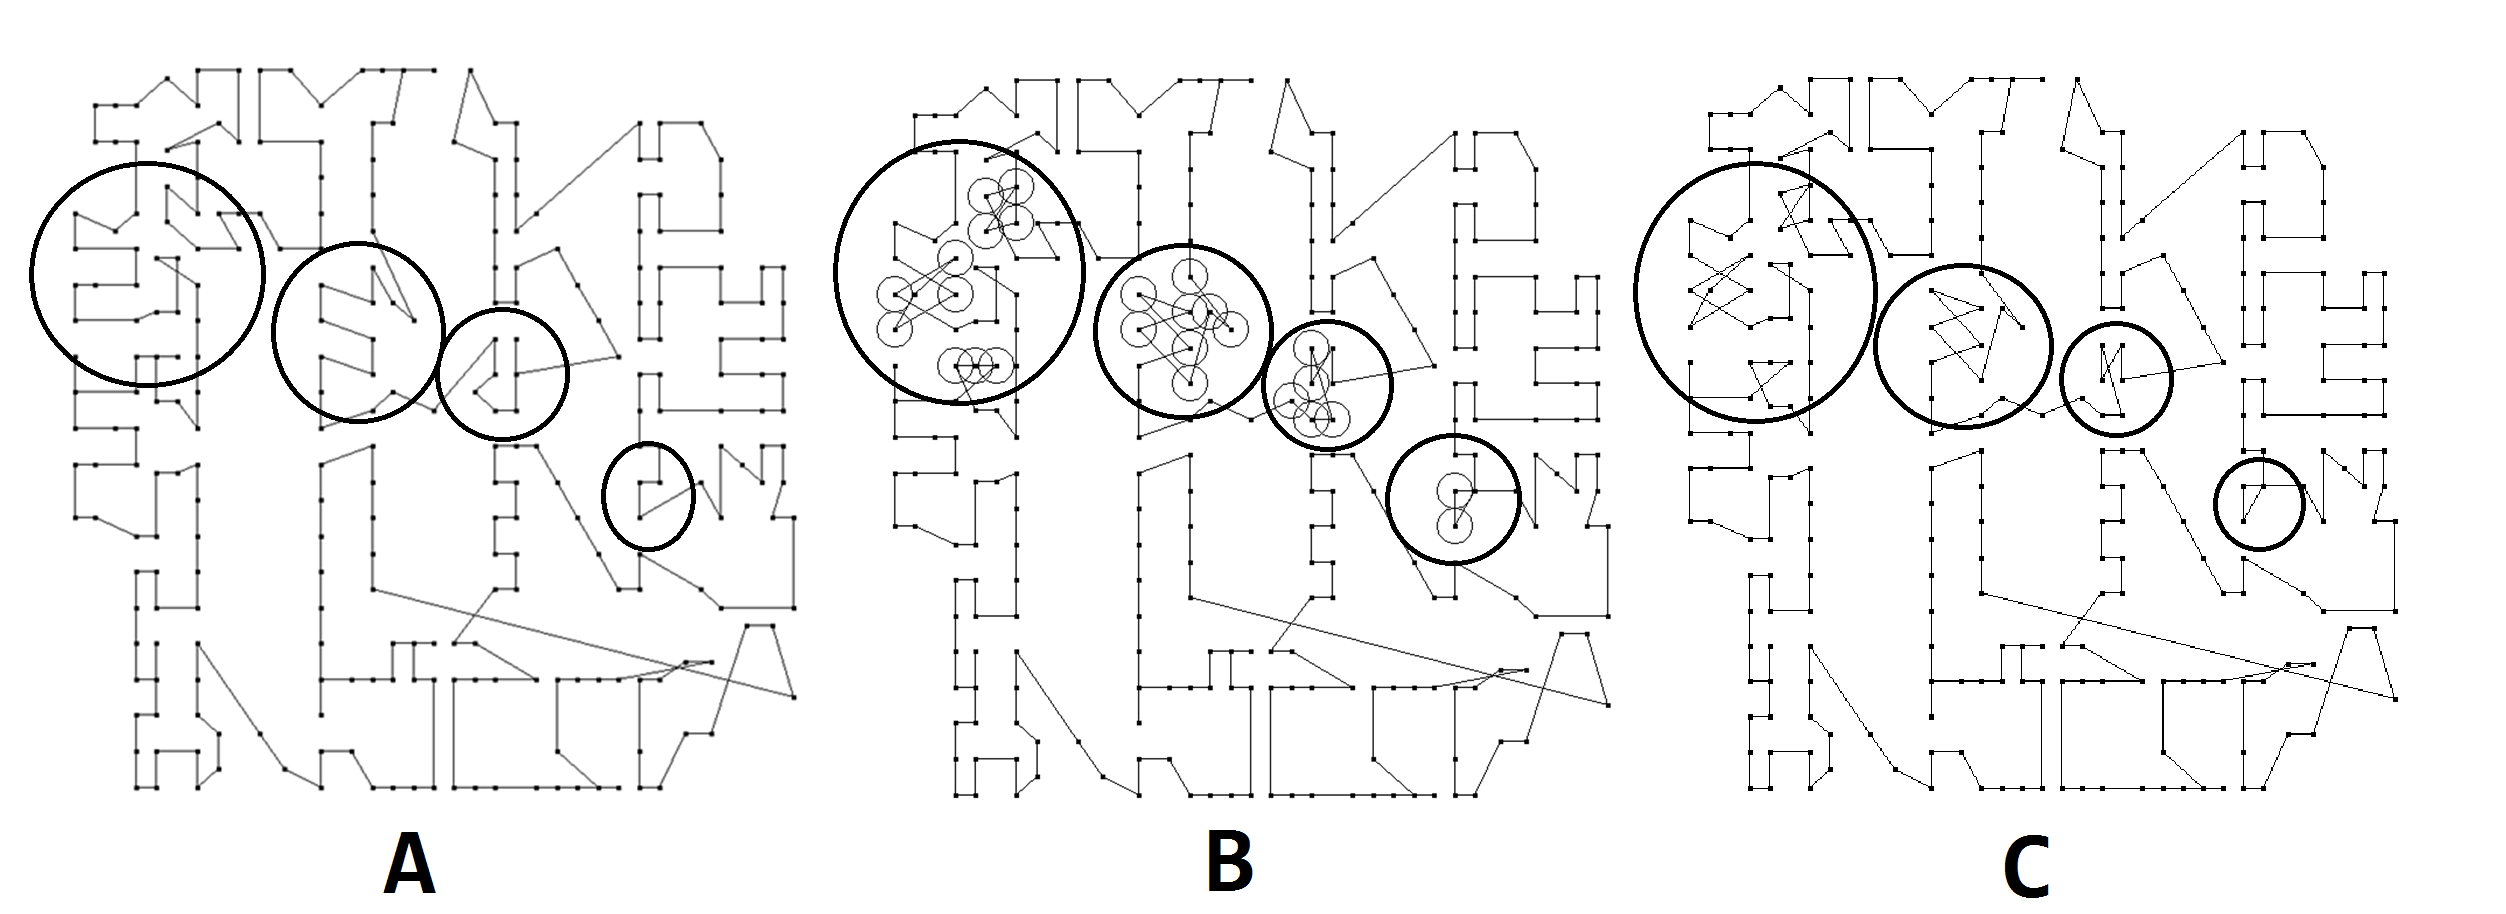
\includegraphics[width=1\textwidth]{PruebasResultados/Imagenes/a280_explicado.png}
        \caption{Explicación de los cambios realizados en el a280.tsp.}
        \label{fig:a280_explicado.png}
\end{figure}

\hspace*{1cm}Ya conociendo para que sirve esta imagen se procederá con los demás experimentos.

\newpage

%brd14051.TSP
\subsubsection{brd14051.TSP}
\begin{table}[hbtp]
    \centering 
    \caption{Experimento con el problema brd14051.tsp.}    
	\begin{tabular}{ | l   l | r | r | r |   }
    \hline\multicolumn{5}{|c|}{ \rowcolor[gray]{0.8}brd14051.tsp} \\\hline
    \multicolumn{2}{|l|}{Resultado Original :623324}  & Promedio & Mejor & Peor \\ 
                \hline
                & Recocido  & \cellcolor[gray]{0.9} 619876.89 & \cellcolor[gray]{0.9} 618878 & \cellcolor[gray]{0.9} 620546 \\ 
 Con cuadrantes & Greedy    & 619899.03 & 619060 & 620743  \\ 
                & Genético  & 621842.30 & 621273 & 622688  \\ 
                \hline
                & Recocido  & 13091307.46 & \cellcolor[gray]{0.9} 12612710 & 13458979 \\ 
 Sin cuadrantes & Greedy    & \cellcolor[gray]{0.9} 13071094.56 & 12811921 & \cellcolor[gray]{0.9} 13411800 \\ 
                & Genético  & 23478563.40 & 23433764 & 23520252 \\ 
                \hline
    \end{tabular}
    \label{table:EXP_brd14051.tsp}
\end{table}
\begin{figure}[hbtp]
    \centering
        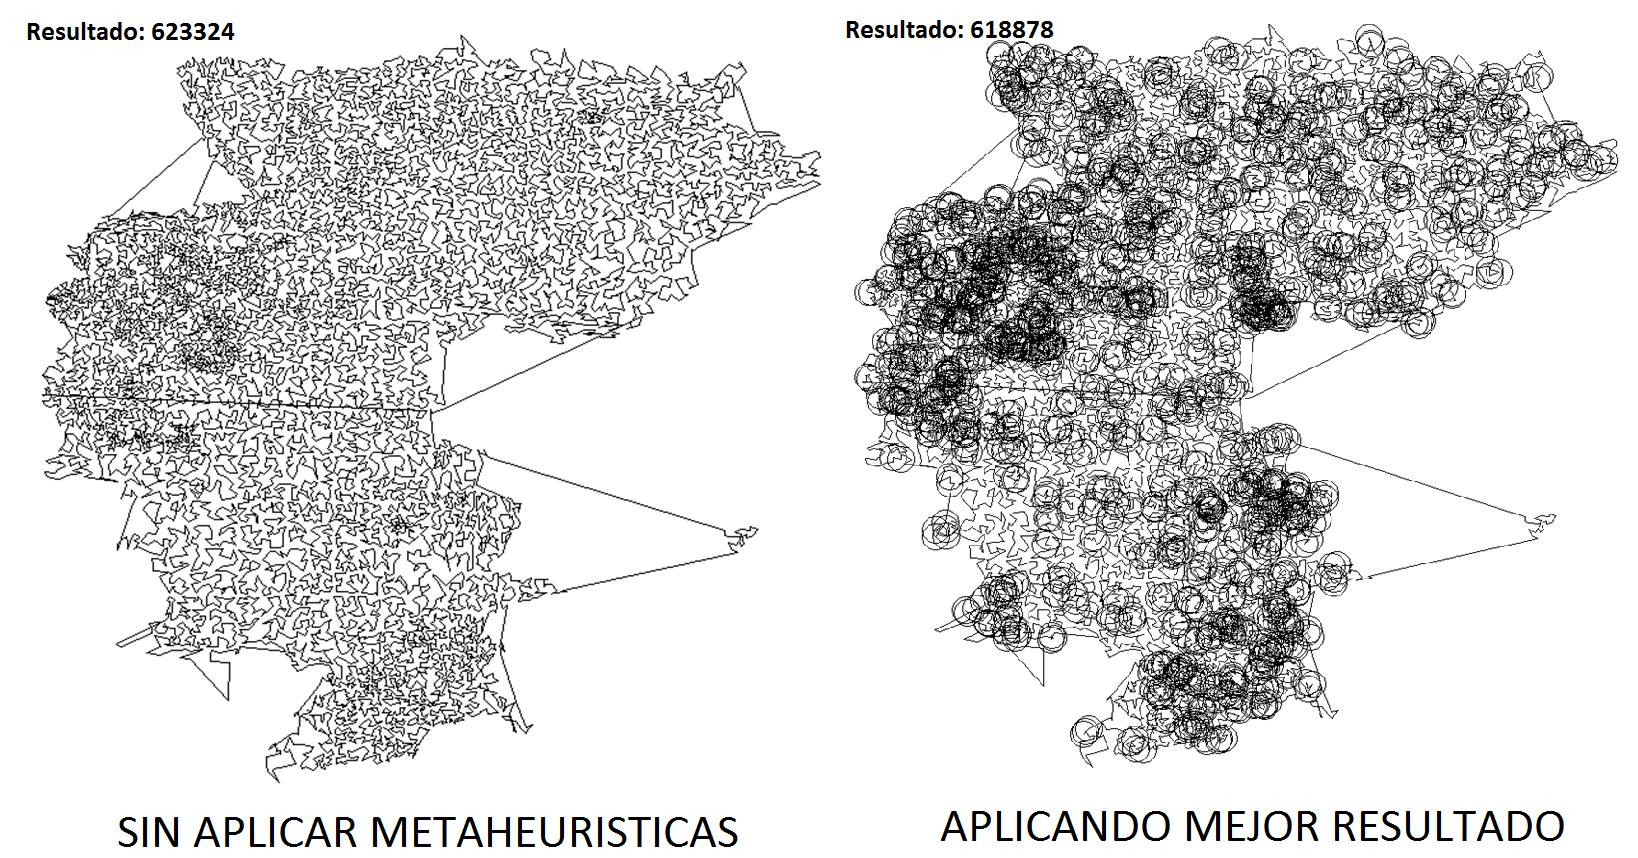
\includegraphics[width=1\textwidth]{PruebasResultados/Experimentos_Comparativas/brd14051.png}
        \caption{Comparativa brd14051.tsp.}
        \label{fig:brd14051_comparativa.png}
\end{figure}
 \begin{figure}[hbtp]
    \centering
        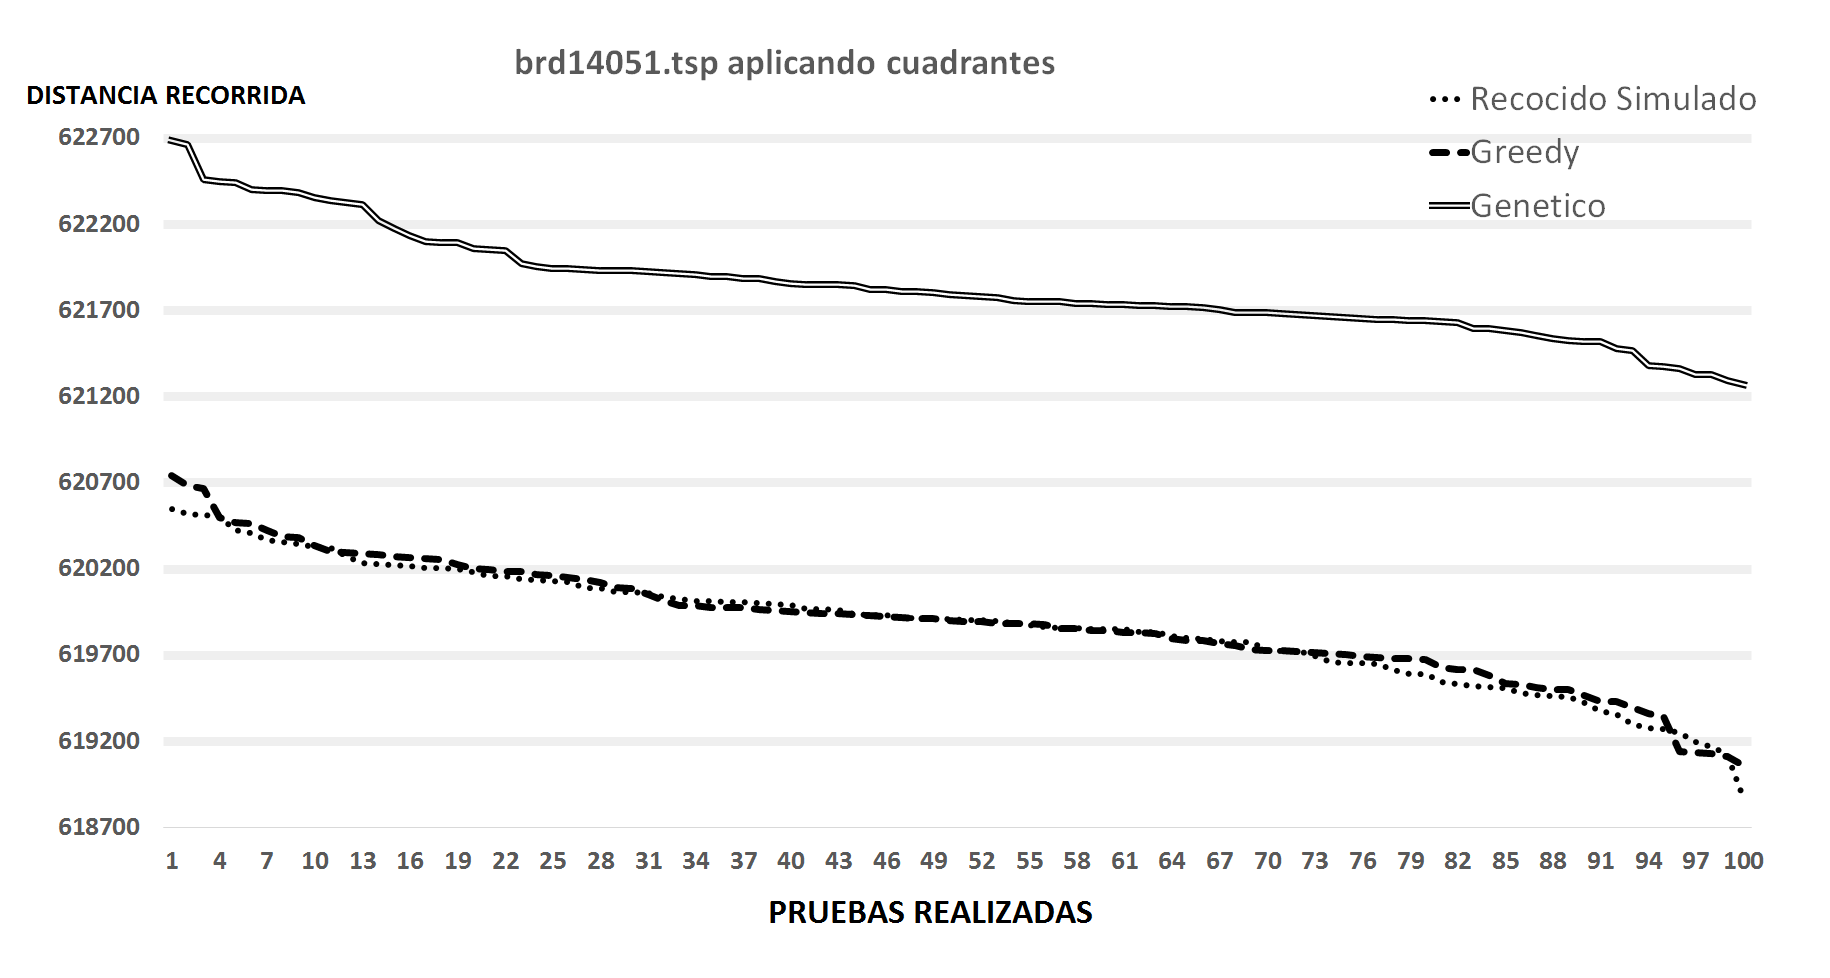
\includegraphics[width=1\textwidth]{PruebasResultados/Experimentos_Graficos_Con/brd14051.png}
        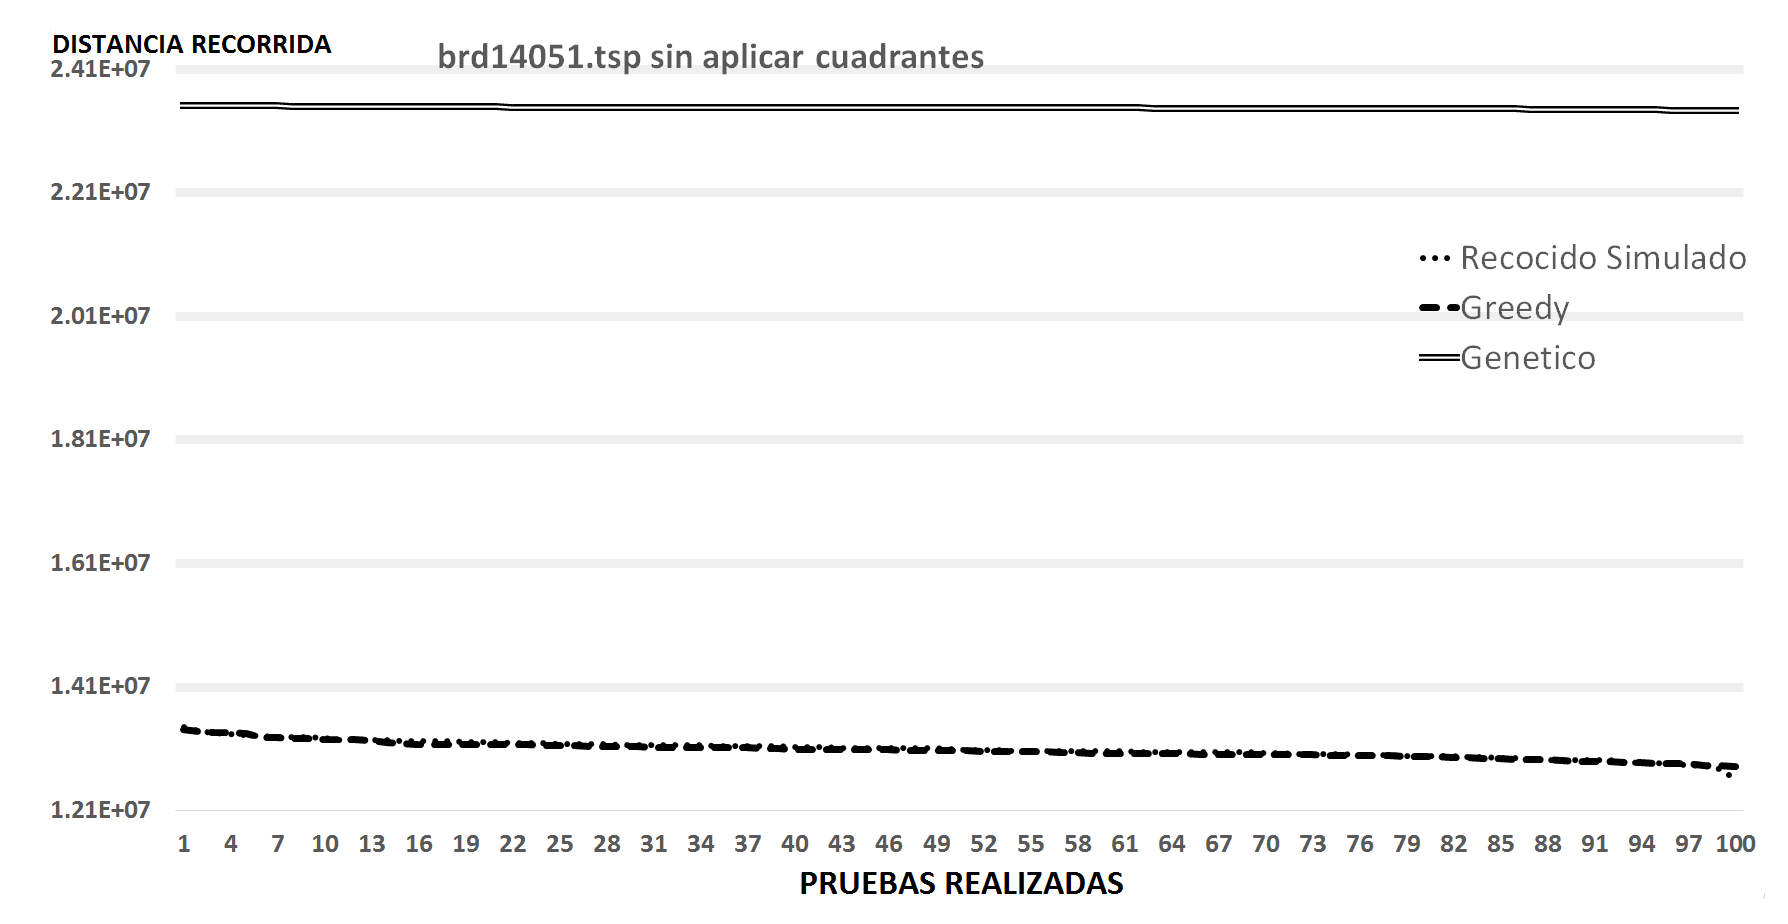
\includegraphics[width=1\textwidth]{PruebasResultados/Experimentos_Graficos_Sin/brd14051.png}
        \caption{Gráficos brd14051.tsp con cuadrantes y sin cuadrantes.}         
        \label{fig:brd14051_grafica.png} 
\end{figure}
\newpage

%CH150.TSP
\subsubsection{ch150.TSP}
\begin{table}[hbtp]
 \centering	
    \caption{Experimento con el problema ch150.tsp.} 
	\begin{tabular}{ | l   l | r | r | r |   }
         \hline\multicolumn{5}{|c|}{ \rowcolor[gray]{0.8} ch150.tsp } \\\hline
         \multicolumn{2}{|l|}{Resultado Original : 8579}   & Promedio & Mejor & Peor \\ 
                \hline
                & Recocido  &  8445.98 & 8272 & 8535  \\ 
 Con cuadrantes & Greedy    &  8446.02 & 8315 & 8540  \\ 
                & Genético  & \cellcolor[gray]{0.9}8358.81 & \cellcolor[gray]{0.9}8231 & \cellcolor[gray]{0.9}8427 \\ 
                \hline
                & Recocido  & \cellcolor[gray]{0.9} 26500.85 & 23162 & \cellcolor[gray]{0.9} 28674 \\ 
 Sin cuadrantes & Greedy    &  26614.55 & \cellcolor[gray]{0.9} 22417 & 29187 \\ 
                & Genético  &  34548.11 & 32091 & 37844 \\ 
                \hline
    \end{tabular}
    \label{table:EXP_ch150.tsp}
\end{table}
\begin{figure}[hbtp]
    \centering
        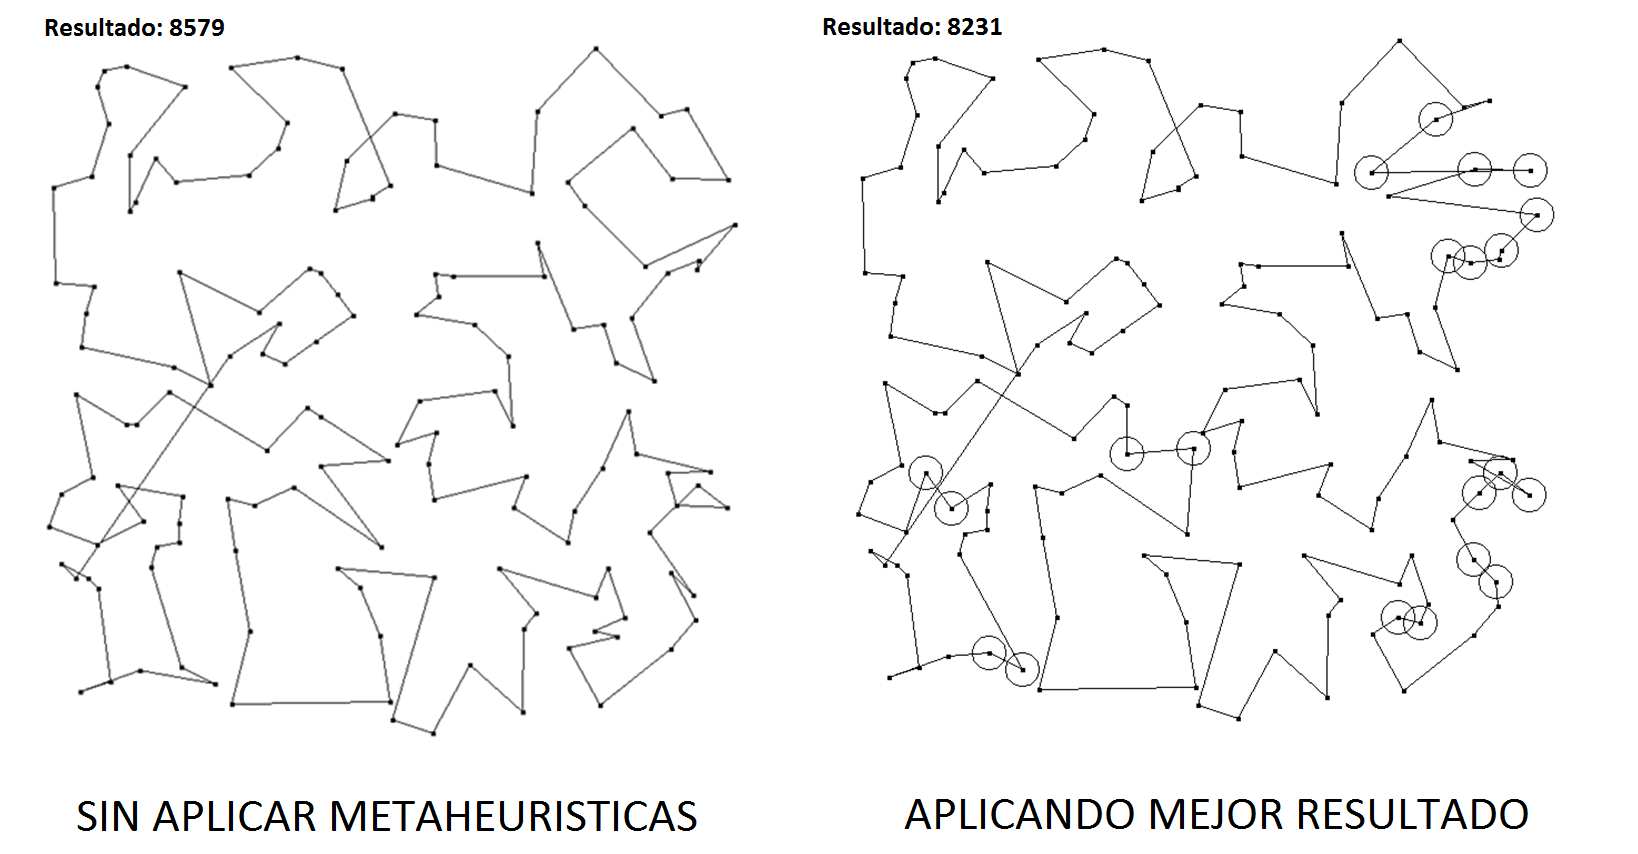
\includegraphics[width=1\textwidth]{PruebasResultados/Experimentos_Comparativas/ch150.png}
        \caption{Comparativa ch150.tsp.}
        \label{fig:ch150_comparativa.png}
\end{figure}
 \begin{figure}[hbtp]
    \centering
        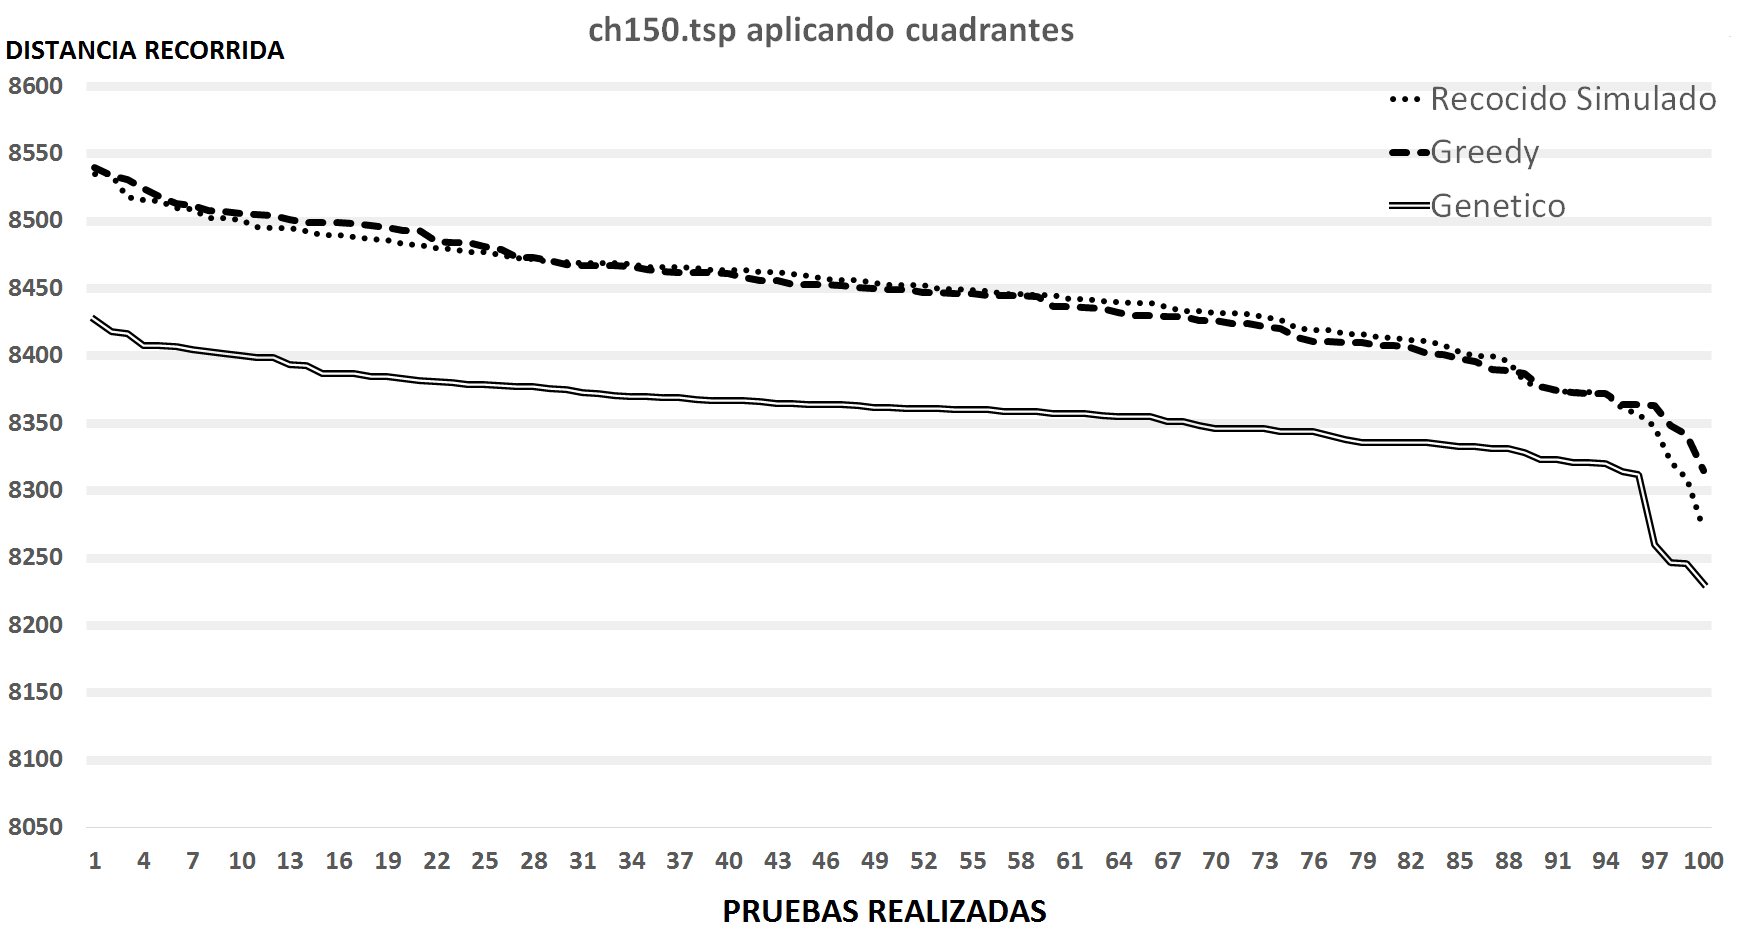
\includegraphics[width=1\textwidth]{PruebasResultados/Experimentos_Graficos_Con/ch150.png}
        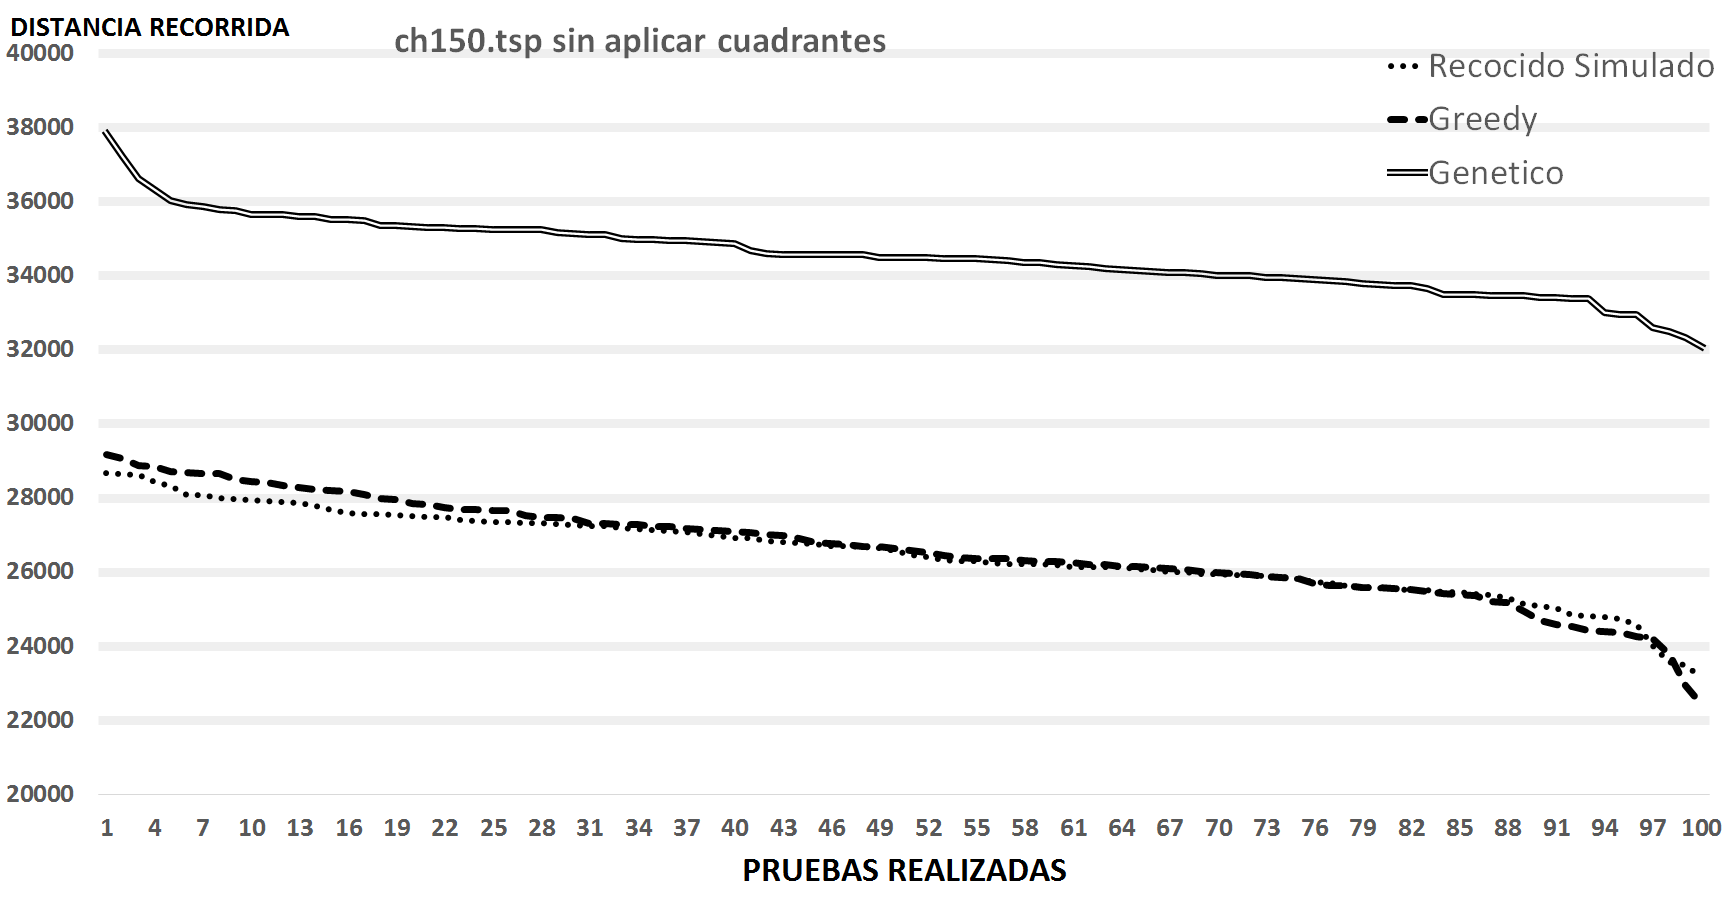
\includegraphics[width=1\textwidth]{PruebasResultados/Experimentos_Graficos_Sin/ch150.png}
        \caption{Gráficos ch150.tsp con cuadrantes y sin cuadrantes.}
        \label{fig:ch150_grafica.png}
\end{figure}
\newpage

%d1655.TSP
\subsubsection{d1655.TSP}
\begin{table}[hbtp]
 \centering 
    \caption{Experimento con el problema d1655.tsp.} 
	\begin{tabular}{ | l   l | r | r | r |   }
         \hline\multicolumn{5}{|c|}{ \rowcolor[gray]{0.8}d1655.tsp} \\ \hline
         \multicolumn{2}{|l|}{Resultado Original :83605}  & Promedio & Mejor & Peor \\ 
                \hline
                & Recocido  & 82500.78 & 82098 & 82881 \\ 
 Con cuadrantes & Greedy    & 82489.63 & 82014 & 82839 \\ 
                & Genético  & \cellcolor[gray]{0.9} 82244 & \cellcolor[gray]{0.9} 81996 & \cellcolor[gray]{0.9} 82447 \\ 
                \hline
                & Recocido  & 235605.87 & \cellcolor[gray]{0.9} 222473 & \cellcolor[gray]{0.9} 243750 \\ 
 Sin cuadrantes & Greedy    & 236306.2 & 226740 & 246172 \\ 
                & Genético  & \cellcolor[gray]{0.9} 264556.11 & 262348 & 266415 \\ 
                \hline
    \end{tabular}
    \label{table:EXP_d1655.tsp}
\end{table}
\begin{figure}[hbtp]
    \centering
        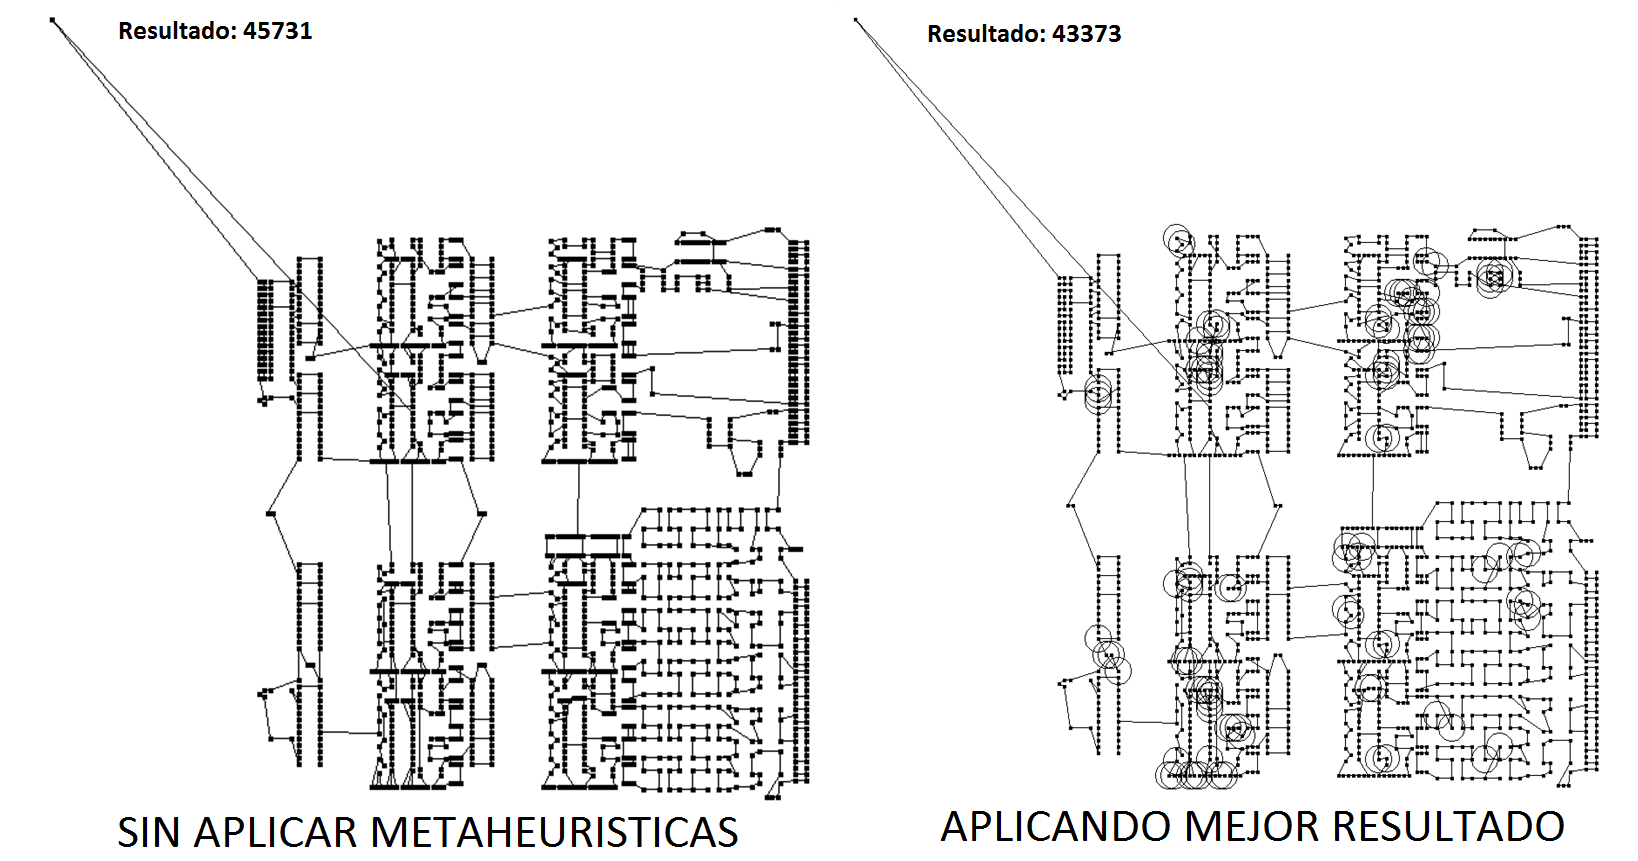
\includegraphics[width=1\textwidth]{PruebasResultados/Experimentos_Comparativas/d1655.png}
        \caption{Comparativa d1655.tsp.}
        \label{fig:d1655_comparativa.png}
\end{figure}
 \begin{figure}[hbtp]
    \centering
        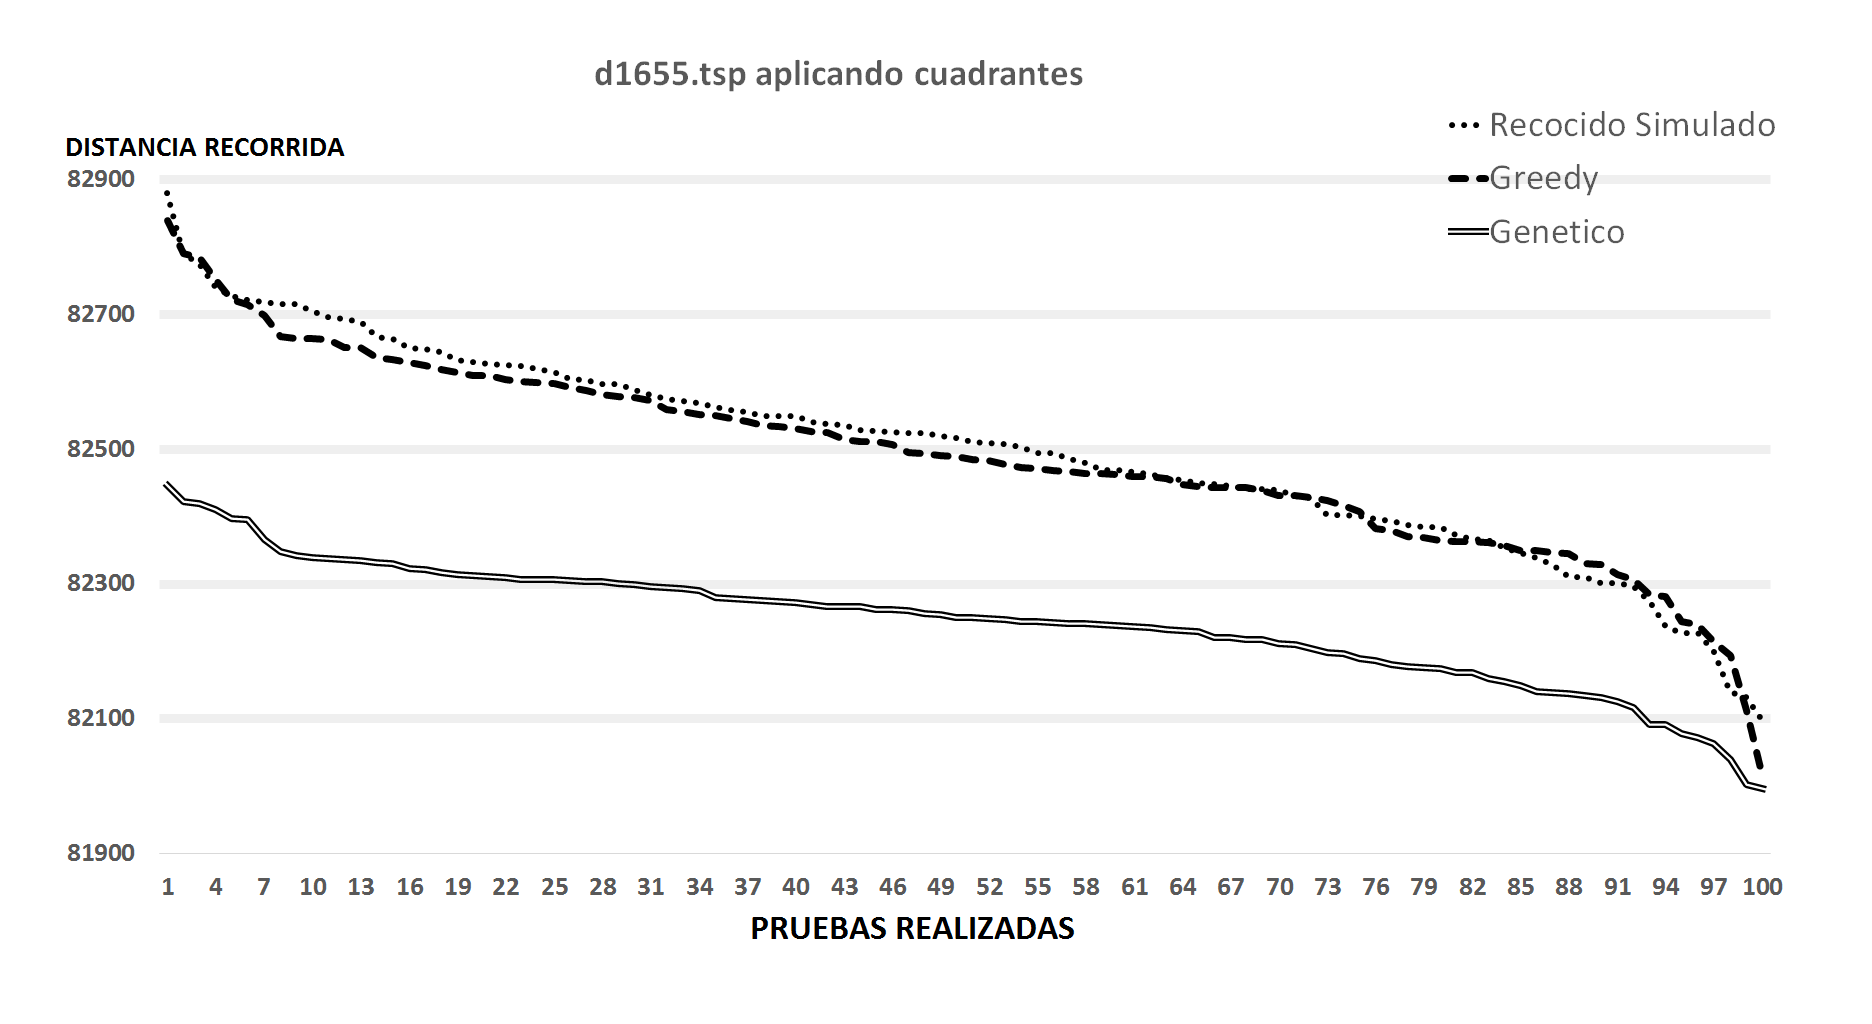
\includegraphics[width=1\textwidth]{PruebasResultados/Experimentos_Graficos_Con/d1655.png}
        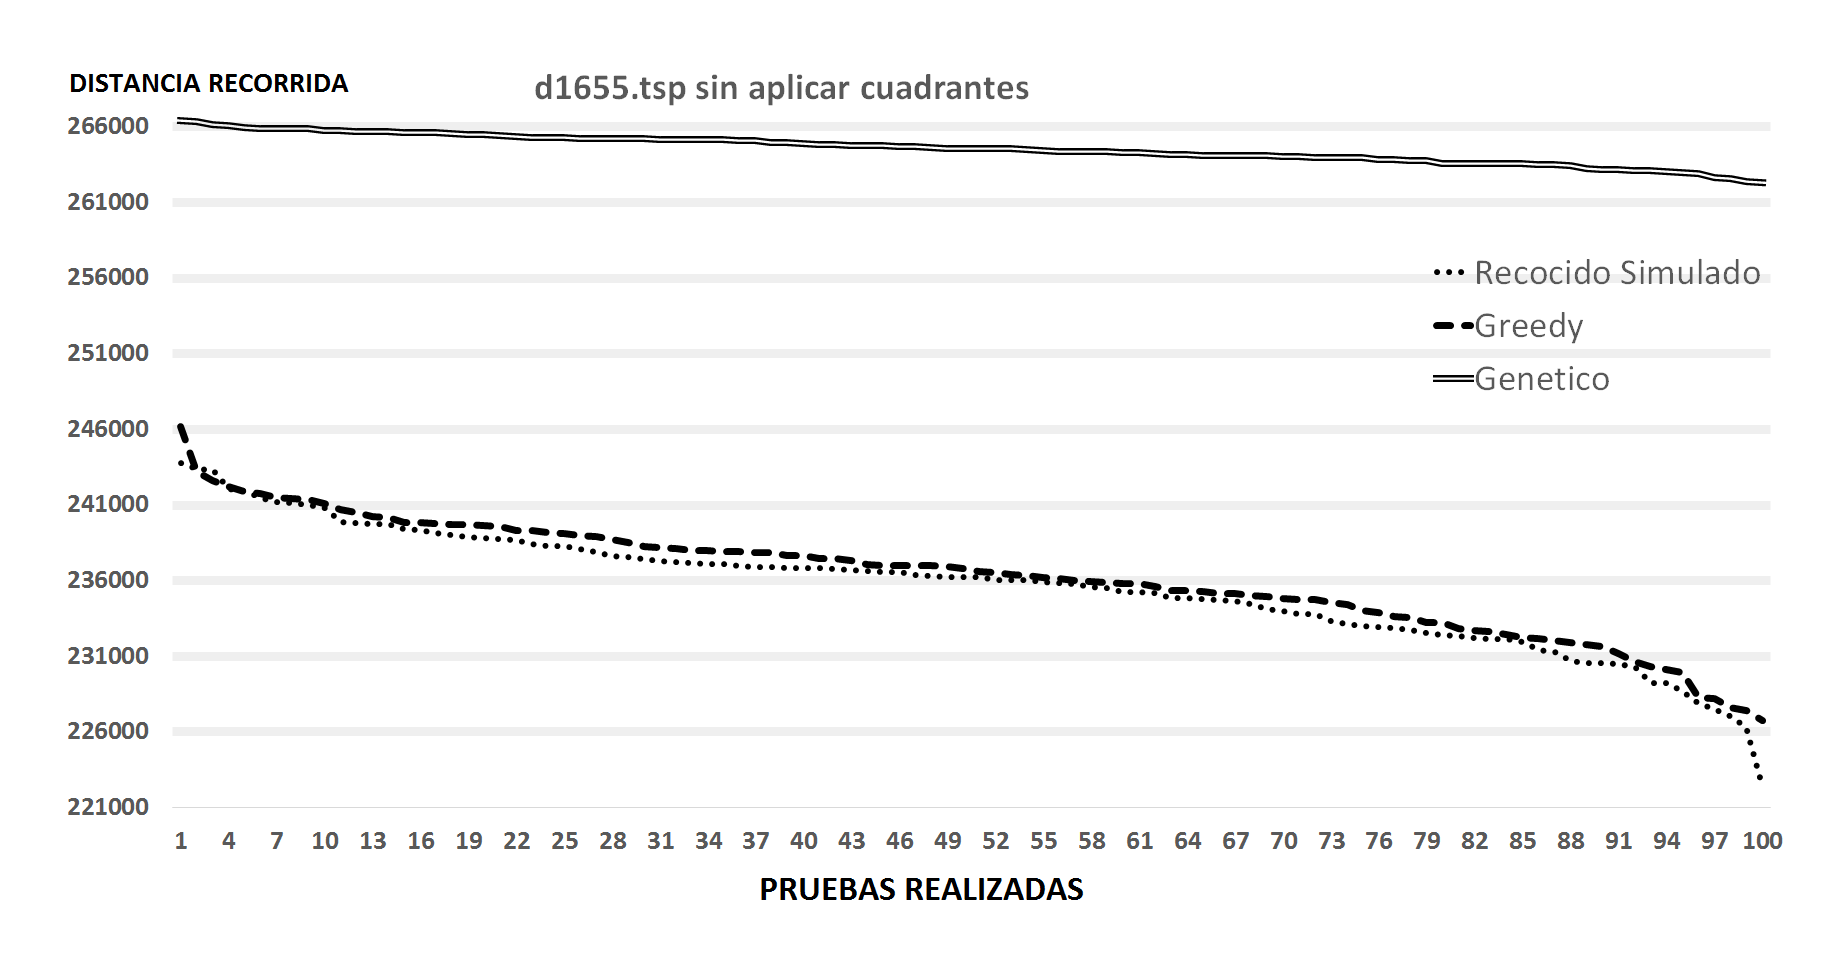
\includegraphics[width=1\textwidth]{PruebasResultados/Experimentos_Graficos_Sin/d1655.png}
        \caption{Gráficos d1655.tsp con cuadrantes y sin cuadrantes.}
        \label{fig:d1655_grafica.png}
\end{figure}
\newpage

%D493.TSP
\subsubsection{d493.TSP}
\begin{table}[hbtp]
 \centering 
    \caption{Experimento con el problema d493.tsp.}
	\begin{tabular}{ | l   l | r | r | r |   }
        \hline\multicolumn{5}{|c|}{ \rowcolor[gray]{0.8} d493.tsp} \\ \hline
        \multicolumn{2}{|l|}{Resultado Original : 45731} & Promedio & Mejor & Peor \\ 
                \hline
                & Recocido  & 44582.69 & 44124 & 45012  \\ 
 Con cuadrantes & Greedy    & 44604.21 & 44054 & 45275  \\ 
                & Genético  & \cellcolor[gray]{0.9} 43987.43 & \cellcolor[gray]{0.9} 43373 & \cellcolor[gray]{0.9} 44918  \\ 
                \hline
                & Recocido  & 96827.13 & 91468 & 102751   \\ 
 Sin cuadrantes & Greedy    & \cellcolor[gray]{0.9} 96002.89 & \cellcolor[gray]{0.9} 89956 & \cellcolor[gray]{0.9} 100955   \\ 
                & Genético  & 121326.2 & 115991 & 124989    \\ 
                \hline
    \end{tabular}
    \label{table:EXP_d493.tsp}
\end{table}
\begin{figure}[hbtp]
    \centering
        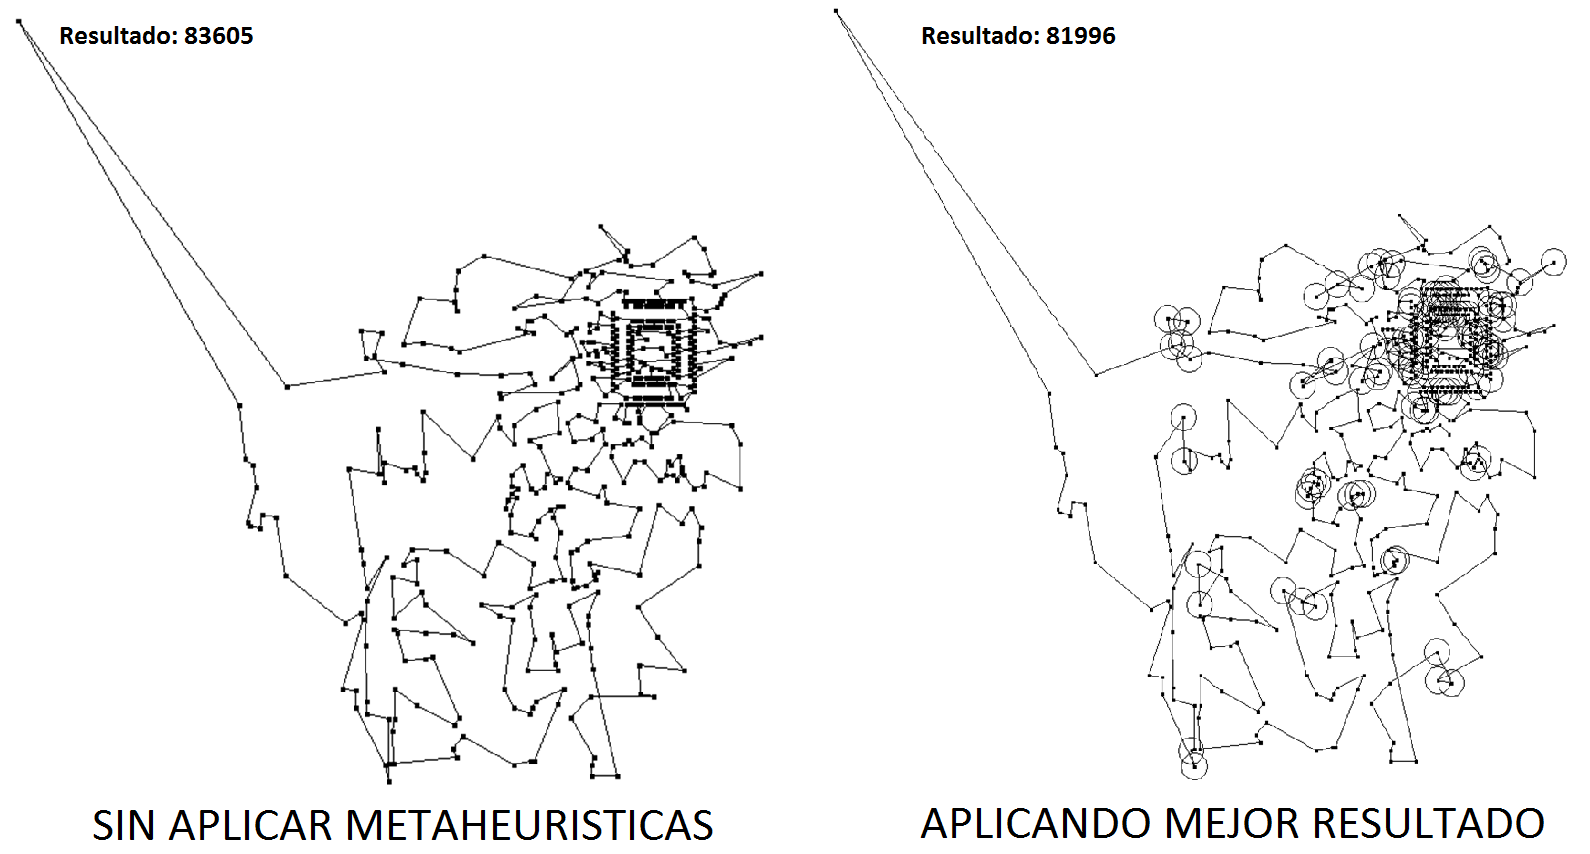
\includegraphics[width=1\textwidth]{PruebasResultados/Experimentos_Comparativas/d493.png}
        \caption{Comparativa d493.tsp.}
        \label{fig:d493_comparativa.png}
\end{figure}
 \begin{figure}[hbtp]
    \centering
        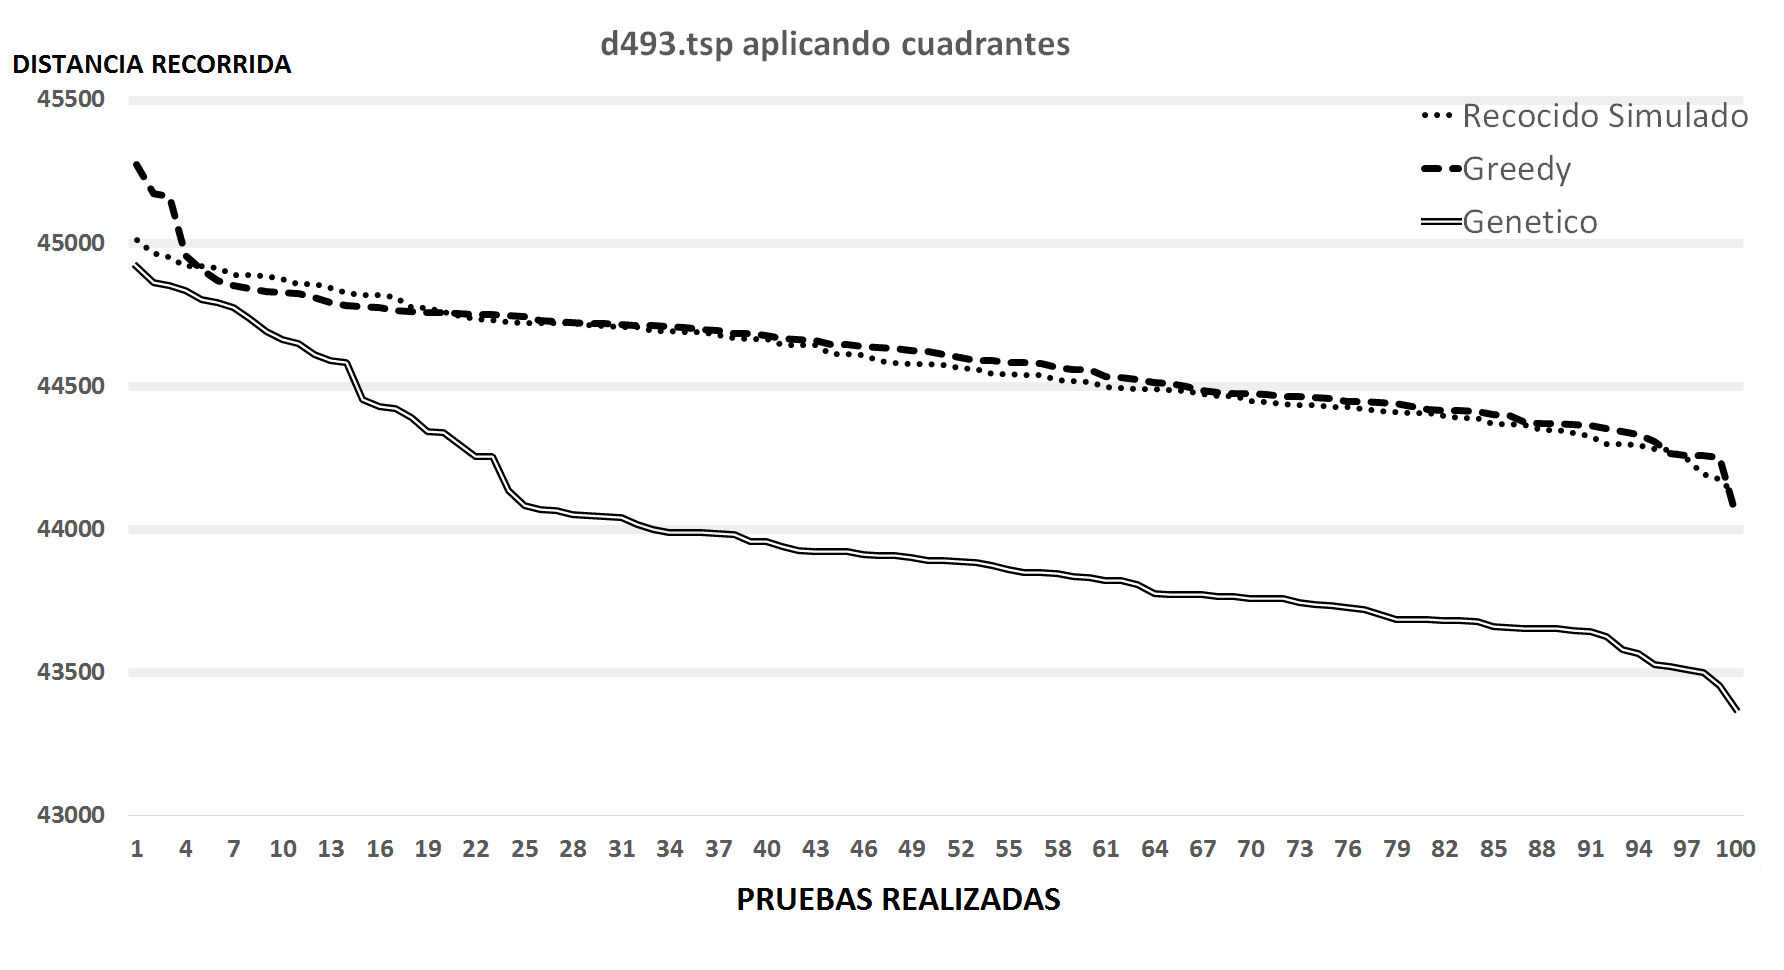
\includegraphics[width=1\textwidth]{PruebasResultados/Experimentos_Graficos_Con/d493.png}
        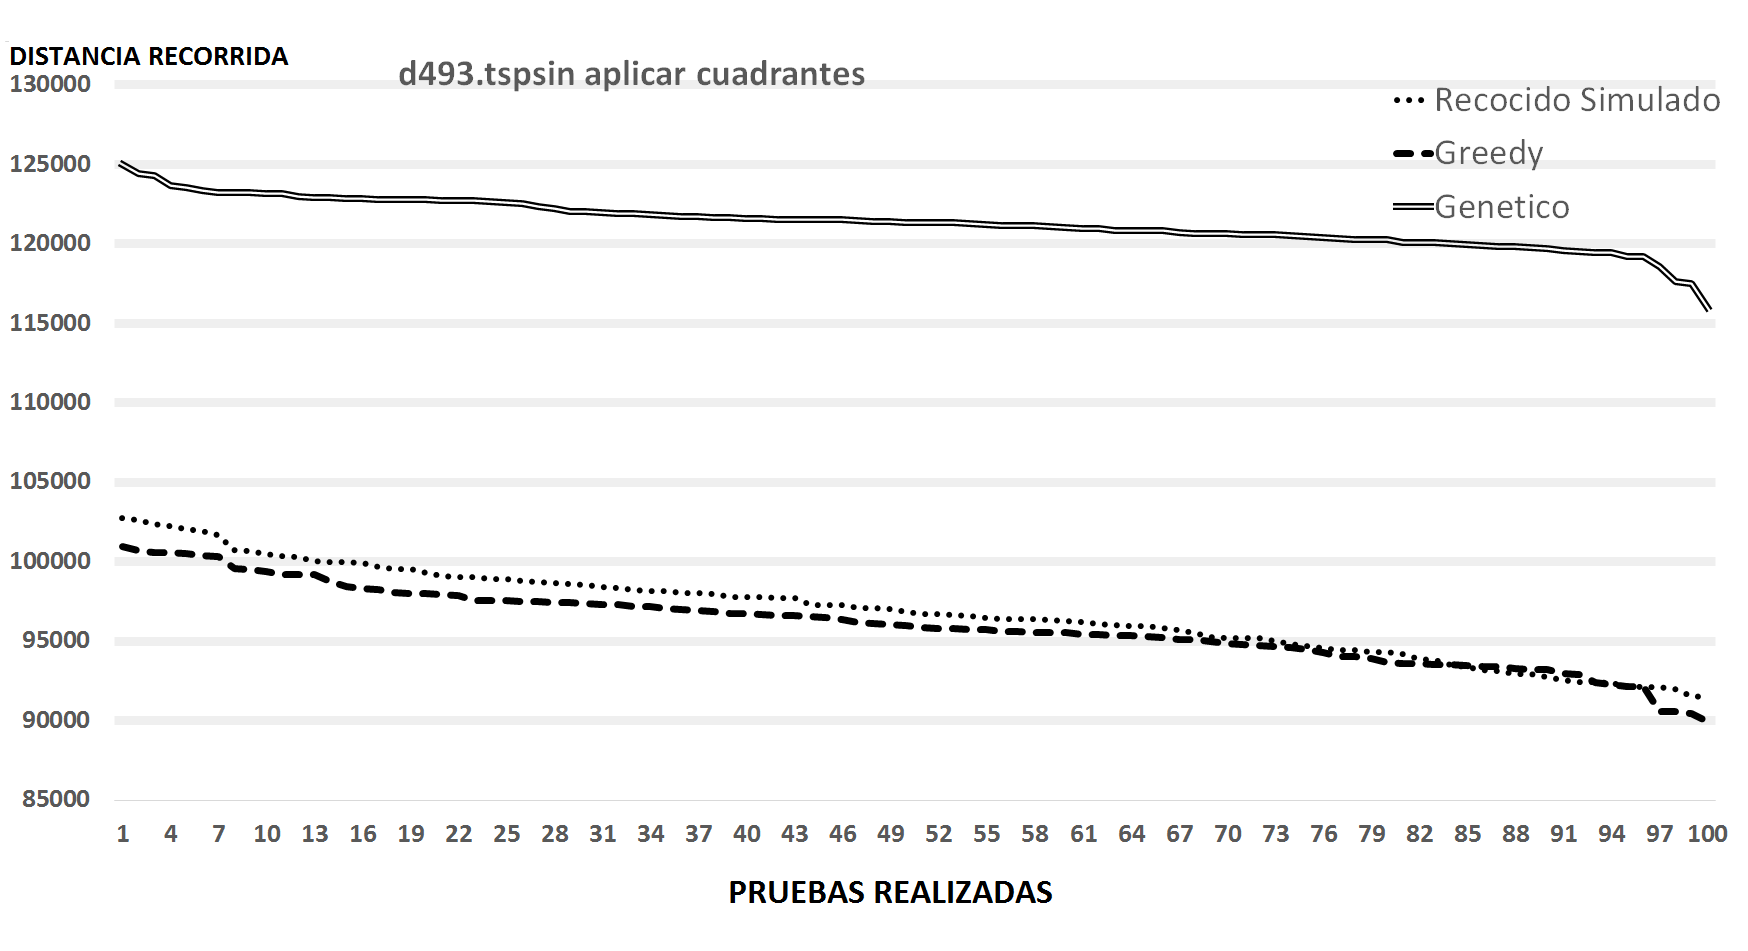
\includegraphics[width=1\textwidth]{PruebasResultados/Experimentos_Graficos_Sin/d493.png}
        \caption{Gráficos d493.tsp con cuadrantes y sin cuadrantes.}
        \label{fig:d493_grafica.png}
\end{figure}
\newpage

%EIL101.TSP
\subsubsection{eil101.TSP}
\begin{table}[hbtp]
 \centering
     \caption{Experimento con el problema eil101.tsp.}
\begin{tabular}{ | l   l | r | r | r |   }
	    \hline\multicolumn{5}{|c|}{ \rowcolor[gray]{0.8} eil101.tsp} \\ \hline
         \multicolumn{2}{|l|}{Resultado Original : 828}   & Promedio & Mejor & Peor \\ 
                \hline
                & Recocido  & 804.91 & 788 & 822  \\ 
 Con cuadrantes & Greedy    & 806.93 & 788 & 825  \\ 
                & Genético  & \cellcolor[gray]{0.9} 787.33 & \cellcolor[gray]{0.9} 781 & \cellcolor[gray]{0.9} 802  \\ 
                \hline
                & Recocido  & 1747.41 & \cellcolor[gray]{0.9} 1585 & 1917   \\ 
 Sin cuadrantes & Greedy    & 1744.97 & 1630 & 1855   \\ 
                & Genético  & \cellcolor[gray]{0.9} 1705.49 & 1602 & \cellcolor[gray]{0.9} 1740    \\ 
                \hline
    \end{tabular}
    \label{table:EXP_eil101.tsp}
\end{table}
 \begin{figure}[hbtp]
    \centering
        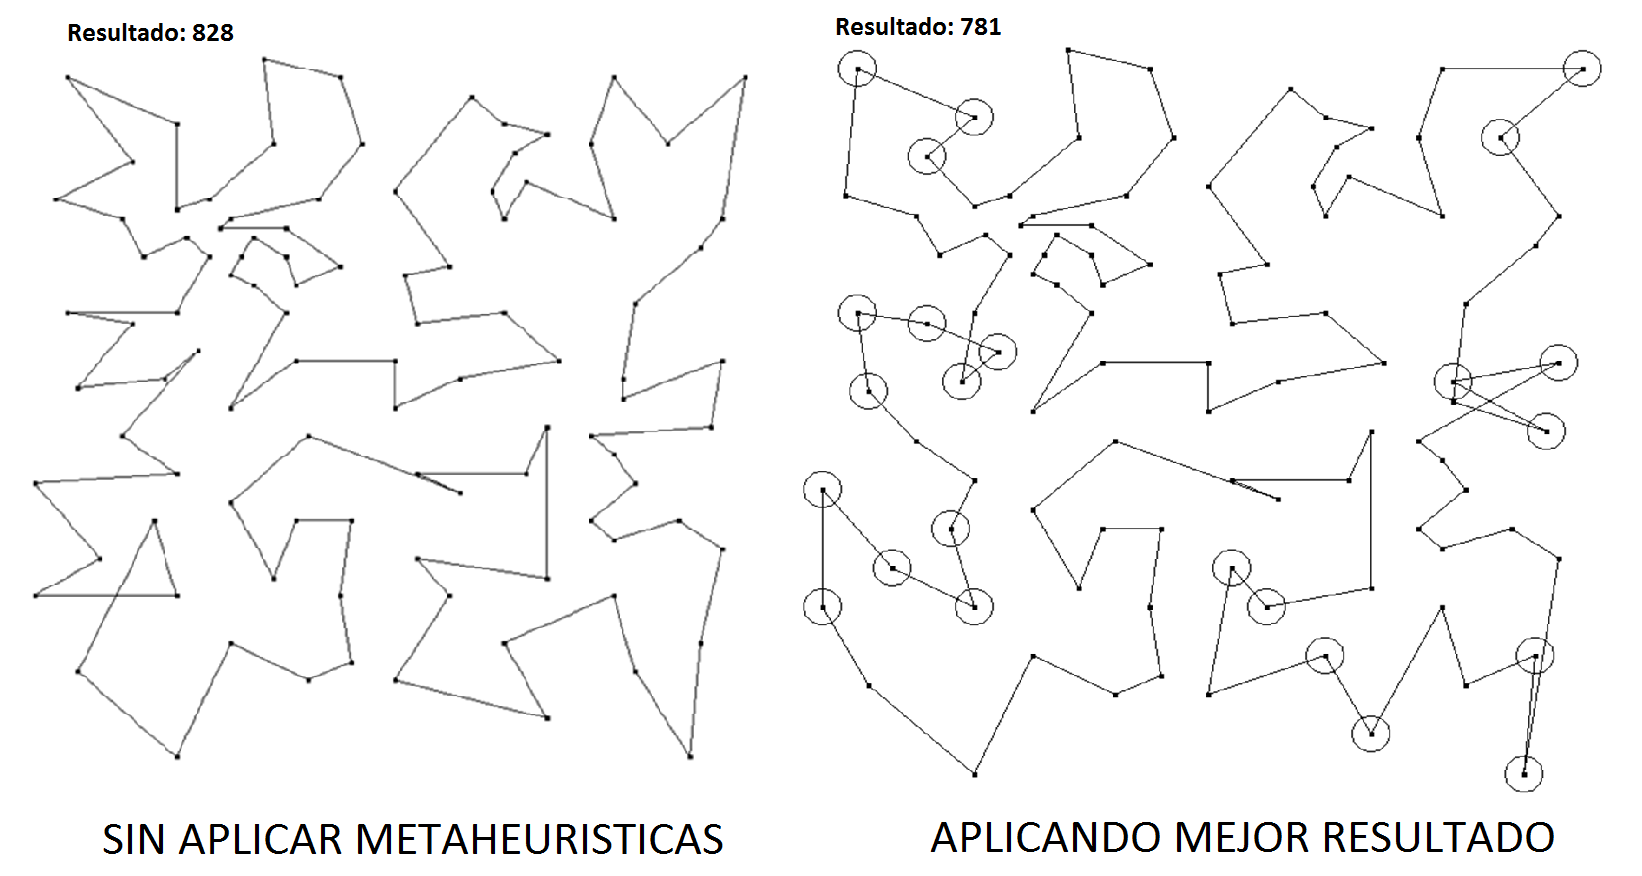
\includegraphics[width=1\textwidth]{PruebasResultados/Experimentos_Comparativas/eil101.png}
        \caption{Comparativa eil101.tsp.}
        \label{fig:eil101_comparativa.png}
\end{figure}
 \begin{figure}[hbtp]
    \centering
        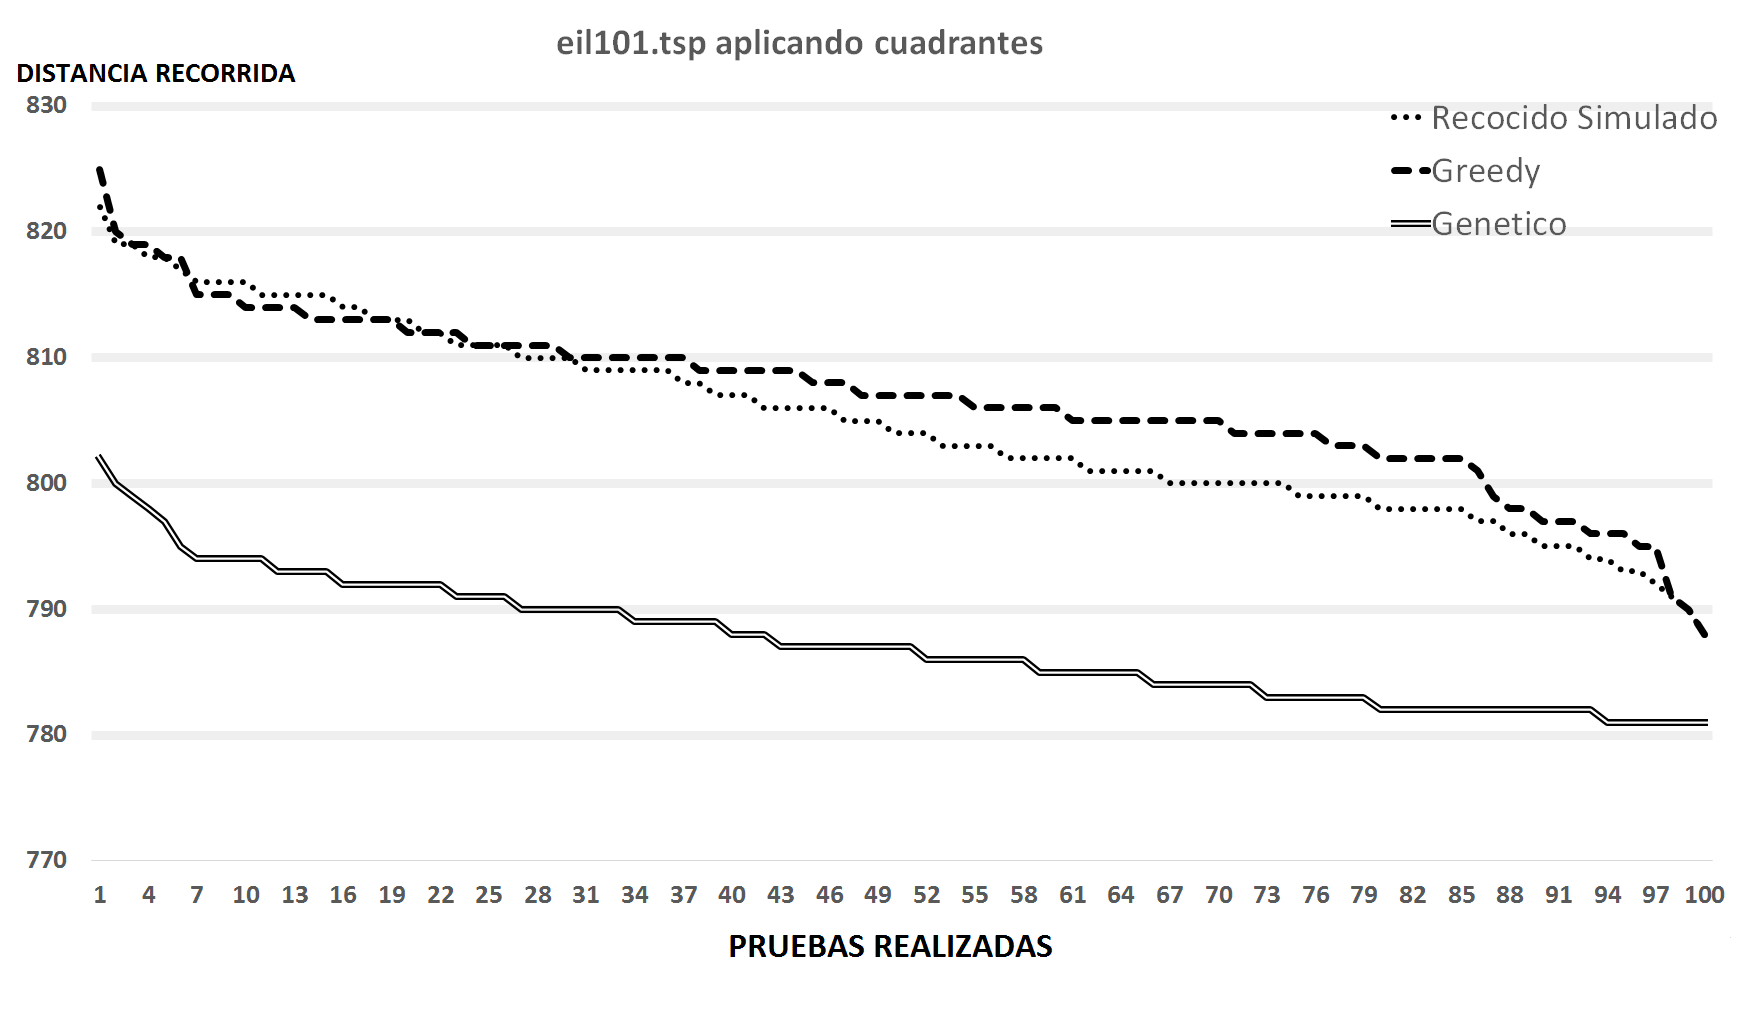
\includegraphics[width=1\textwidth]{PruebasResultados/Experimentos_Graficos_Con/eil101.png}
        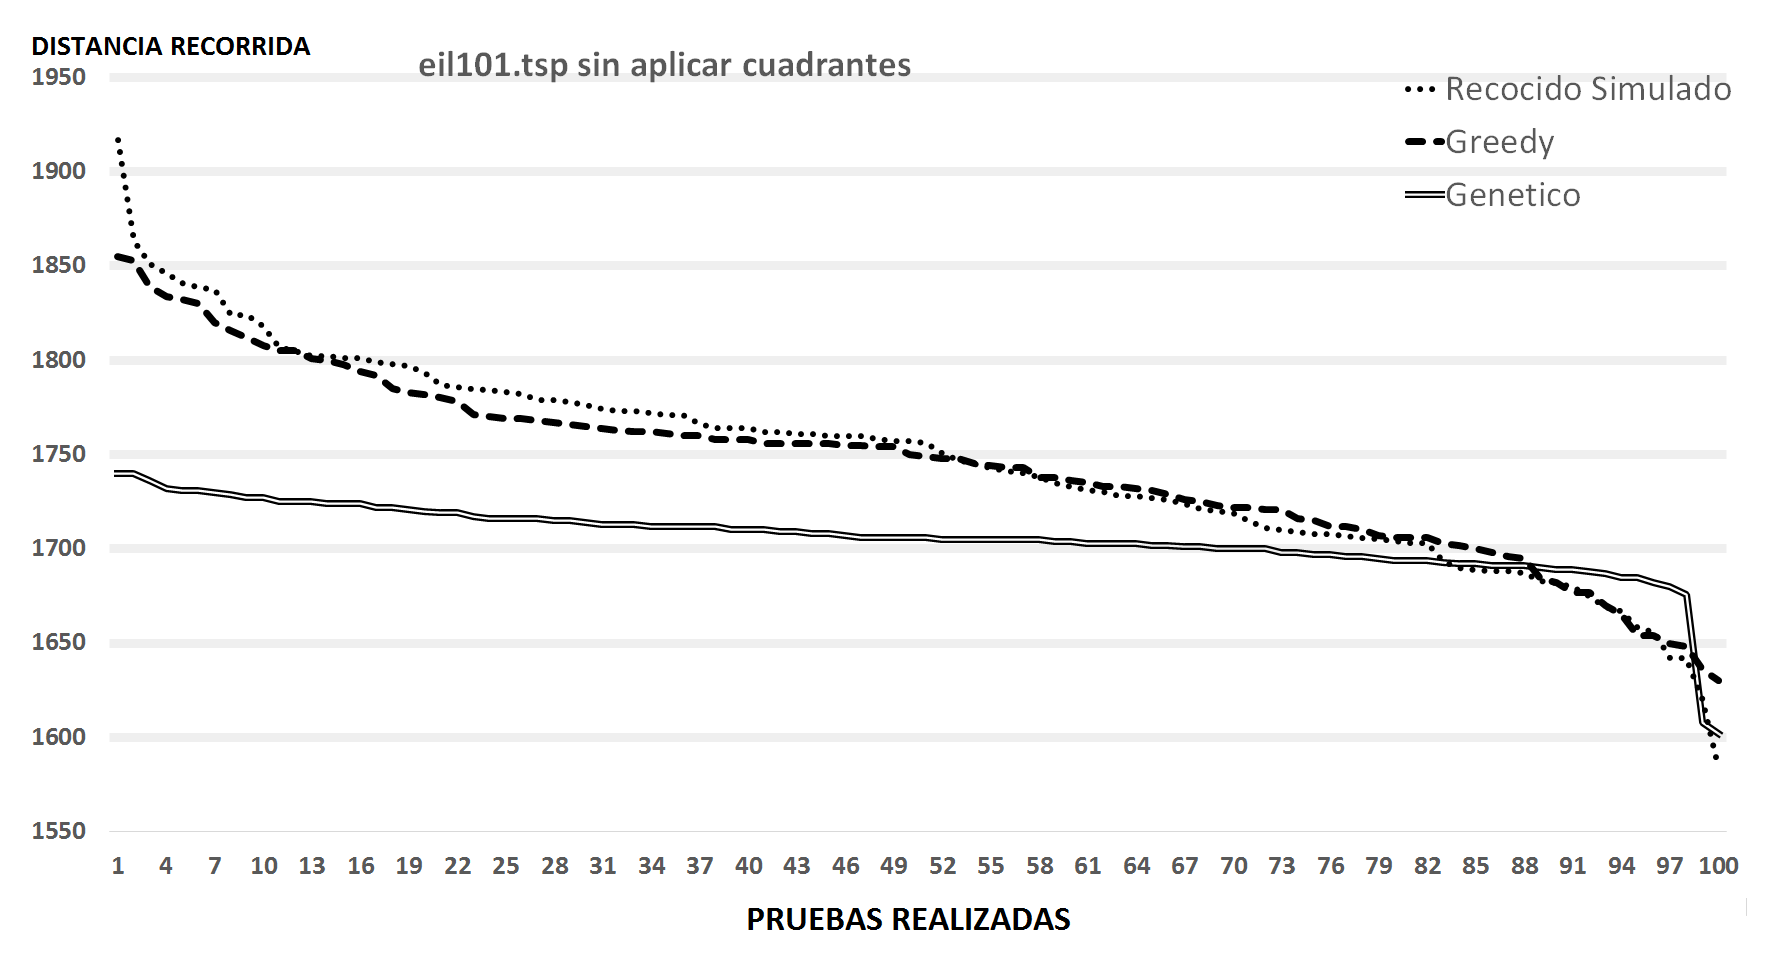
\includegraphics[width=1\textwidth]{PruebasResultados/Experimentos_Graficos_Sin/eil101.png}
        \caption{Gráficos eil101.tsp con cuadrantes y sin cuadrantes.}
        \label{fig:eil101_grafica.png}
\end{figure}
\newpage

%fl417.TSP
\subsubsection{fl417.TSP}
\begin{table}[hbtp]
 \centering 
    \caption{Experimento con el problema fl417.tsp.}
	\begin{tabular}{ | l   l | r | r | r |   }
       \hline\multicolumn{5}{|c|}{ \rowcolor[gray]{0.8} fl417.tsp} \\\hline
        \multicolumn{2}{|l|}{Resultado Original : 17419} & Promedio & Mejor & Peor \\ 
                \hline
                & Recocido  & 16835.95 & 16672 & 17070  \\ 
 Con cuadrantes & Greedy    & 16824.81 & 16610 & 17028  \\ 
                & Genético  & \cellcolor[gray]{0.9} 16599.01 & \cellcolor[gray]{0.9} 16450 & \cellcolor[gray]{0.9} 16709 \\ 
                \hline
                & Recocido  & 48845.13 & 46858 & 50870   \\ 
 Sin cuadrantes & Greedy    & \cellcolor[gray]{0.9} 48689.67 & \cellcolor[gray]{0.9} 46460 & \cellcolor[gray]{0.9} 50570 \\ 
                & Genético  & 52319.03 & 50896 & 53761    \\ 
                \hline
    \end{tabular}
    \label{table:EXP_fl417.tsp}
\end{table}
\begin{figure}[hbtp]
    \centering
        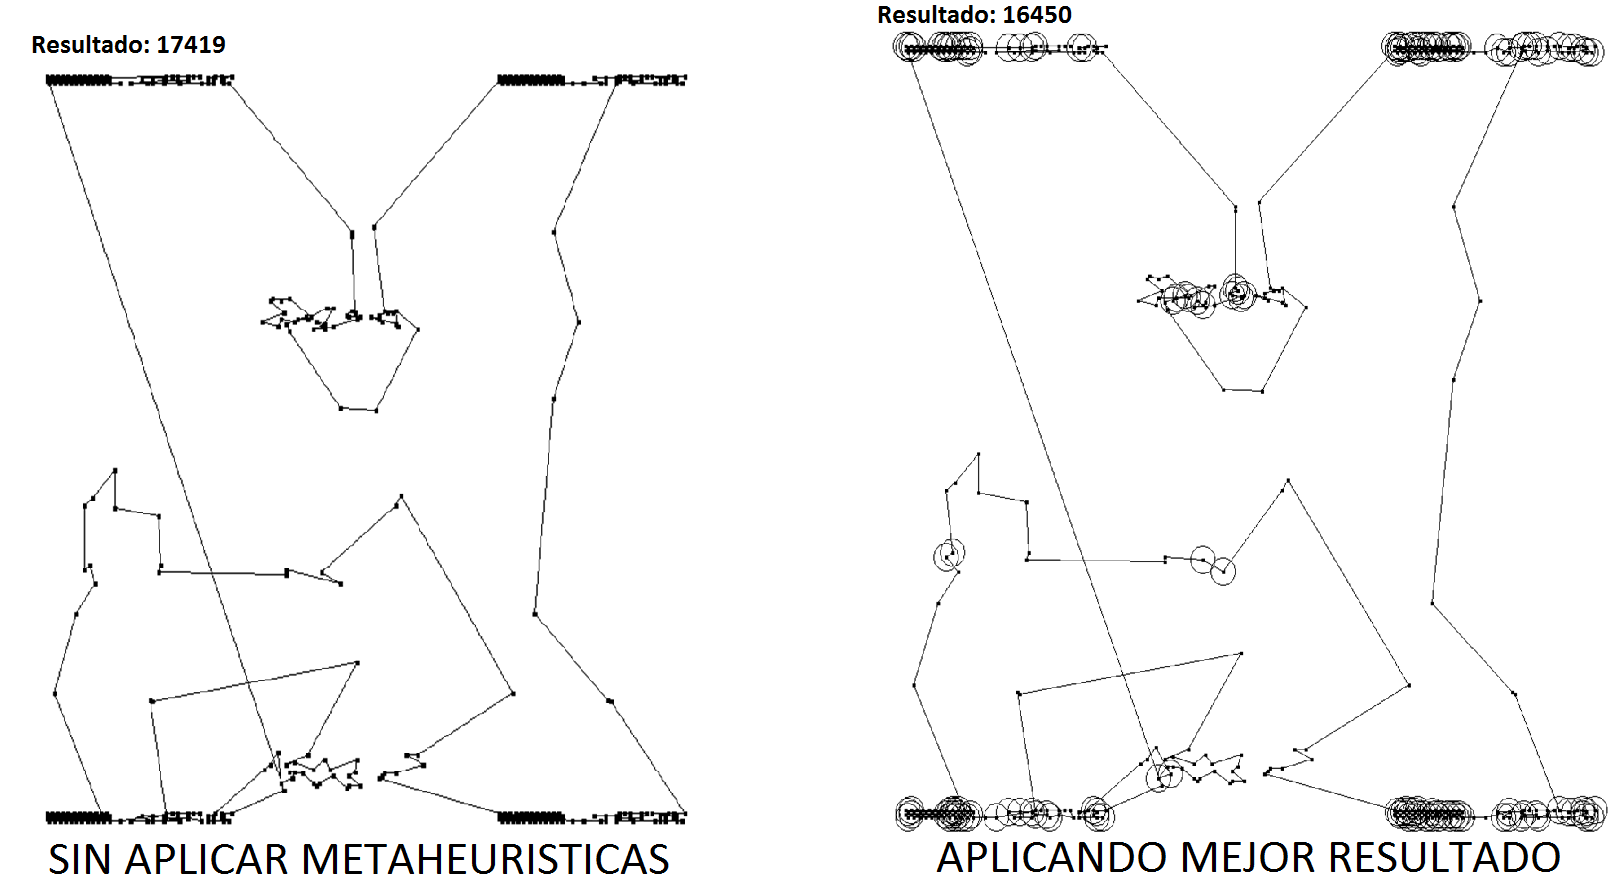
\includegraphics[width=1\textwidth]{PruebasResultados/Experimentos_Comparativas/fl417.png}
        \caption{Comparativa fl417.tsp.}
        \label{fig:fl417_comparativa.png}
\end{figure}
 \begin{figure}[hbtp]
    \centering
        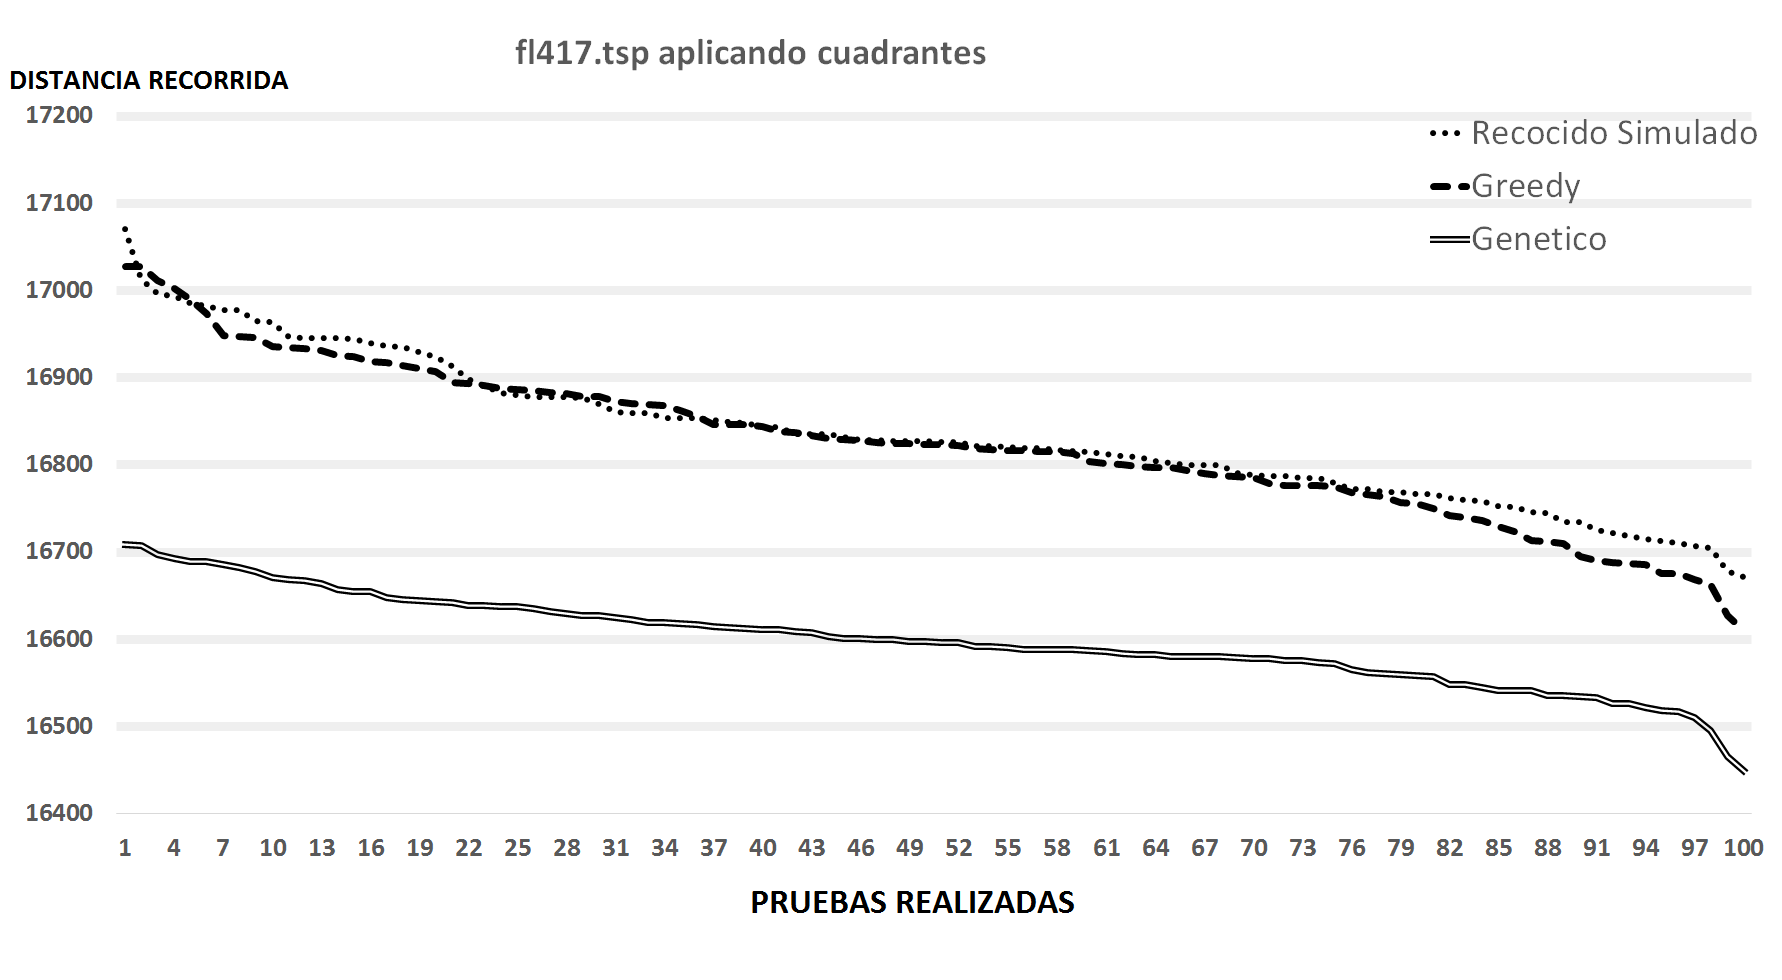
\includegraphics[width=1\textwidth]{PruebasResultados/Experimentos_Graficos_Con/fl417.png}
        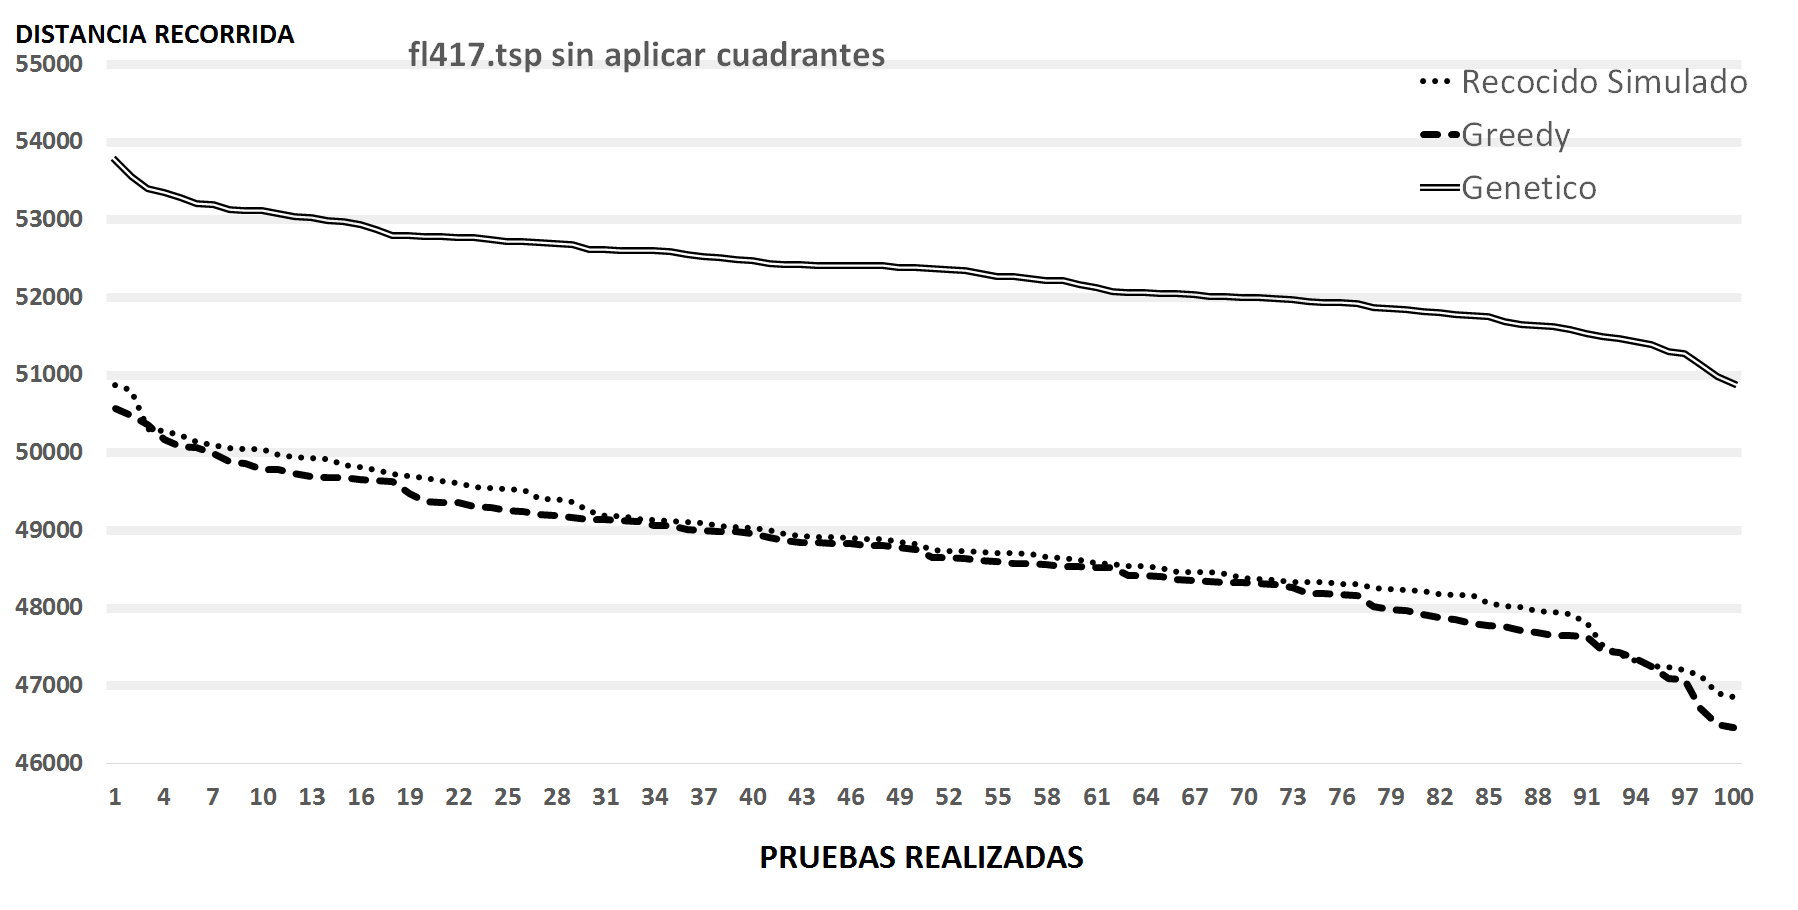
\includegraphics[width=1\textwidth]{PruebasResultados/Experimentos_Graficos_Sin/fl417.png}
        \caption{Gráficos fl417.tsp con cuadrantes y sin cuadrantes.}
        \label{fig:fl417_grafica.png}
\end{figure}
\newpage

%LIN318.TSP
\subsubsection{lin318.TSP}
\begin{table}[hbtp]
 \centering
    \caption{Experimento con el problema lin318.tsp.} 
	\begin{tabular}{ | l   l | r | r | r |   }
     \hline\multicolumn{5}{|c|}{ \rowcolor[gray]{0.8}lin318.tsp} \\\hline
     \multicolumn{2}{|l|}{Resultado Original : 55340} & Promedio & Mejor & Peor \\ \hline
                & Recocido  & 54438.22 & 53752 & 55085  \\ 
 Con cuadrantes & Greedy    & 54367.97 & 53773 & 55073  \\ 
                & Genético  & \cellcolor[gray]{0.9} 53997.96 & \cellcolor[gray]{0.9} 53479 & \cellcolor[gray]{0.9} 54344  \\ 
                \hline
                & Recocido  & 110739.67 & \cellcolor[gray]{0.9} 102042 & 118920   \\ 
 Sin cuadrantes & Greedy    & \cellcolor[gray]{0.9} 110691.43 & 104454 & \cellcolor[gray]{0.9} 117441   \\ 
                & Genético  & 120441.11 & 114461 & 125074    \\ 
                \hline
    \end{tabular}
    \label{table:EXP_lin318.tsp}
\end{table}
 \begin{figure}[hbtp]
    \centering
        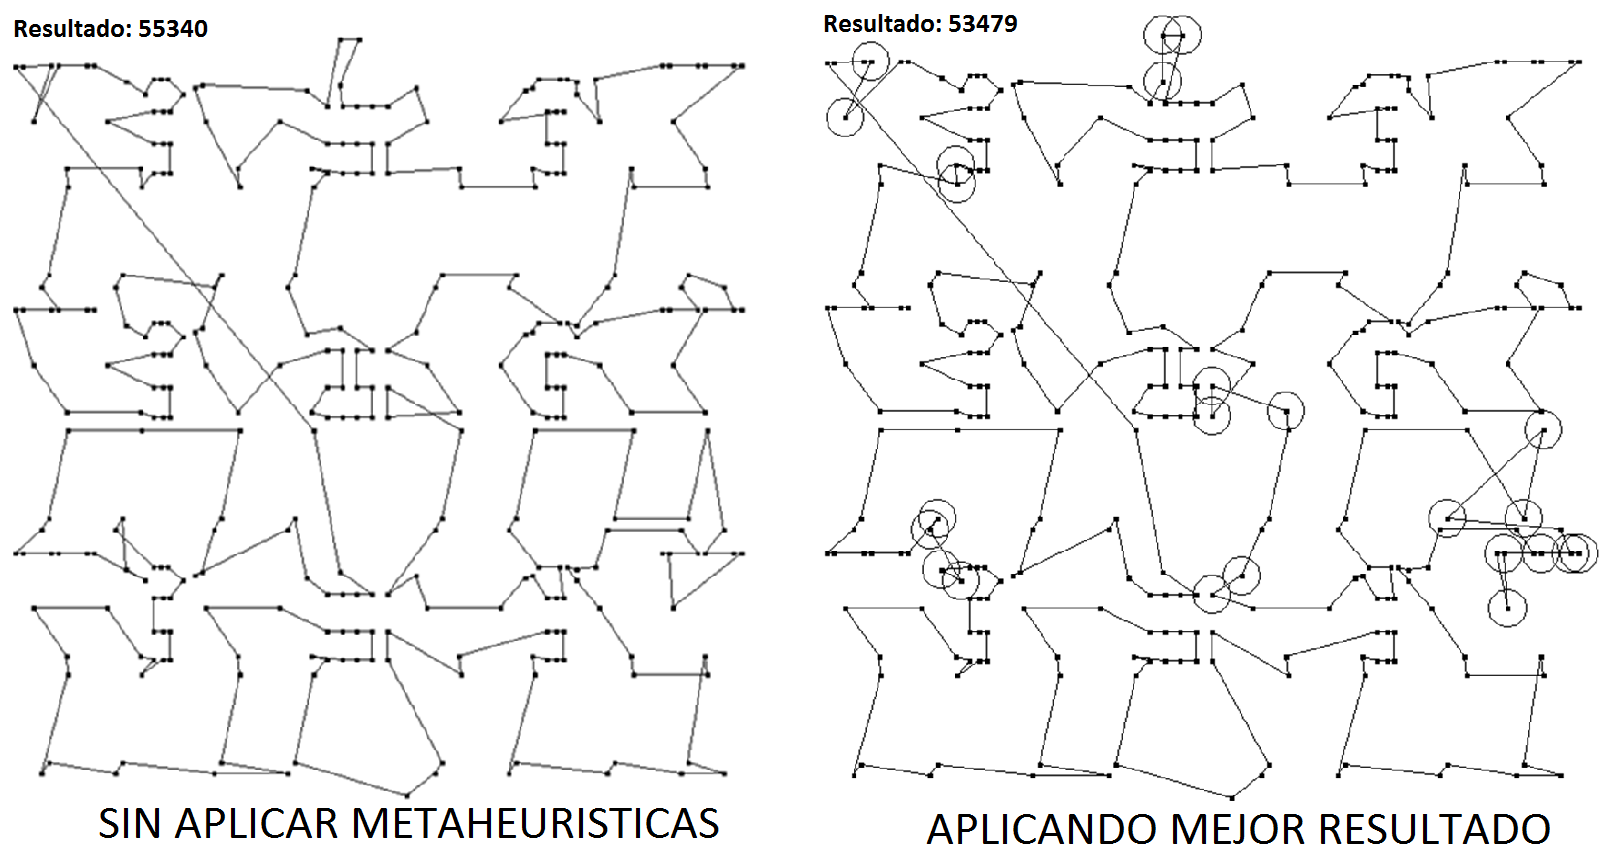
\includegraphics[width=1\textwidth]{PruebasResultados/Experimentos_Comparativas/lin318.png}
        \caption{Comparativa lin318.tsp.}
        \label{fig:lin318_comparativa.png}
\end{figure}
 \begin{figure}[hbtp]
    \centering
        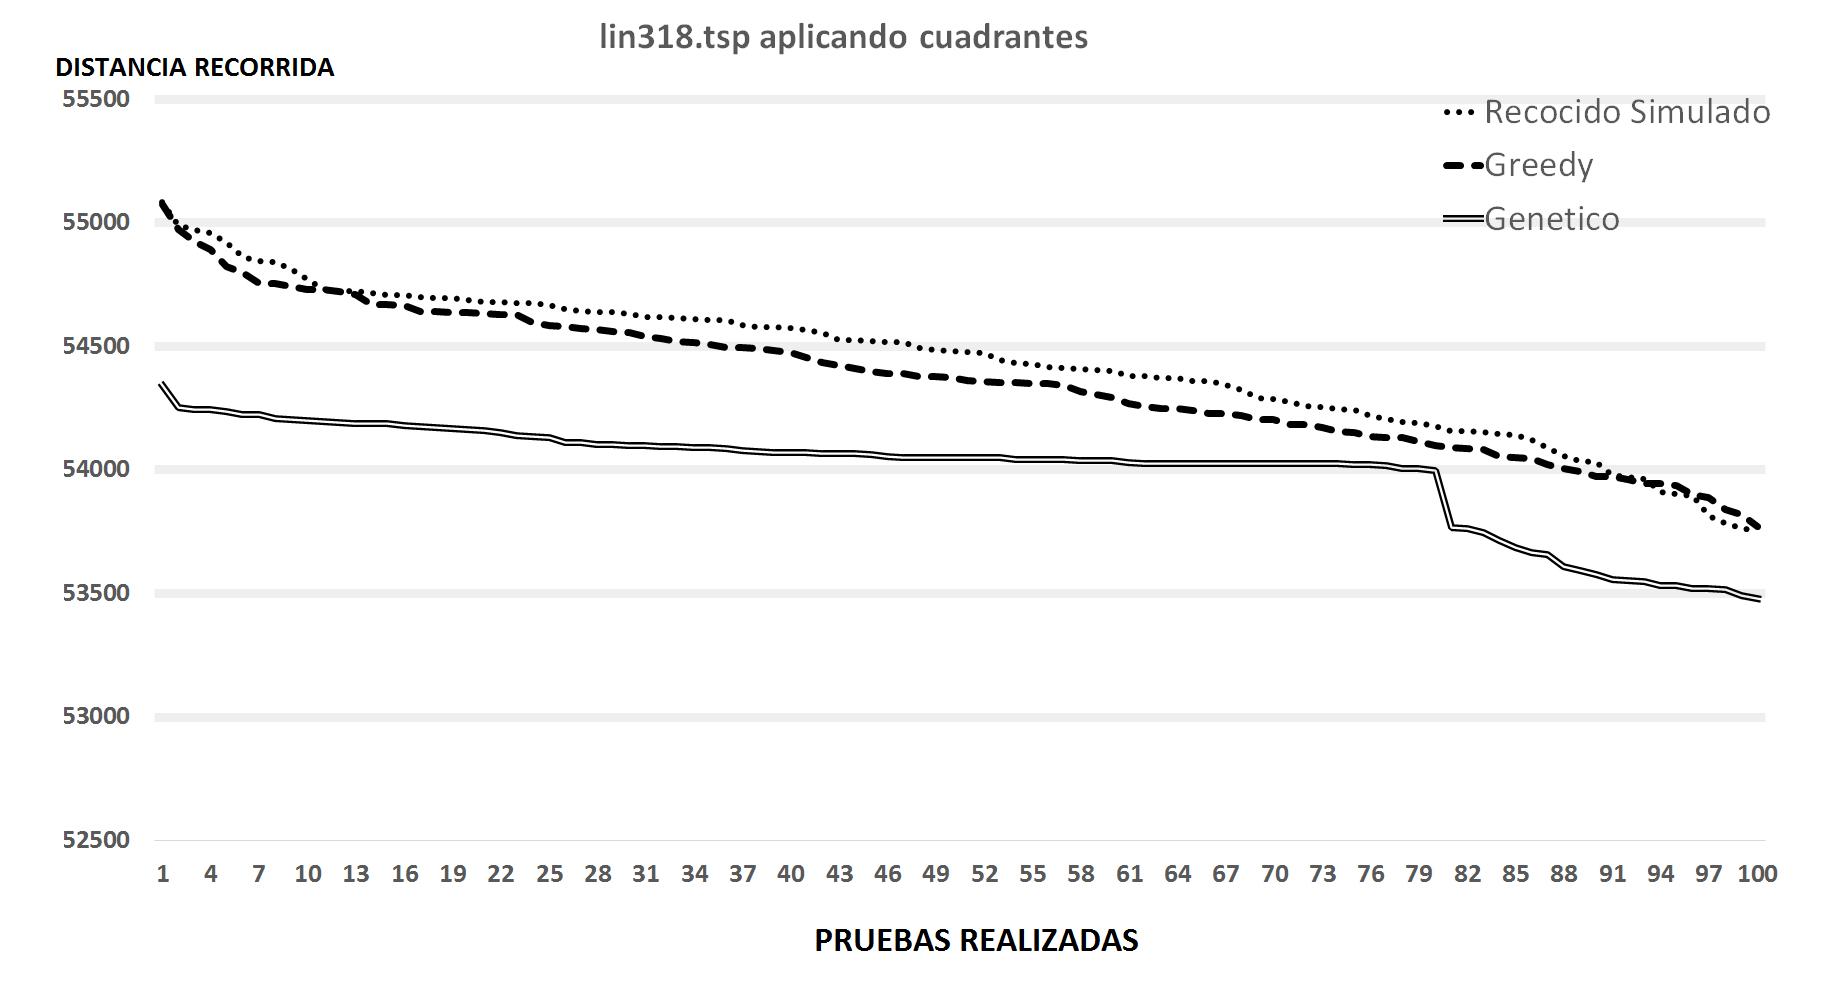
\includegraphics[width=1\textwidth]{PruebasResultados/Experimentos_Graficos_Con/lin318.png}
        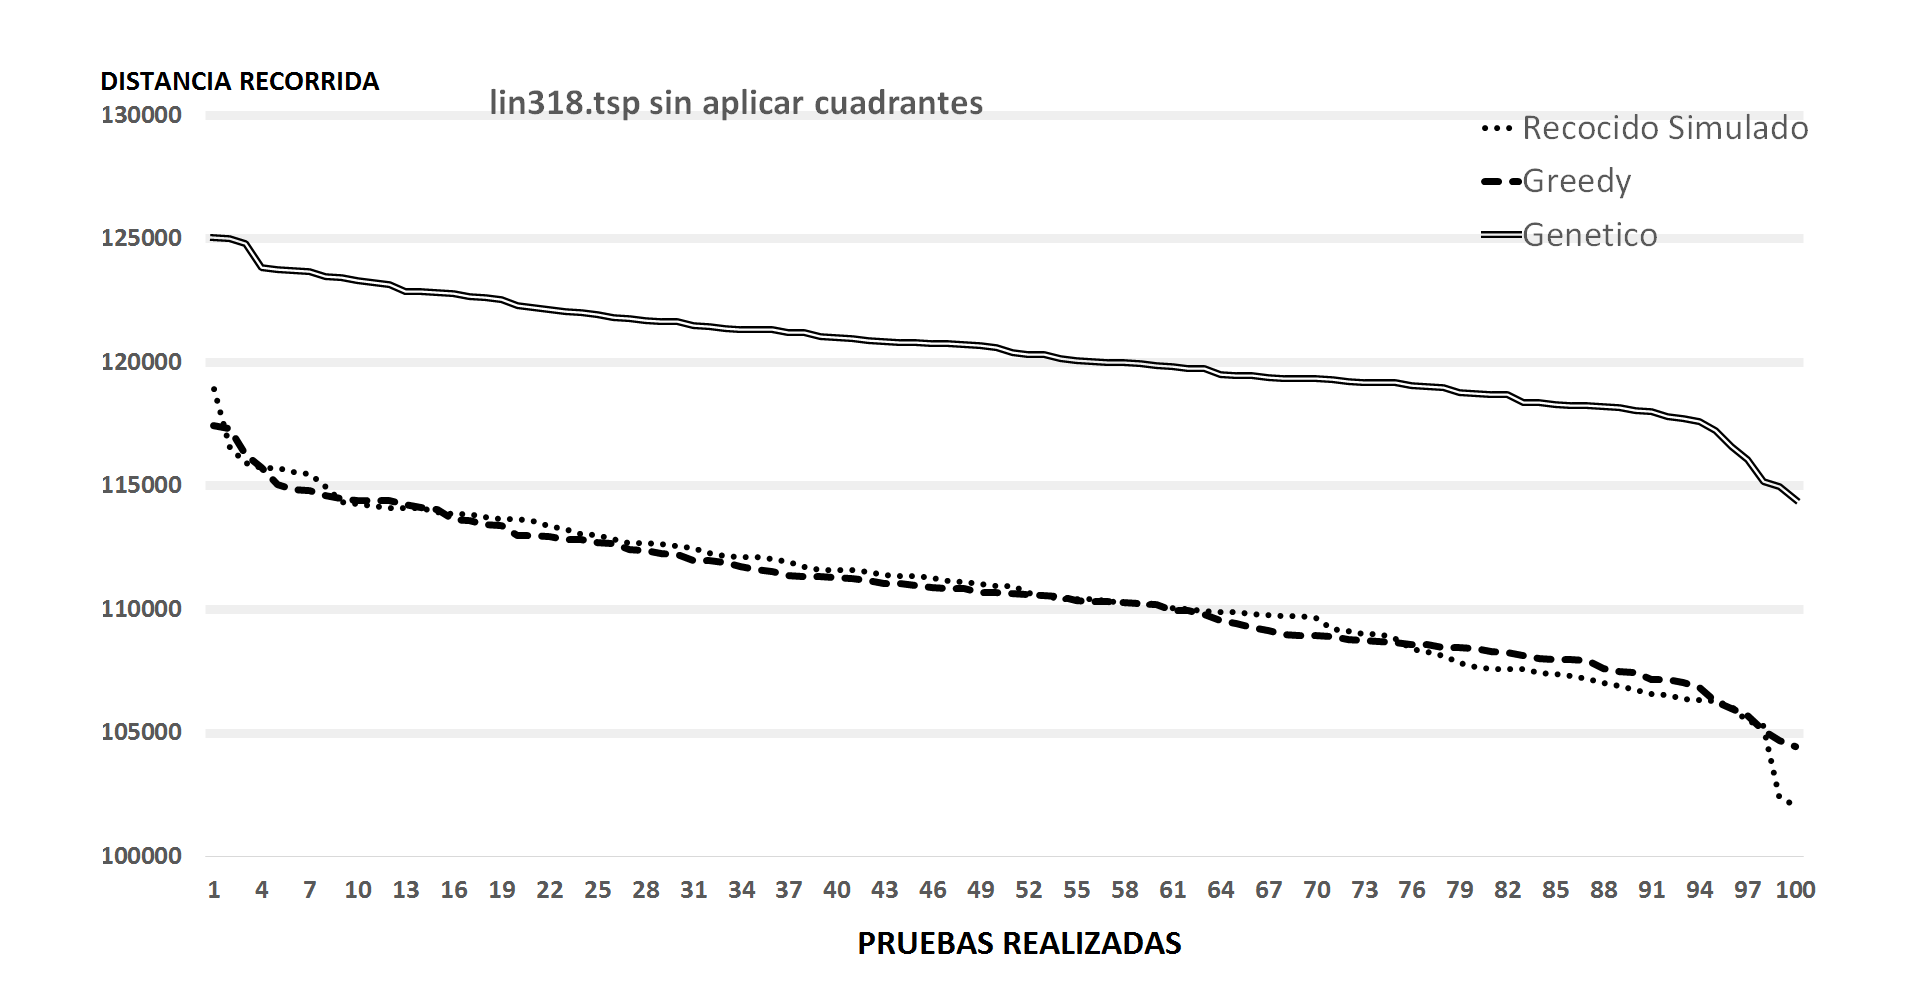
\includegraphics[width=1\textwidth]{PruebasResultados/Experimentos_Graficos_Sin/lin318.png}
        \caption{Gráficos lin318.tsp con cuadrantes y sin cuadrantes.}
        \label{fig:lin318_grafica.png}
\end{figure}
\newpage

%P654.TSP
\subsubsection{p654.TSP}
\begin{table}[hbtp]
 \centering 
    \caption{Experimento con el problema p654.tsp.}
	\begin{tabular}{ | l   l | r | r | r |   }
        \hline\multicolumn{5}{|c|}{ \rowcolor[gray]{0.8}p654.tsp} \\\hline
         \multicolumn{2}{|l|}{Resultado Original : 47464} & Promedio & Mejor & Peor \\ \hline
                & Recocido  & 46190.13 & 45753 & 46767  \\ 
 Con cuadrantes & Greedy    & 46146.53 & \cellcolor[gray]{0.9} 45588 & 46541  \\ 
                & Genético  &\cellcolor[gray]{0.9}  45916.31 & 45645 & \cellcolor[gray]{0.9} 46292  \\ 
                \hline
                & Recocido  & 121597.61 & \cellcolor[gray]{0.9} 118683 & 127226   \\ 
 Sin cuadrantes & Greedy    & \cellcolor[gray]{0.9} 121537.77 & 118676 & \cellcolor[gray]{0.9} 126211   \\ 
                & Genético  & 132643.30 & 131454 & 135144    \\ 
                \hline
    \end{tabular}
    \label{table:EXP_p654.tsp}
\end{table}
\begin{figure}[hbtp]
    \centering
        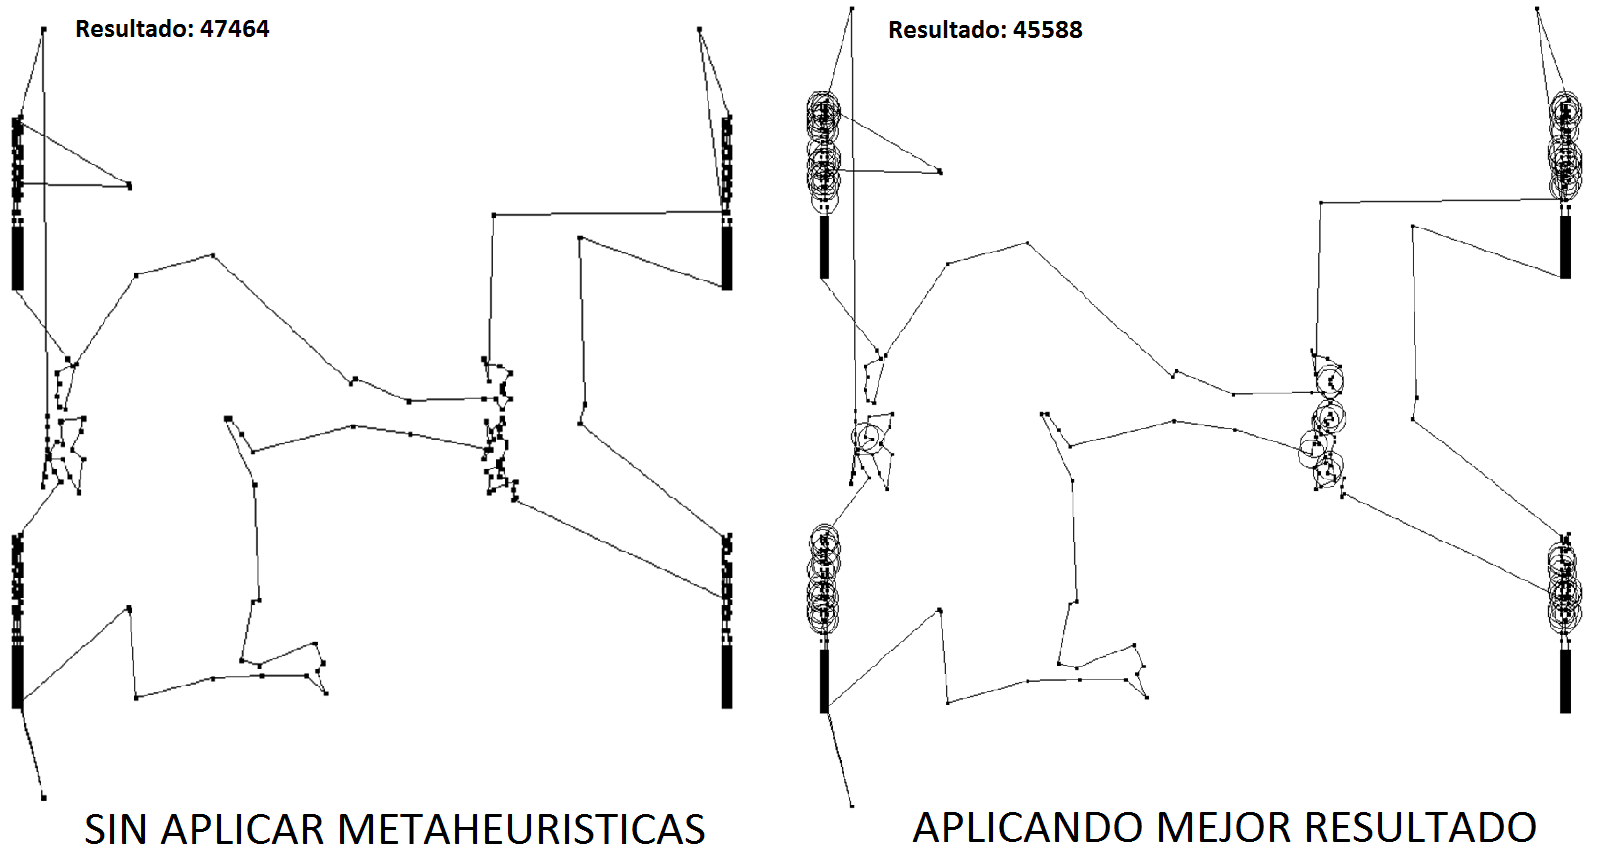
\includegraphics[width=1\textwidth]{PruebasResultados/Experimentos_Comparativas/p654.png}
        \caption{Comparativa p654.tsp.}
        \label{fig:p654_comparativa.png}
\end{figure}
 \begin{figure}[hbtp]
    \centering
        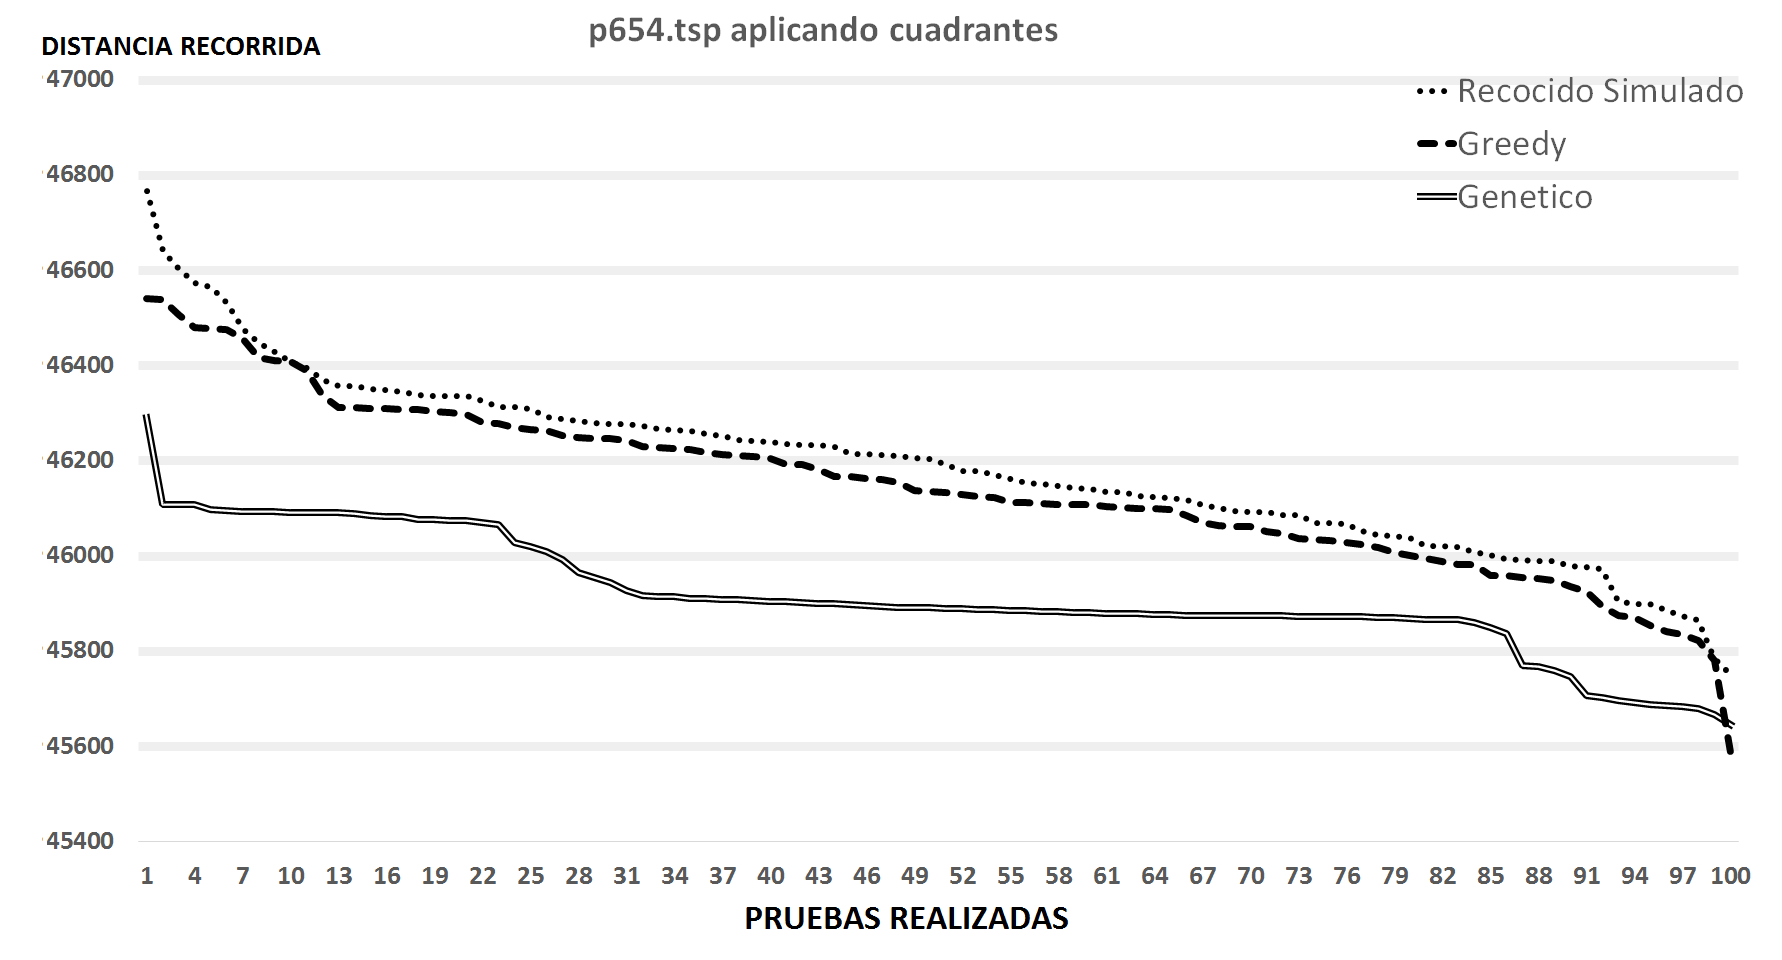
\includegraphics[width=1\textwidth]{PruebasResultados/Experimentos_Graficos_Con/p654.png}
        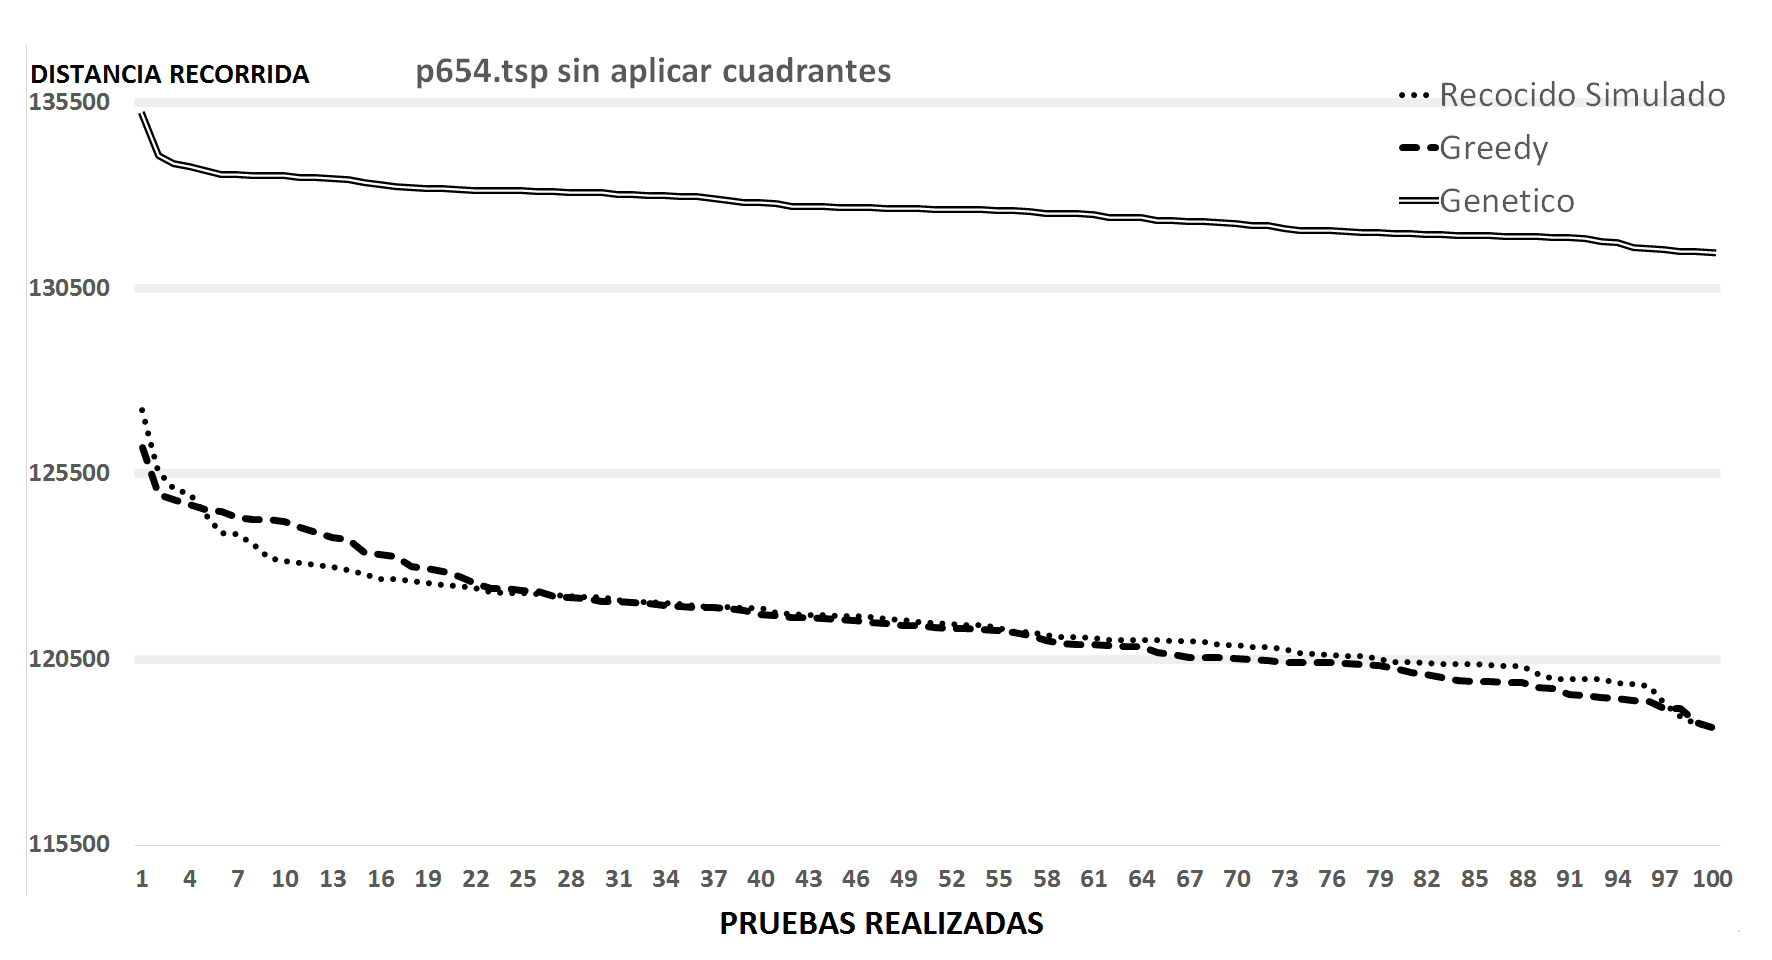
\includegraphics[width=1\textwidth]{PruebasResultados/Experimentos_Graficos_Sin/p654.png}
        \caption{Gráficos p654.tsp con cuadrantes y sin cuadrantes.}
        \label{fig:p654_grafica.png}
\end{figure}
\newpage

%pcb3038.TSP
\subsubsection{pcb3038.TSP}
\begin{table}[hbtp]
 \centering 
    \caption{Experimento con el problema pcb3038.tsp.} 
	\begin{tabular}{ | l   l | r | r | r |   }
        \hline\multicolumn{5}{|c|}{ \rowcolor[gray]{0.8}pcb3038.tsp} \\\hline
        \multicolumn{2}{|l|}{Resultado Original :179474}  & Promedio & Mejor & Peor \\ \hline
                & Recocido  & 176904.37 & 176488 & 177468  \\ 
 Con cuadrantes & Greedy    & \cellcolor[gray]{0.9} 176903.86 & \cellcolor[gray]{0.9} 176282 & \cellcolor[gray]{0.9} 177403  \\ 
                & Genético  & 176989.64 & 176391 & 177957  \\ 
                \hline
                & Recocido  & \cellcolor[gray]{0.9} 389970.63 & 384530 & \cellcolor[gray]{0.9} 396772   \\ 
 Sin cuadrantes & Greedy    & 390708.99 & \cellcolor[gray]{0.9} 382955 & 398492   \\ 
                & Genético  & 425459.53 & 422981 & 427722   \\ 
                \hline
    \end{tabular}
    \label{table:EXP_pcb3038.tsp}
\end{table}
\begin{figure}[hbtp]
    \centering
        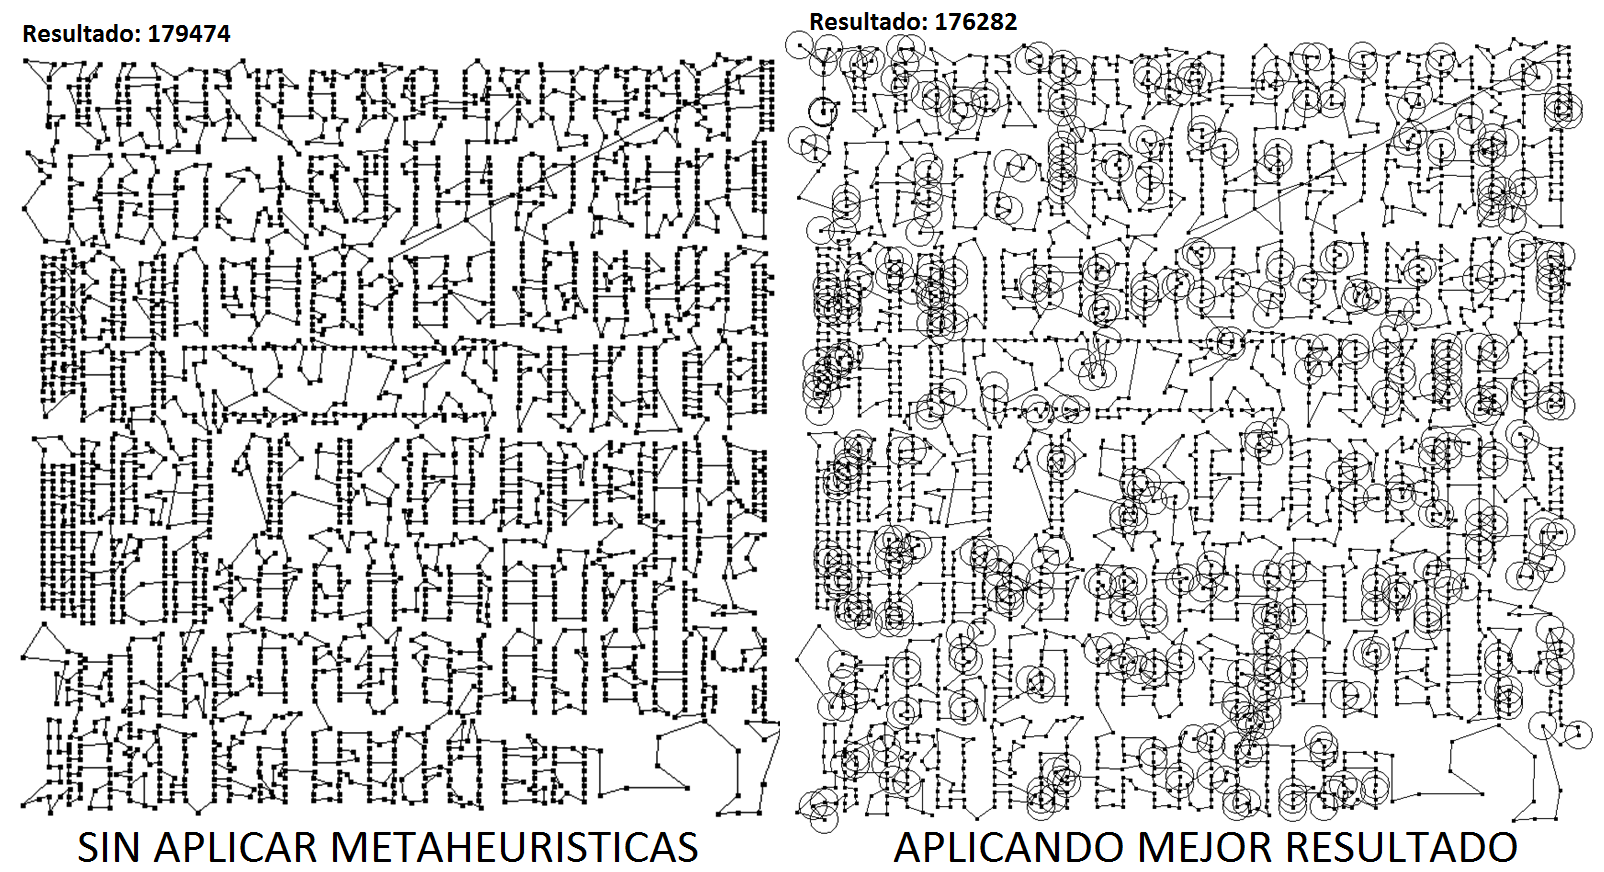
\includegraphics[width=1\textwidth]{PruebasResultados/Experimentos_Comparativas/pcb3038.png}
        \caption{Comparativa pcb3038.tsp.}
        \label{fig:pcb3038_comparativa.png}
\end{figure}
 \begin{figure}[hbtp]
    \centering
        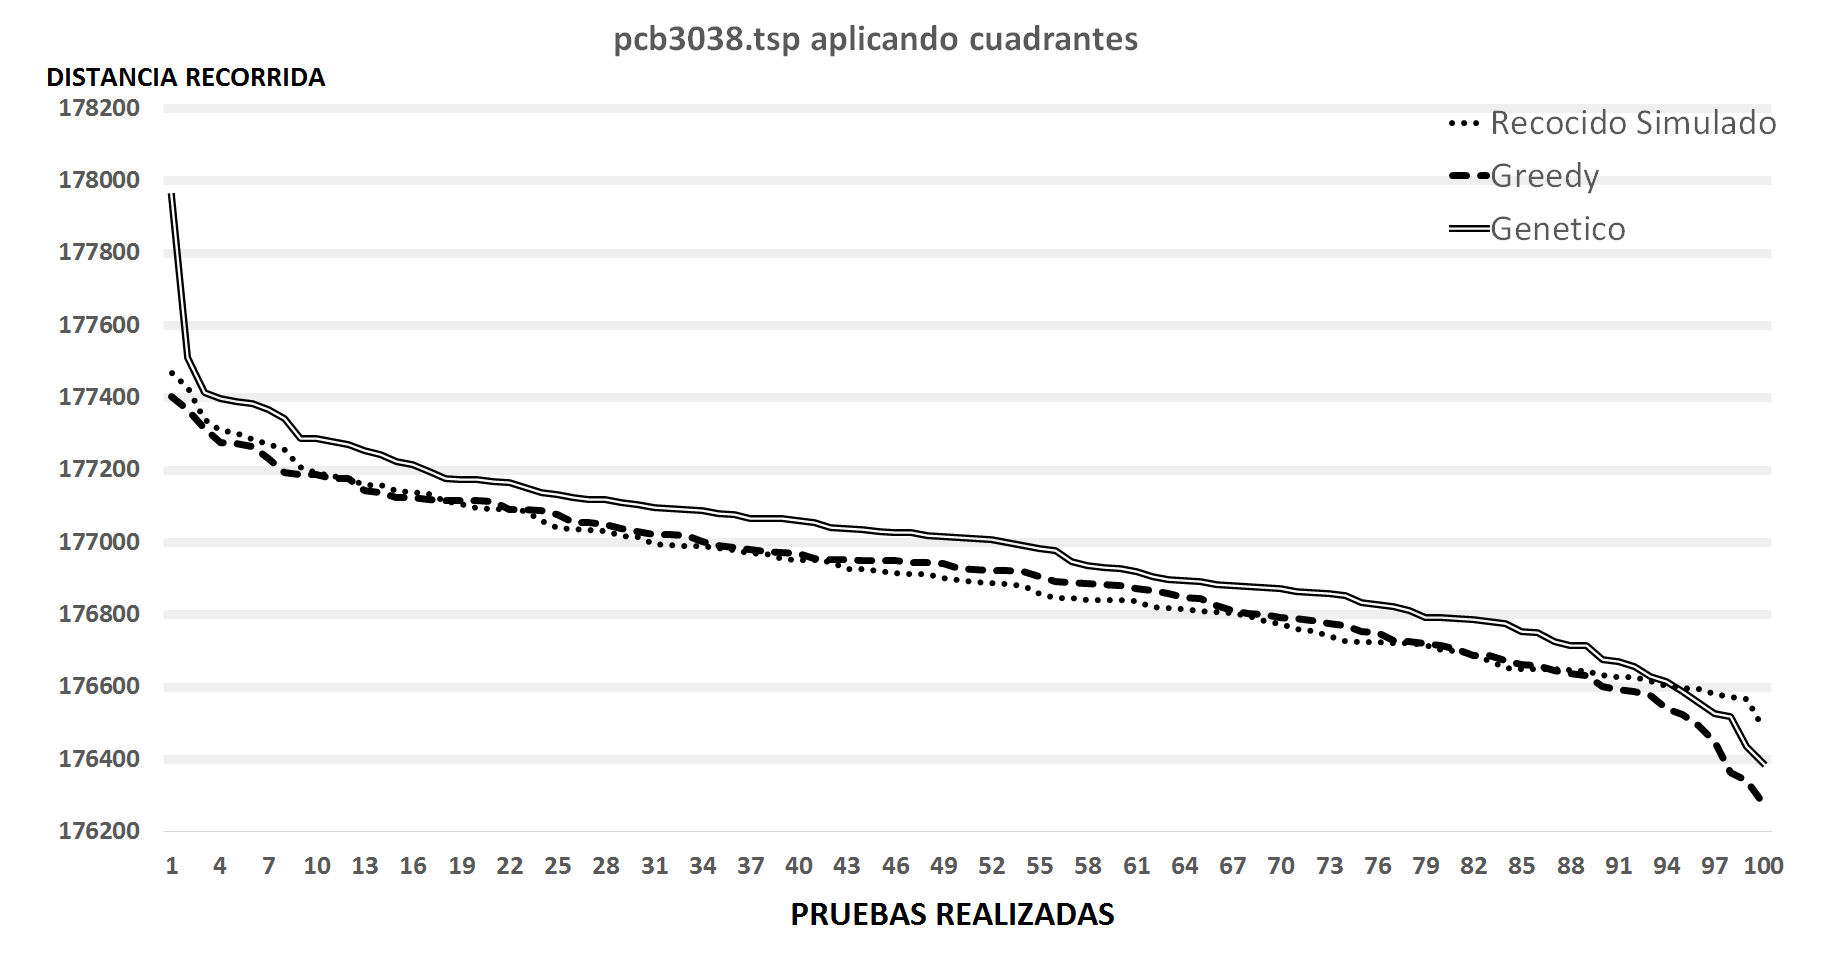
\includegraphics[width=1\textwidth]{PruebasResultados/Experimentos_Graficos_Con/pcb3038.png}
        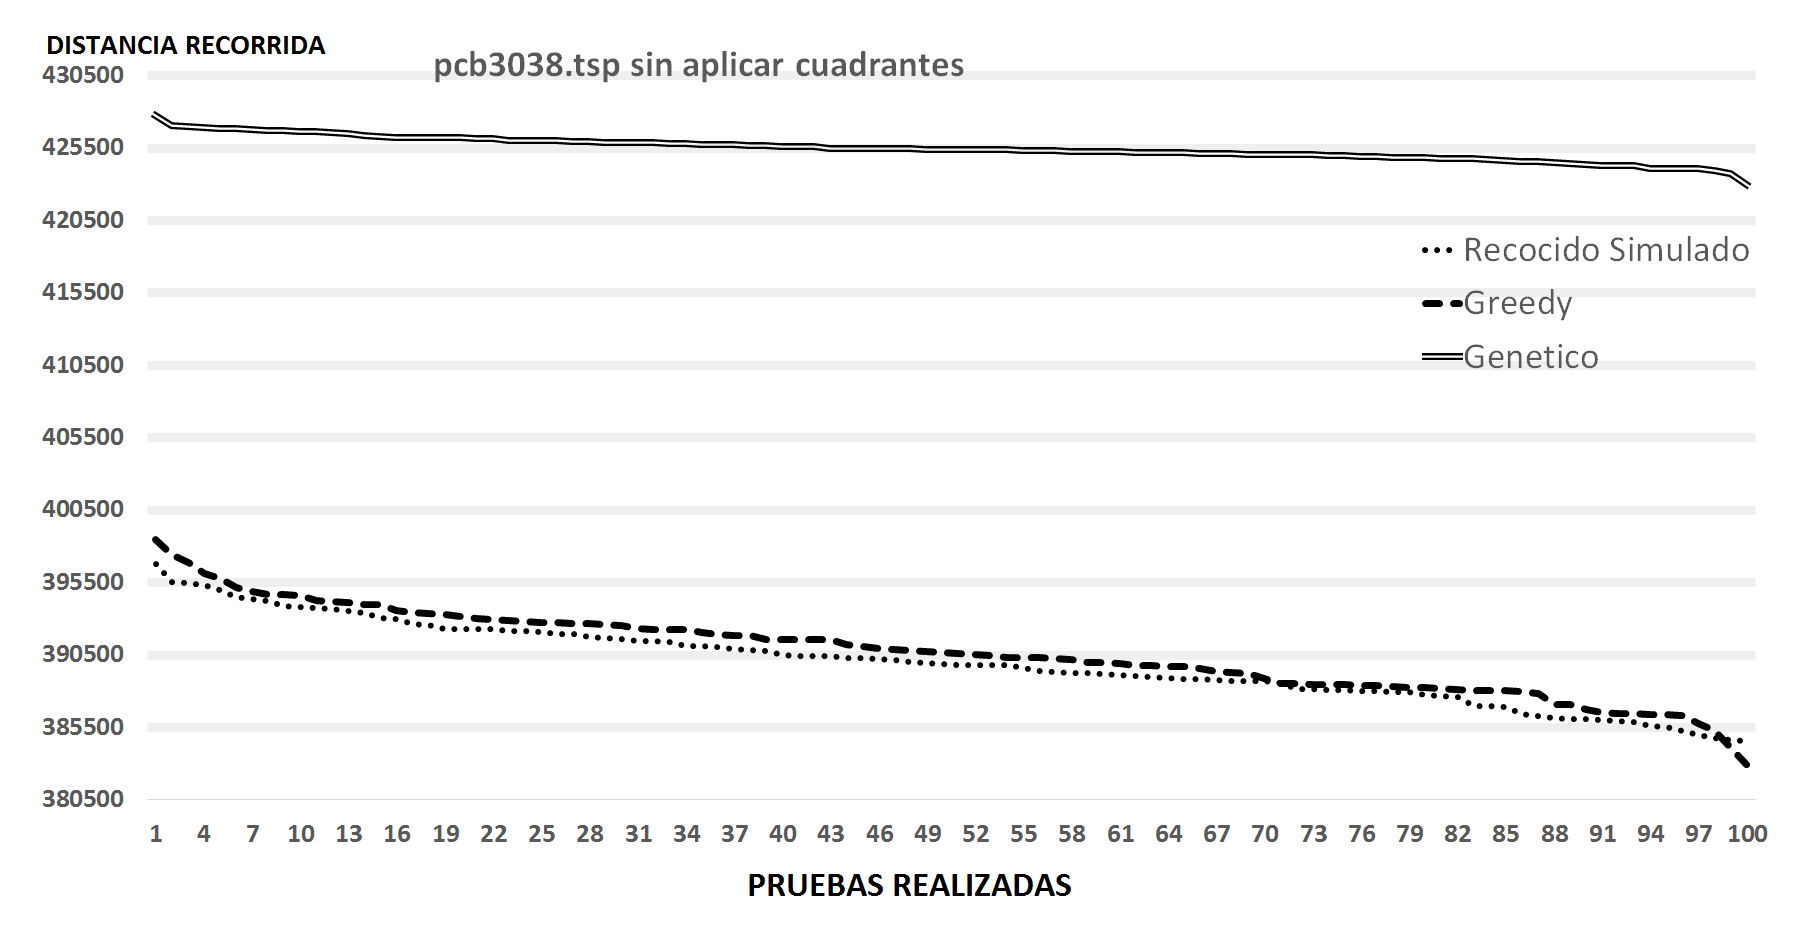
\includegraphics[width=1\textwidth]{PruebasResultados/Experimentos_Graficos_Sin/pcb3038.png}
        \caption{Gráficos pcb3038.tsp con cuadrantes y sin cuadrantes.}
        \label{fig:pcb3038_grafica.png}
\end{figure}
\newpage

%rd400.TSP
\subsubsection{rd400.TSP}
\begin{table}[hbtp]
 \centering 
    \caption{Experimento con el problema rd400.tsp.} 
	\begin{tabular}{ | l   l | r | r | r |   }
        \hline\multicolumn{5}{|c|}{ \rowcolor[gray]{0.8}rd400.tsp } \\\hline
         \multicolumn{2}{|l|}{Resultado Original : 19094} & Promedio & Mejor & Peor \\ \hline
                & Recocido  & 18773.66 & 18562 & 18922  \\ 
 Con cuadrantes & Greedy    & 18766.69 & 18559 & 18919  \\ 
                & Genético  & \cellcolor[gray]{0.9} 18633.28 & \cellcolor[gray]{0.9} 18510 & \cellcolor[gray]{0.9} 18790 \\ \hline
                & Recocido  & \cellcolor[gray]{0.9} 109863.35 & \cellcolor[gray]{0.9} 101860 & 118554   \\ 
 Sin cuadrantes & Greedy    & 109948.16 & 102698 & \cellcolor[gray]{0.9} 117363   \\ 
                & Genético  & 178000.38 & 174218 & 181970   \\ 
                \hline
    \end{tabular}
    \label{table:EXP_rd400.tsp}
\end{table}
\begin{figure}[hbtp]
    \centering
        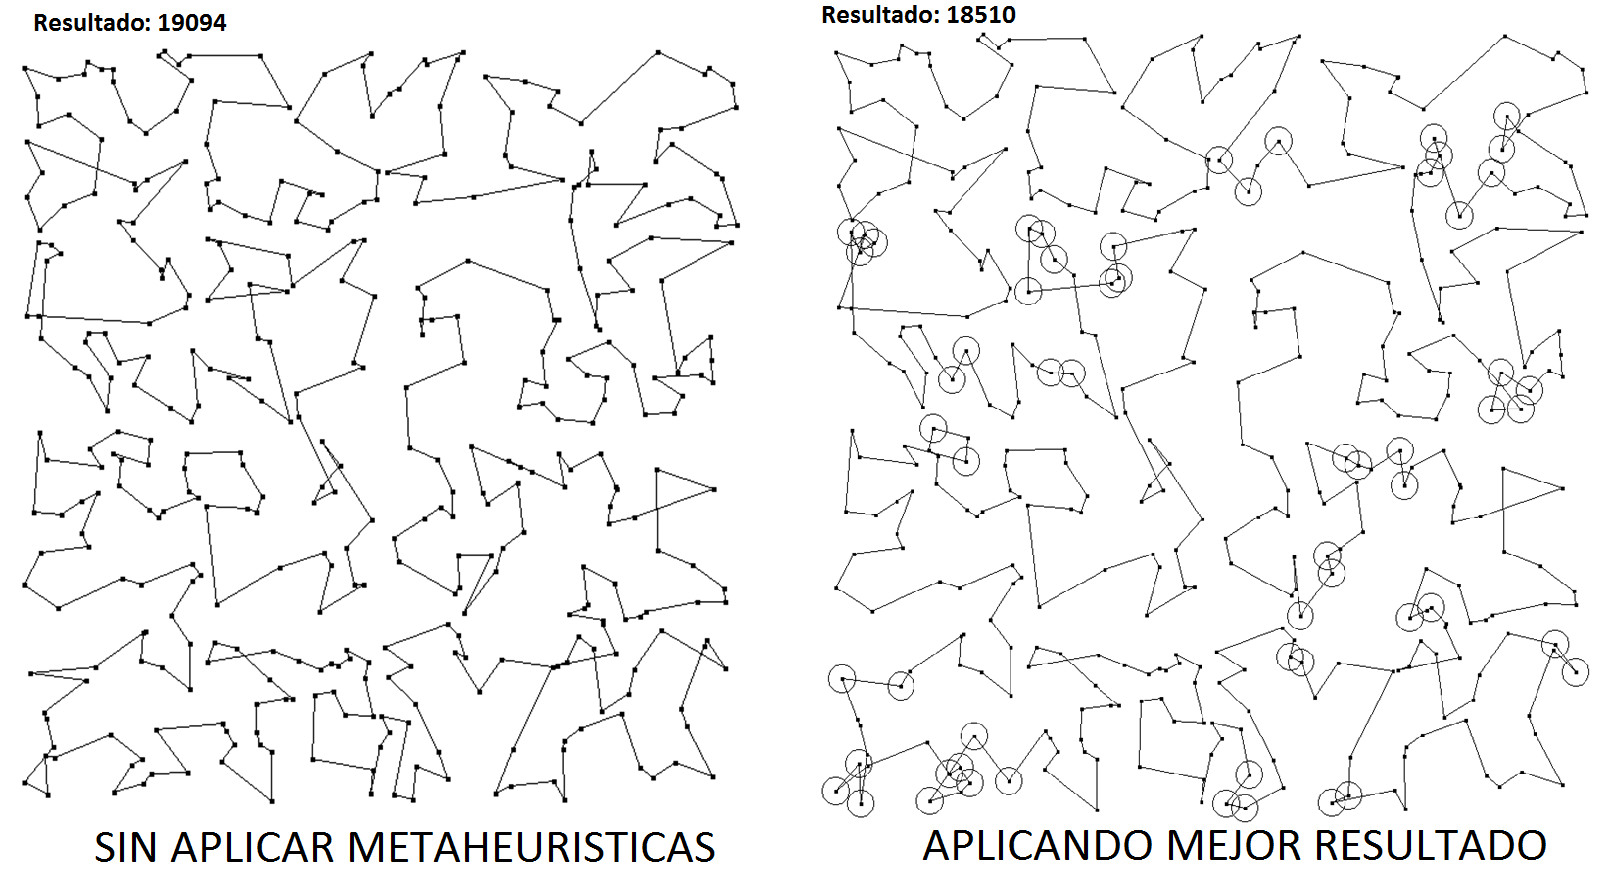
\includegraphics[width=1\textwidth]{PruebasResultados/Experimentos_Comparativas/rd400.png}
        \caption{Comparativa rd400.tsp.}
        \label{fig:rd400_comparativa.png}
\end{figure}
 \begin{figure}[hbtp]
    \centering
        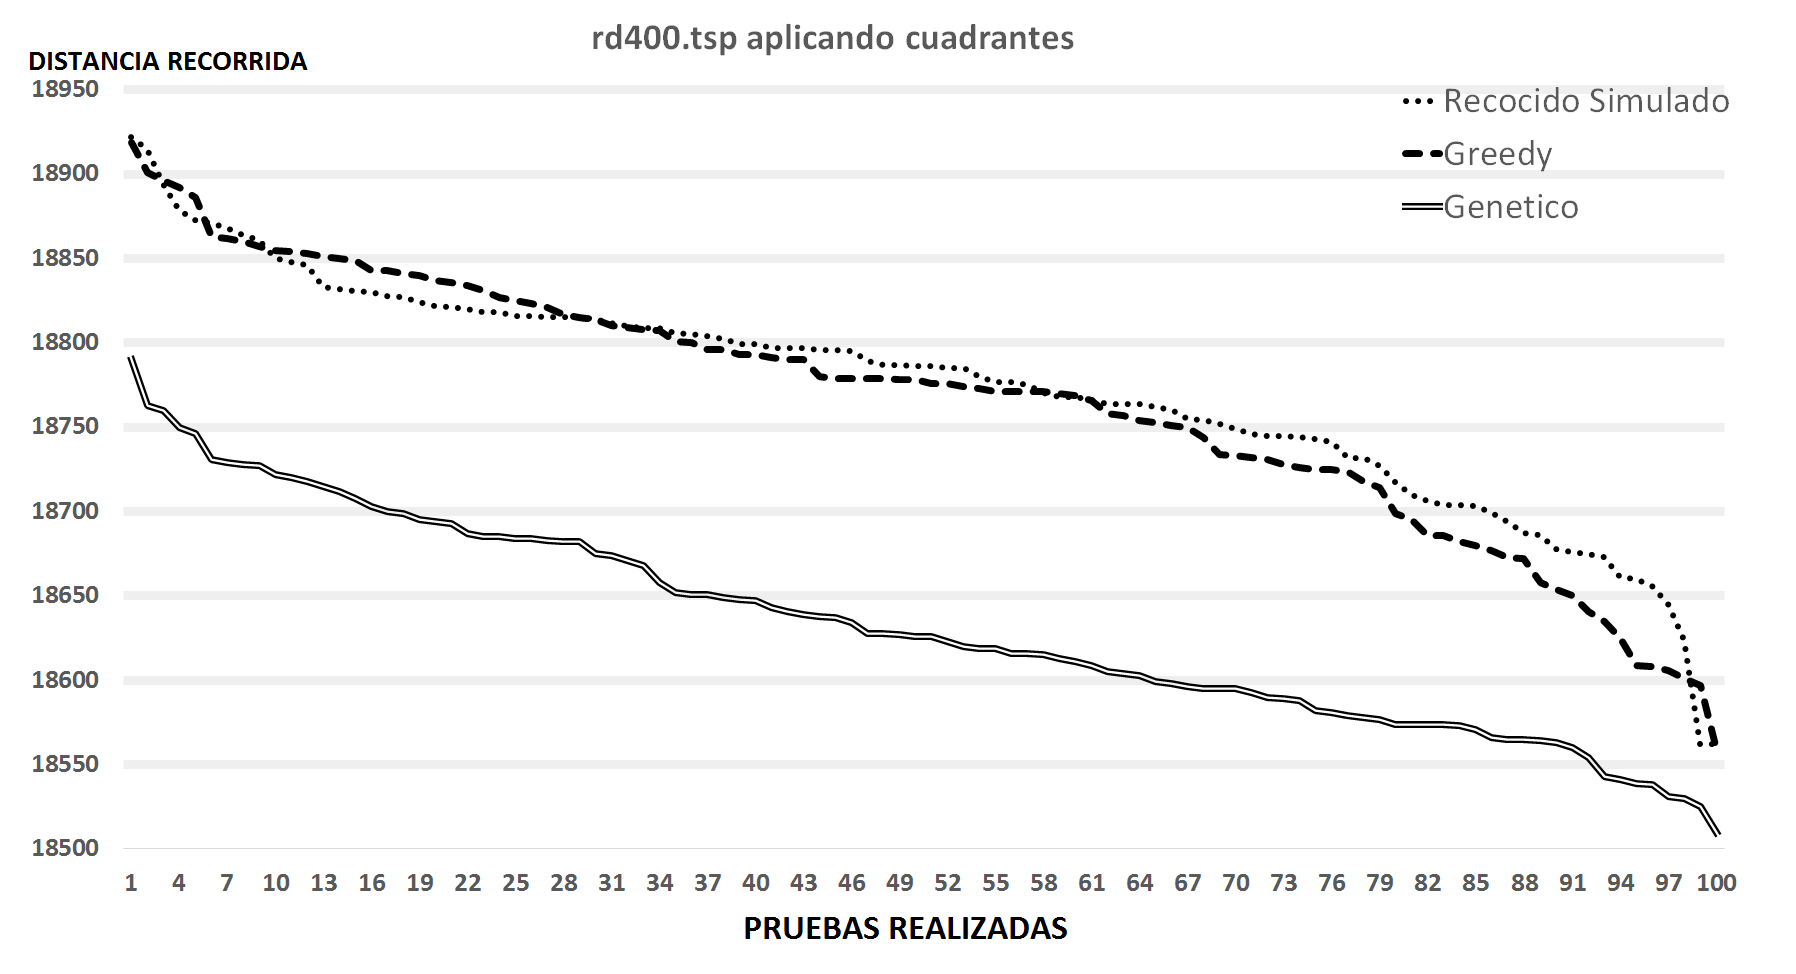
\includegraphics[width=1\textwidth]{PruebasResultados/Experimentos_Graficos_Con/rd400.png}
        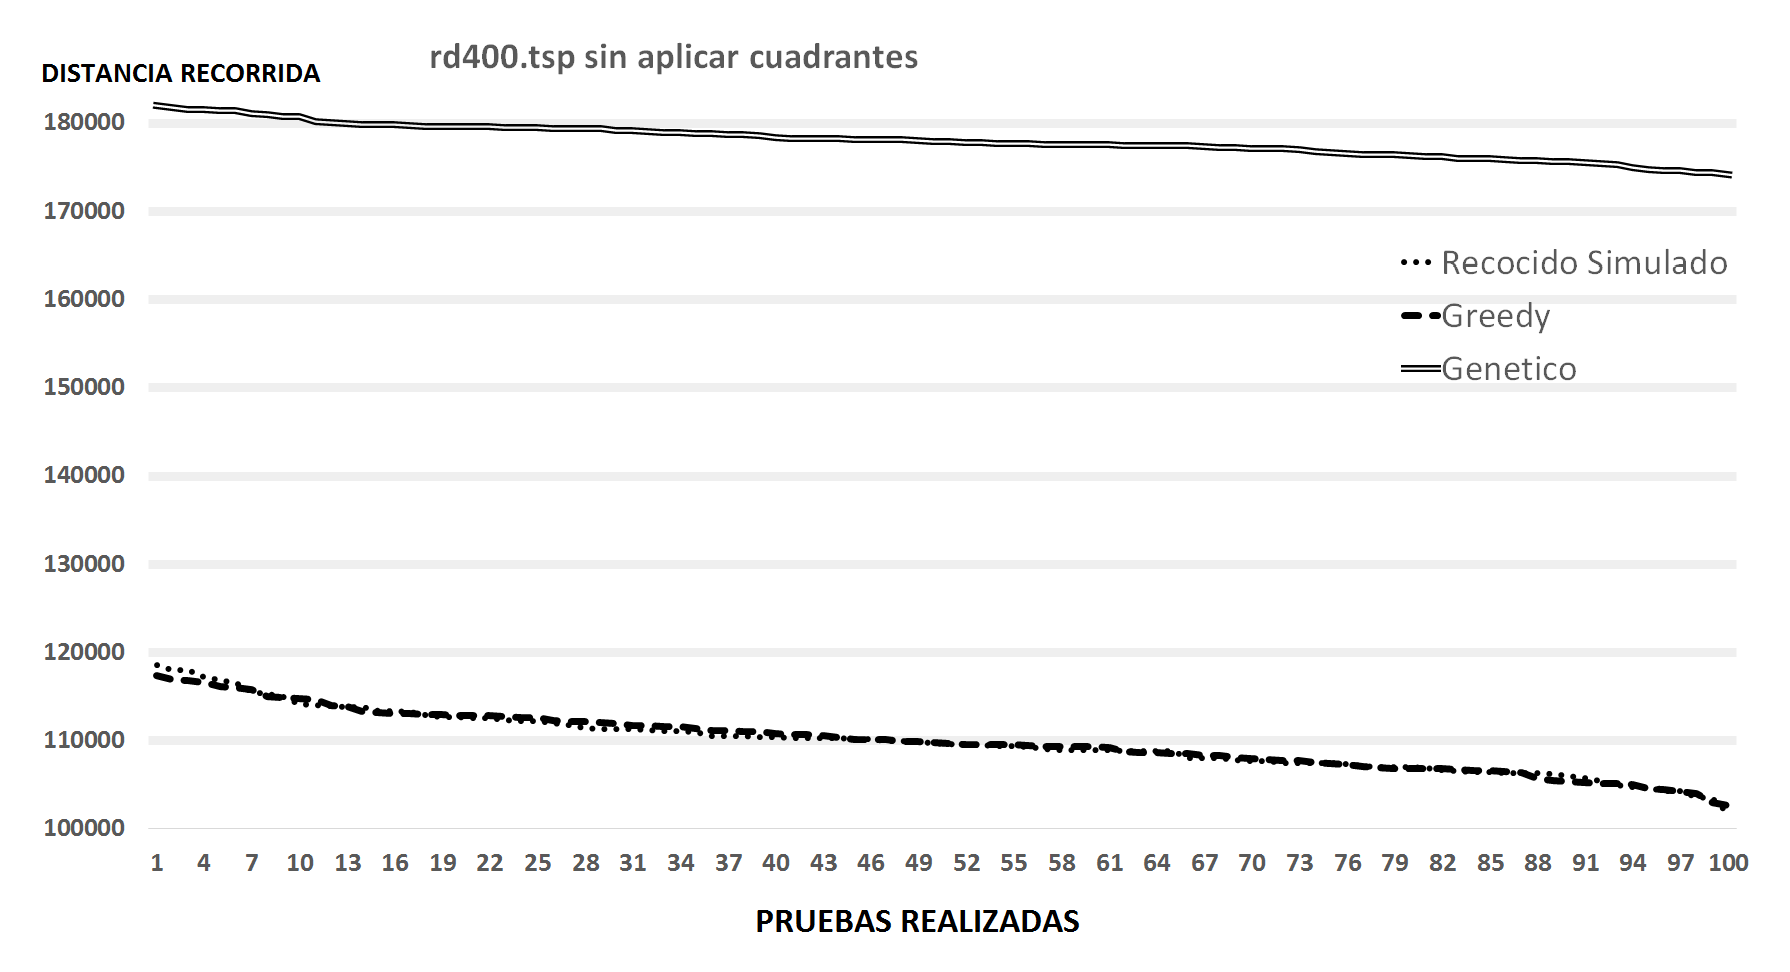
\includegraphics[width=1\textwidth]{PruebasResultados/Experimentos_Graficos_Sin/rd400.png}
        \caption{Gráficos rd400.tsp con cuadrantes y sin cuadrantes.}
        \label{fig:rd400_grafica.png}
\end{figure}
\newpage

%rl5934.TSP
\subsubsection{rl5934.TSP}
\begin{table}[hbtp]
 \centering 
    \caption{Experimento con el problema rl5934.tsp.} 
	\begin{tabular}{ | l   l | r | r | r |   }
         \hline\multicolumn{5}{|c|}{ \rowcolor[gray]{0.8}rl5934.tsp} \\\hline
         \multicolumn{2}{|l|}{Resultado Original :785540}  & Promedio & Mejor & Peor \\ \hline
                & Recocido  & 774838.4 & 772530 & \cellcolor[gray]{0.9} 777479  \\ 
 Con cuadrantes & Greedy    & \cellcolor[gray]{0.9} 774761.73 & \cellcolor[gray]{0.9} 772083 & 778205  \\ 
                & Genético  & 777549.96 & 776338 & 779039  \\ 
                \hline
                & Recocido  & 9349554.00 & \cellcolor[gray]{0.9} 9184381 & \cellcolor[gray]{0.9} 9492444   \\ 
 Sin cuadrantes & Greedy    & \cellcolor[gray]{0.9} 9348025.21 & 9240374 & 9497166   \\ 
                & Genético  & 10249756.12 & 10213188 & 10282877   \\ 
                \hline
    \end{tabular}
    \label{table:EXP_rl5934.tsp}
\end{table}
\begin{figure}[hbtp]
    \centering
        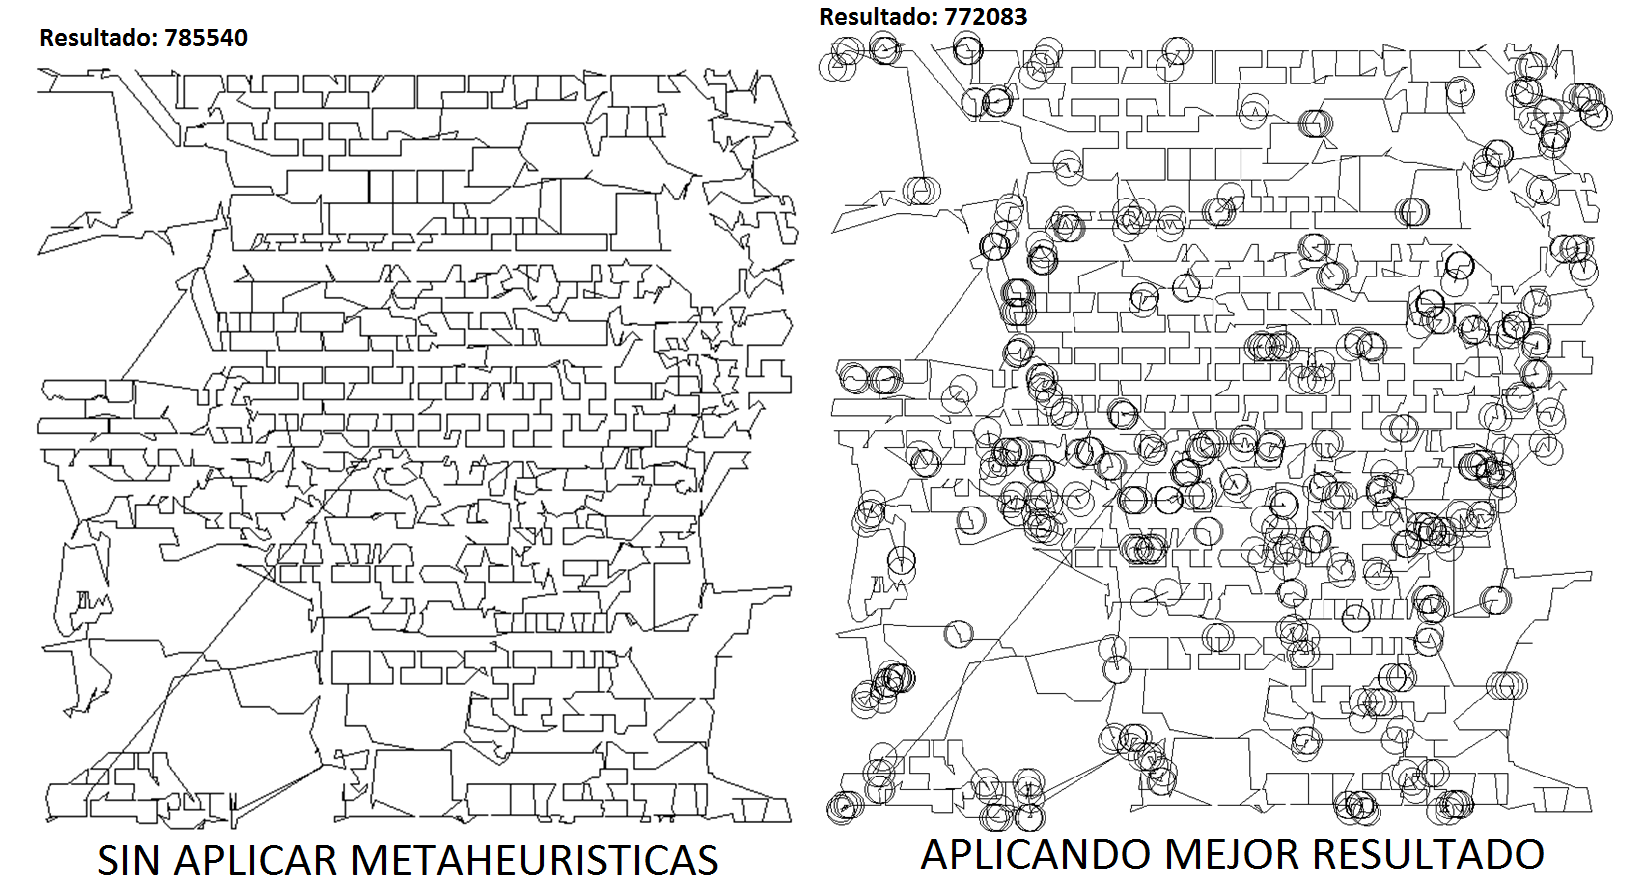
\includegraphics[width=1\textwidth]{PruebasResultados/Experimentos_Comparativas/rl5934.png}
        \caption{Comparativa rl5934.tsp.}
        \label{fig:rl5934_comparativa.png}
\end{figure}
 \begin{figure}[hbtp]
    \centering
        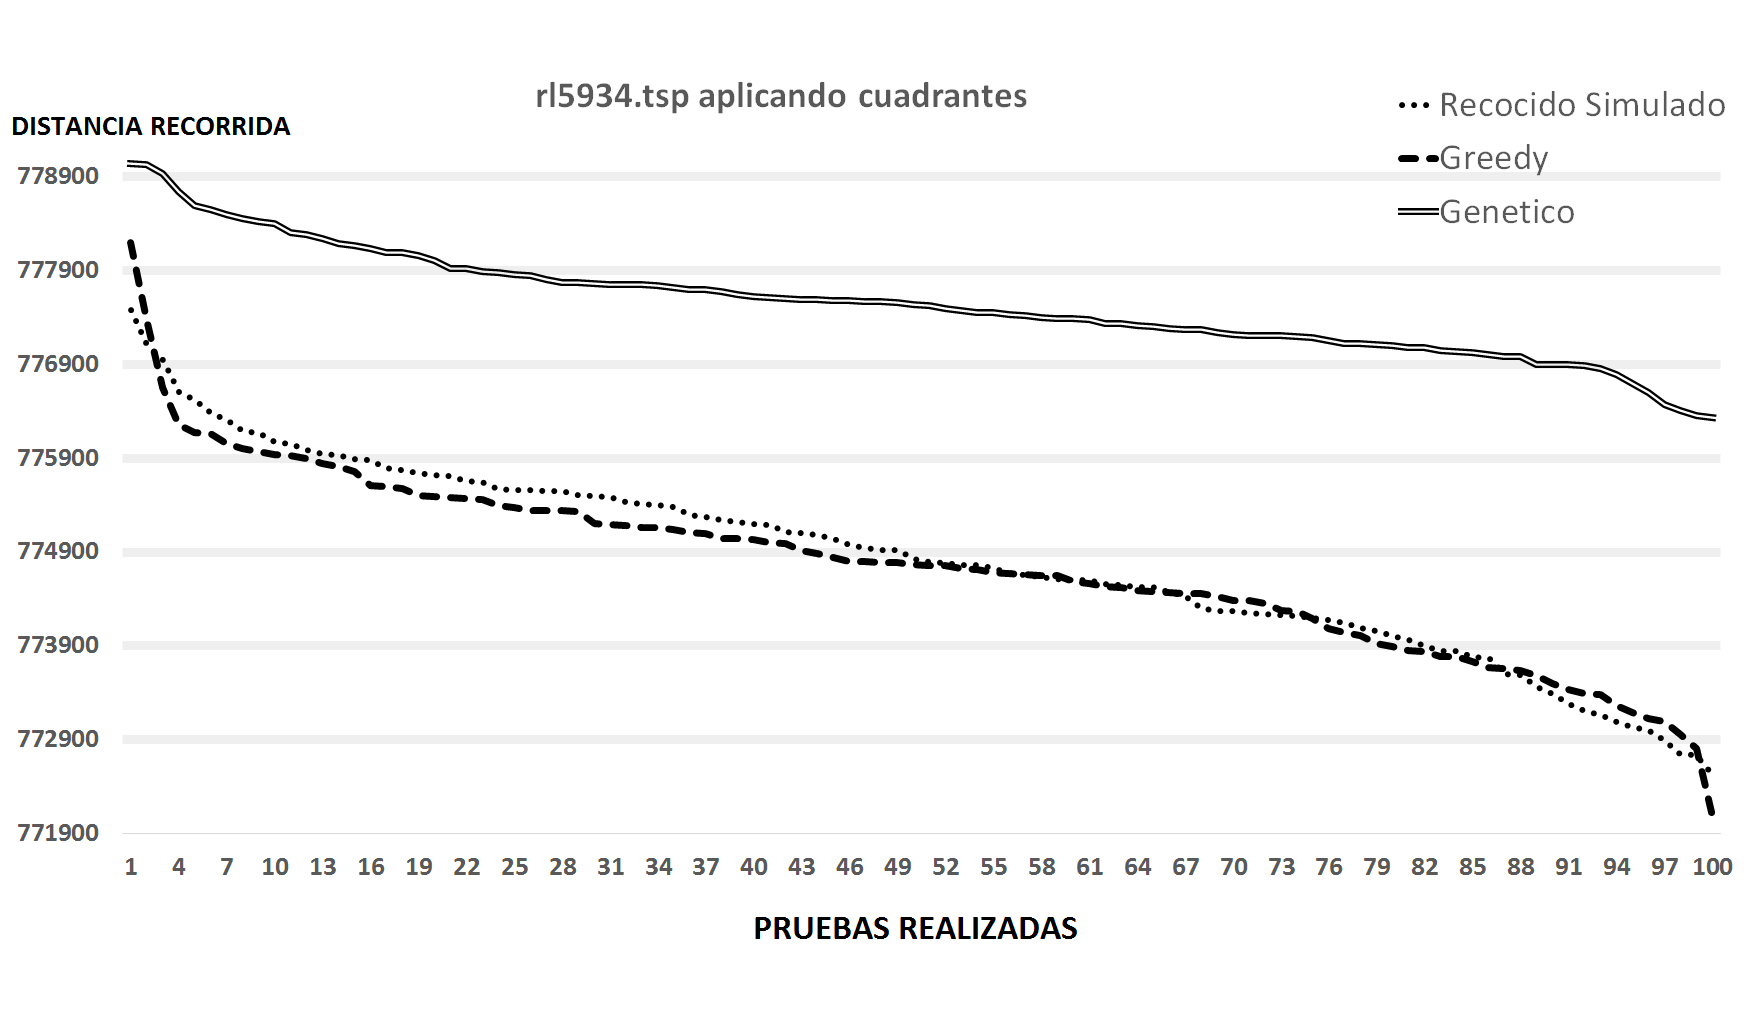
\includegraphics[width=1\textwidth]{PruebasResultados/Experimentos_Graficos_Con/rl5934.png}
        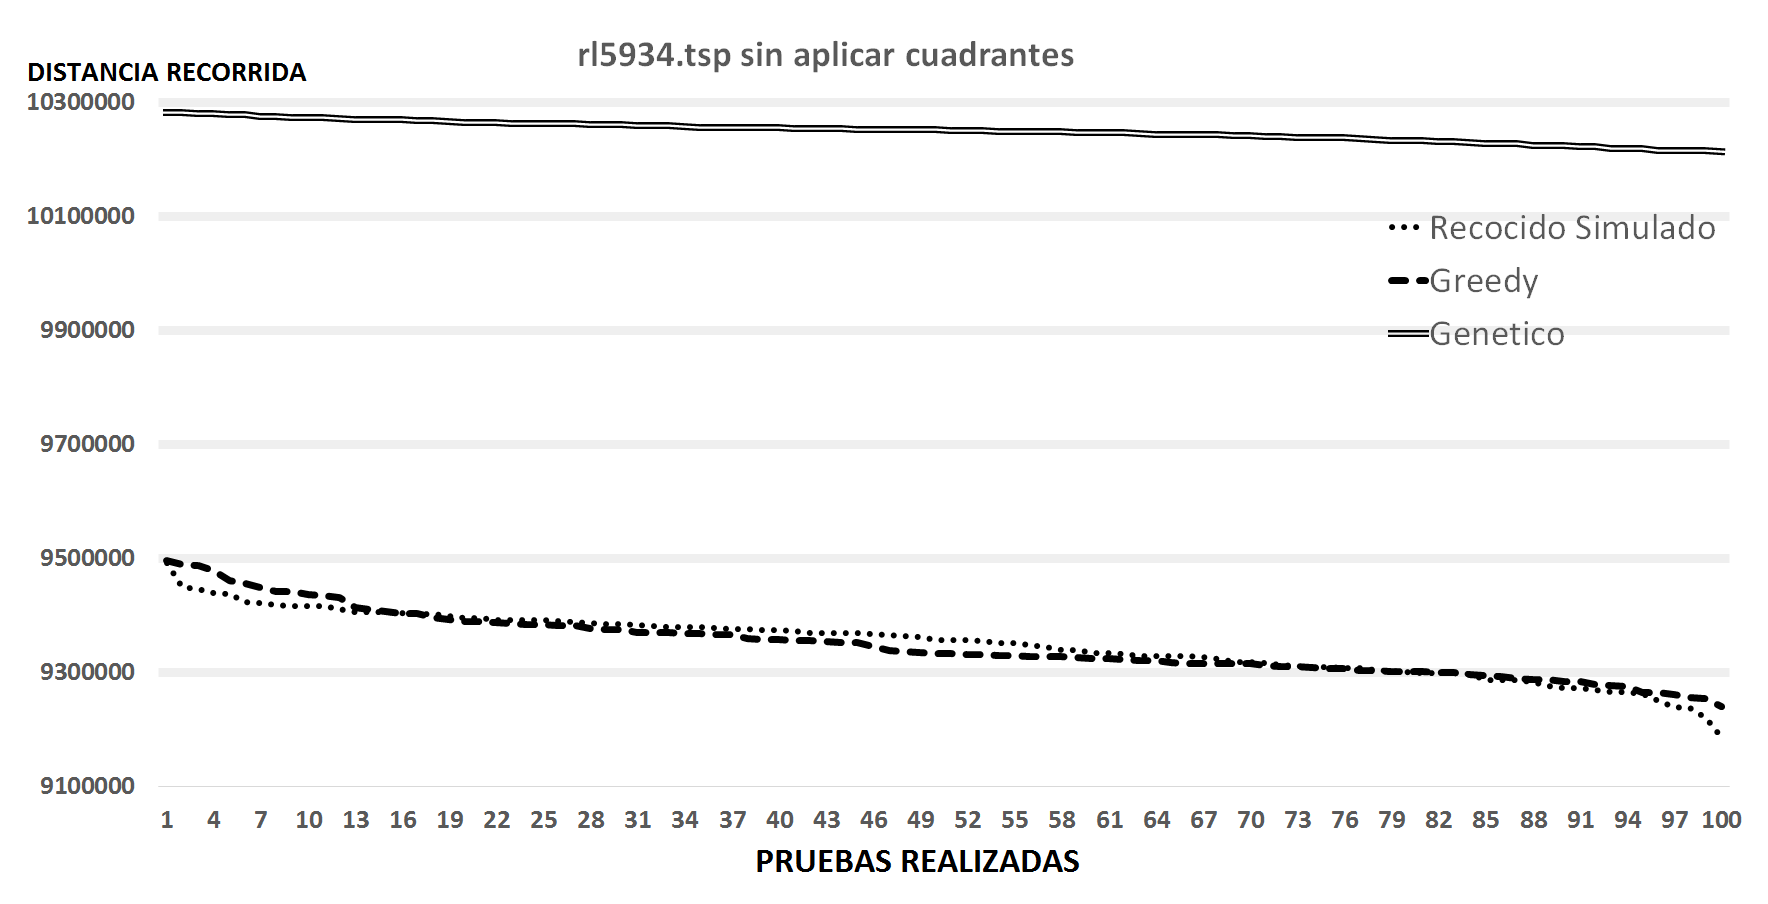
\includegraphics[width=1\textwidth]{PruebasResultados/Experimentos_Graficos_Sin/rl5934.png}
        \caption{Gráficos rl5934.tsp con cuadrantes y sin cuadrantes.}
        \label{fig:rl5934_grafica.png}
\end{figure}
\newpage
%U159.TSP
\subsubsection{u159.TSP}
\begin{table}[hbtp]
 \centering 
    \caption{Experimento con el problema u159.tsp.} 
	\begin{tabular}{ | l   l | r | r | r |   }
       \hline\multicolumn{5}{|c|}{ \rowcolor[gray]{0.8}u159.tsp} \\\hline
         \multicolumn{2}{|l|}{Resultado Original : 56495} & Promedio & Mejor & Peor \\ \hline
                & Recocido  & 55506.95 & 54737 & 56021 \\ 
 Con cuadrantes & Greedy    & 55525.77 & 54992 & 56004 \\ 
                & Genético  & \cellcolor[gray]{0.9} 54834.24 & \cellcolor[gray]{0.9} 54418 & \cellcolor[gray]{0.9} 55238 \\ \hline
                & Recocido  & 68629.83 & 65324 & 74869 \\ 
 Sin cuadrantes & Greedy    & 68829.22 & 65058 & 73971 \\ 
                & Genético  & \cellcolor[gray]{0.9} 62582.97 & \cellcolor[gray]{0.9} 59906 & \cellcolor[gray]{0.9} 65035 \\ 
                \hline
    \end{tabular}
    \label{table:EXP_u159.tsp}
\end{table}
\begin{figure}[hbtp]
    \centering
        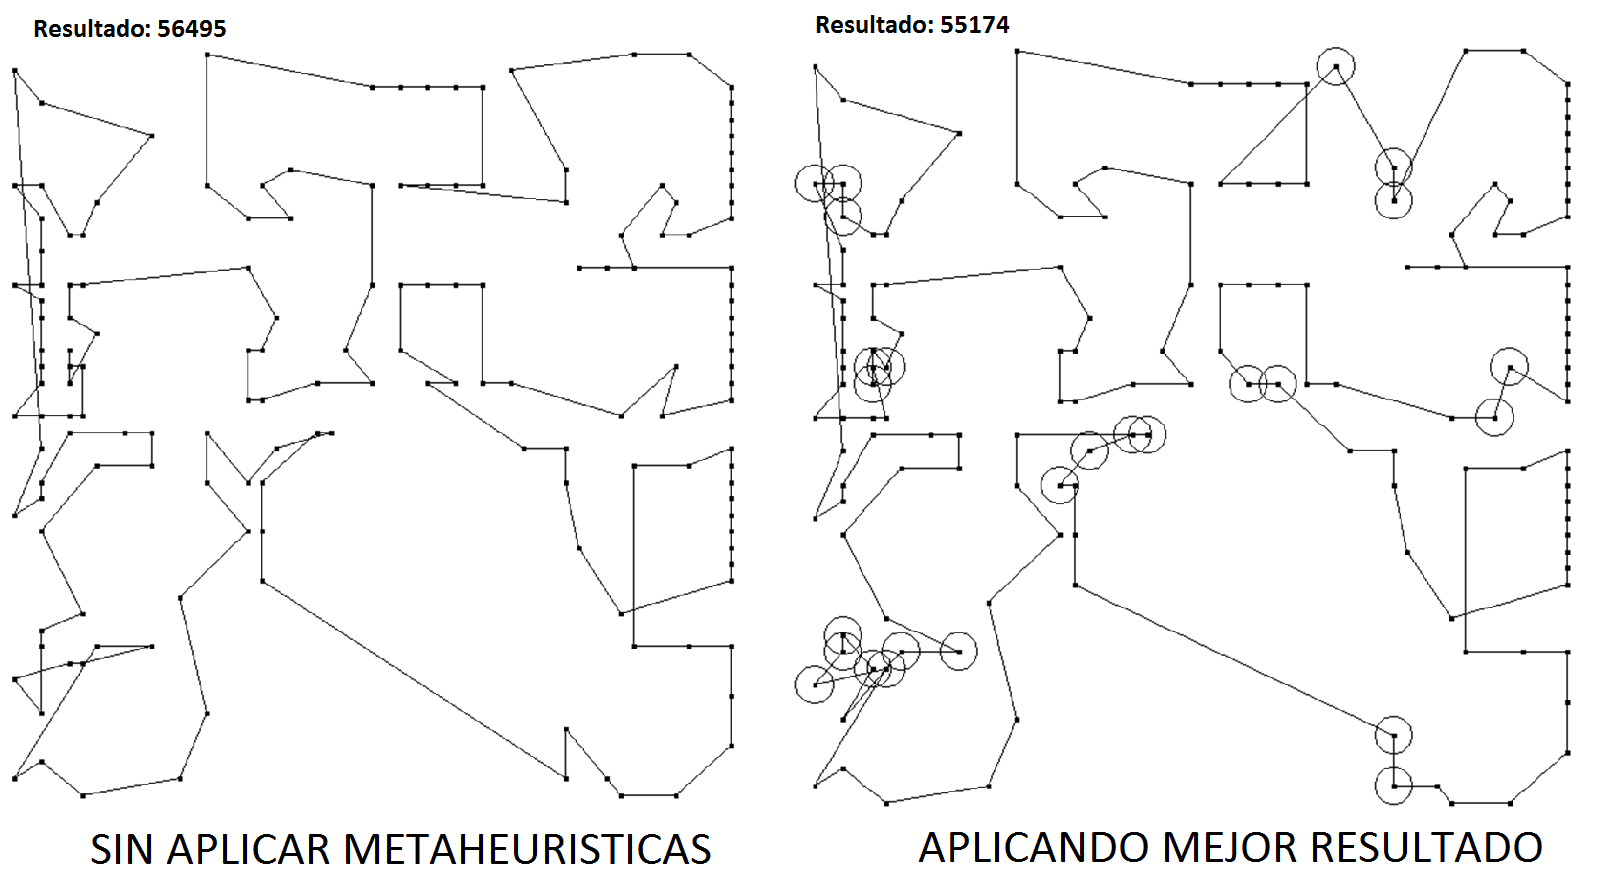
\includegraphics[width=1\textwidth]{PruebasResultados/Experimentos_Comparativas/u159.png}
        \caption{Comparativa u159.tsp.}
        \label{fig:u159_comparativa.png}
\end{figure}
 \begin{figure}[hbtp]
    \centering
        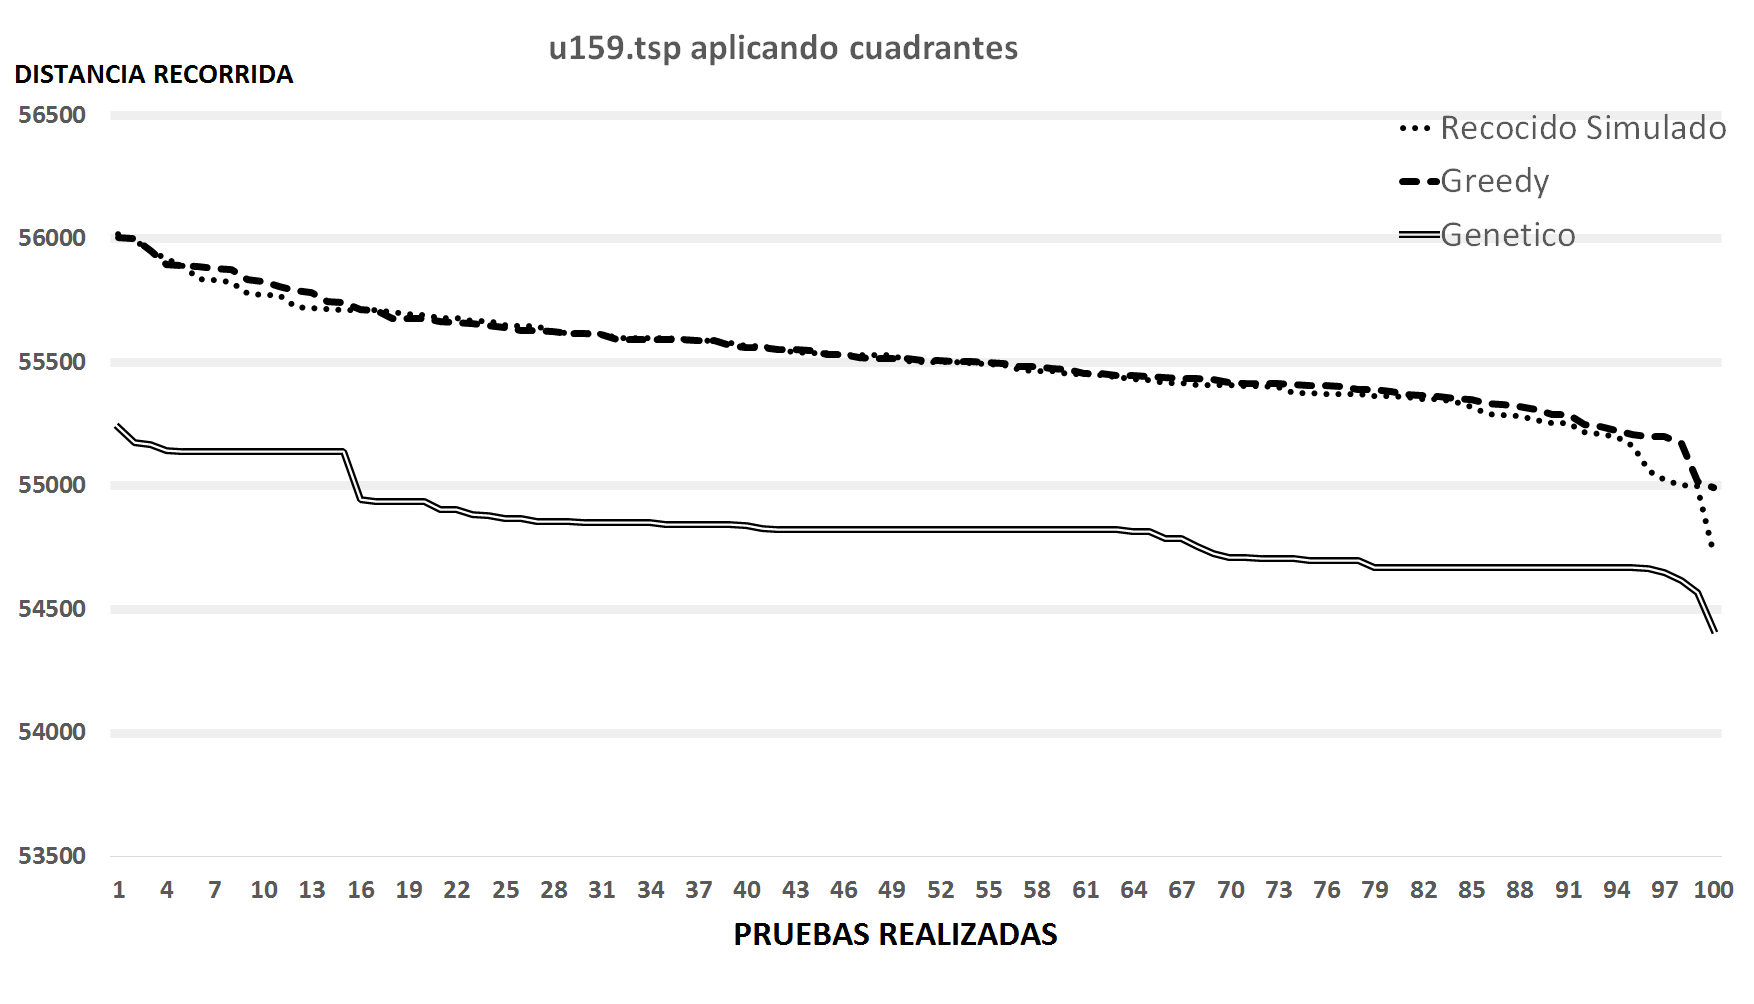
\includegraphics[width=1\textwidth]{PruebasResultados/Experimentos_Graficos_Con/u159.png}
        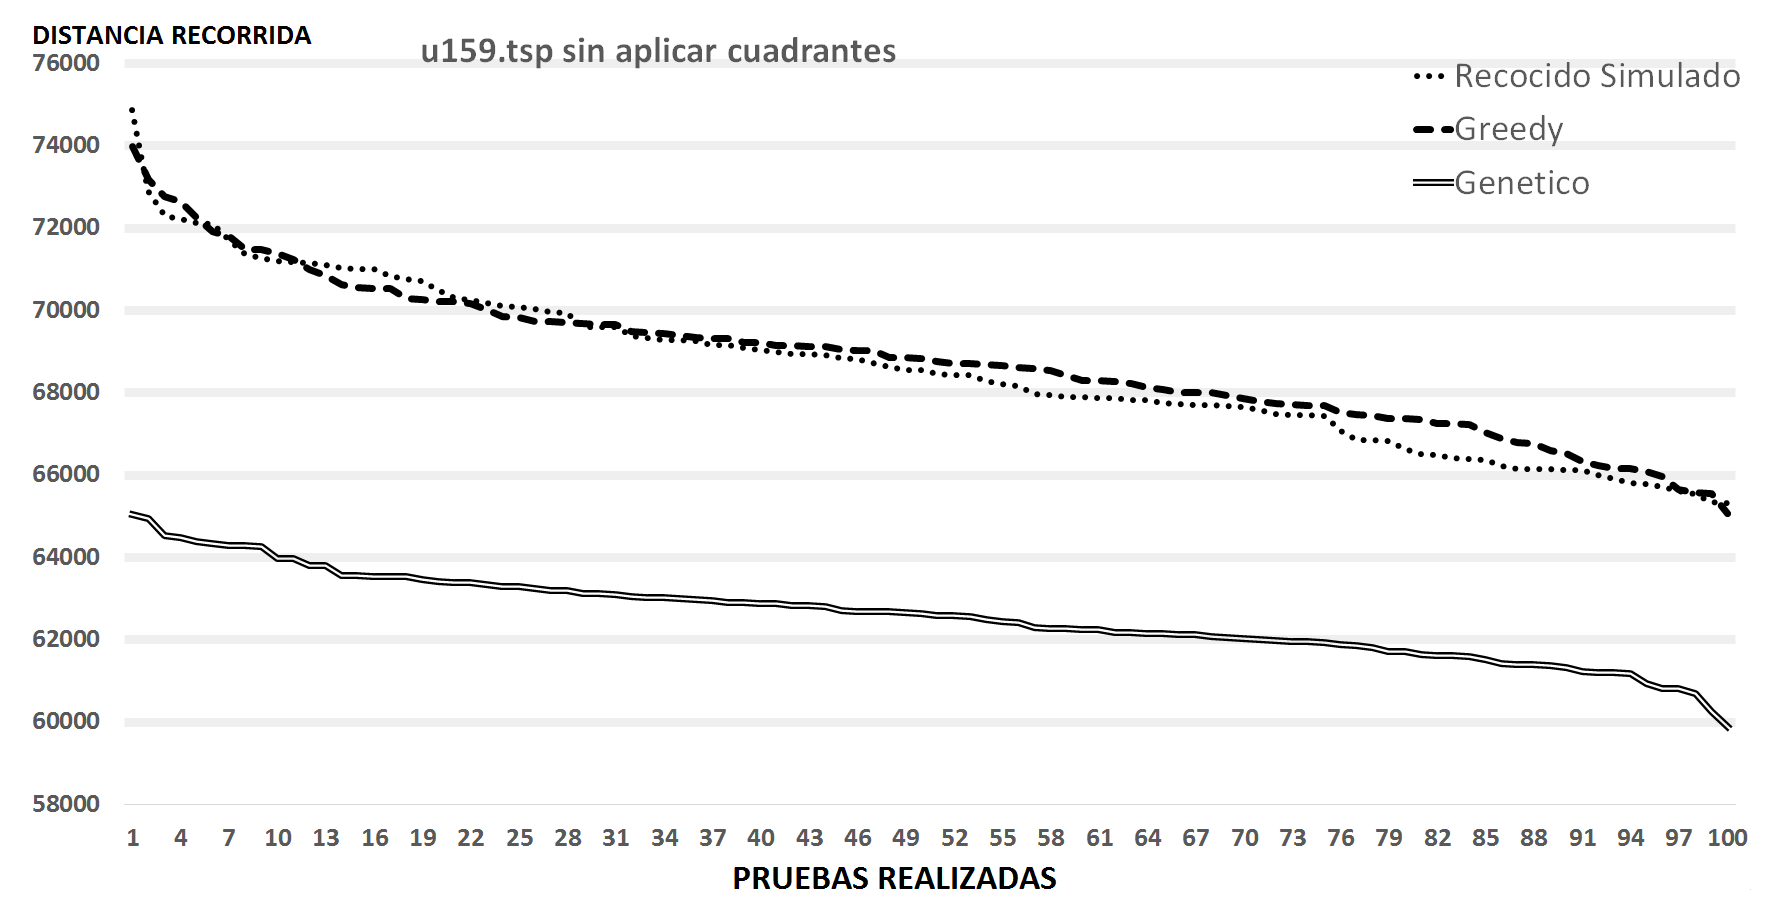
\includegraphics[width=1\textwidth]{PruebasResultados/Experimentos_Graficos_Sin/u159.png}
        \caption{Gráficos u159.tsp con cuadrantes y sin cuadrantes.}
        \label{fig:u159_grafica.png}
\end{figure}
\newpage

%u724.TSP
\subsubsection{u724.TSP}
\begin{table}[hbtp]
 \centering 
    \caption{Experimento con el problema u724.tsp.}
	\begin{tabular}{ | l   l | r | r | r |   }
         \hline \multicolumn{5}{|c|}{ \rowcolor[gray]{0.8}u724.tsp } \\\hline
         \multicolumn{2}{|l|}{Resultado Original : 57641} & Promedio & Mejor & Peor \\ \hline
                & Recocido  & 55976.89 & 55514 & 56479  \\ 
 Con cuadrantes & Greedy    & 56010.58 & 55474 & 56725  \\ 
                & Genético  & \cellcolor[gray]{0.9} 55004.45 & \cellcolor[gray]{0.9} 54685 & \cellcolor[gray]{0.9} 55283 \\ \hline
                & Recocido  & 140950.10 & 134129 & 149630   \\ 
 Sin cuadrantes & Greedy    & \cellcolor[gray]{0.9} 140872.24 & \cellcolor[gray]{0.9} 132686 & \cellcolor[gray]{0.9} 149355 \\ 
                & Genético  & 168973.59 & 164770 & 171946   \\ 
                \hline
    \end{tabular}
    \label{table:EXP_u724.tsp}
\end{table}	
\begin{figure}[hbtp]
    \centering
        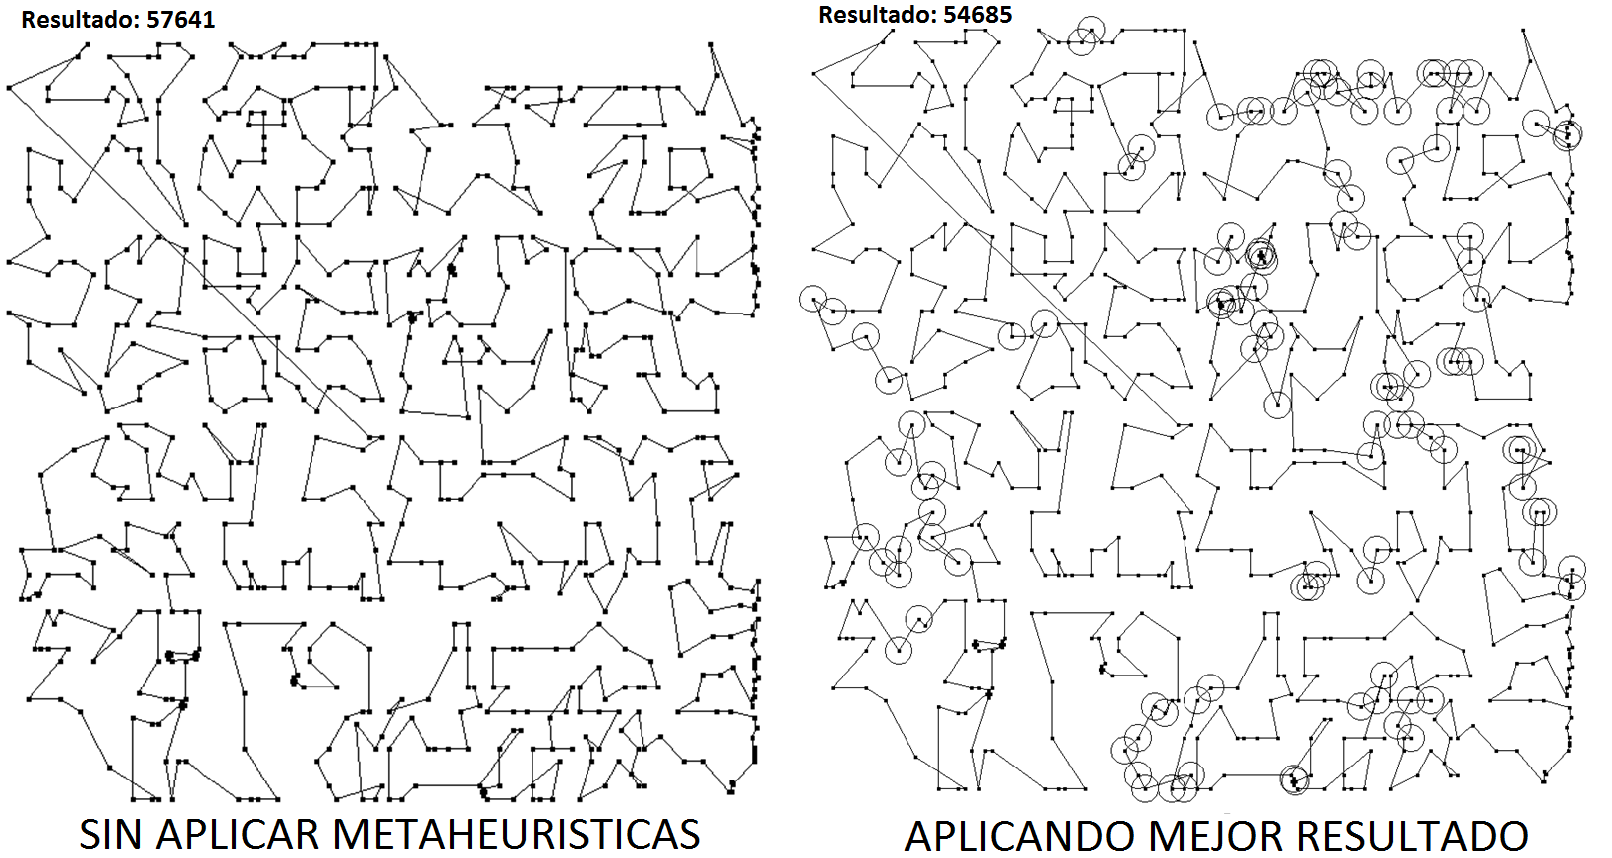
\includegraphics[width=1\textwidth]{PruebasResultados/Experimentos_Comparativas/u724.png}
        \caption{Comparativa u724.tsp.}
        \label{fig:u724_comparativa.png}
\end{figure}
 \begin{figure}[hbtp]
    \centering
        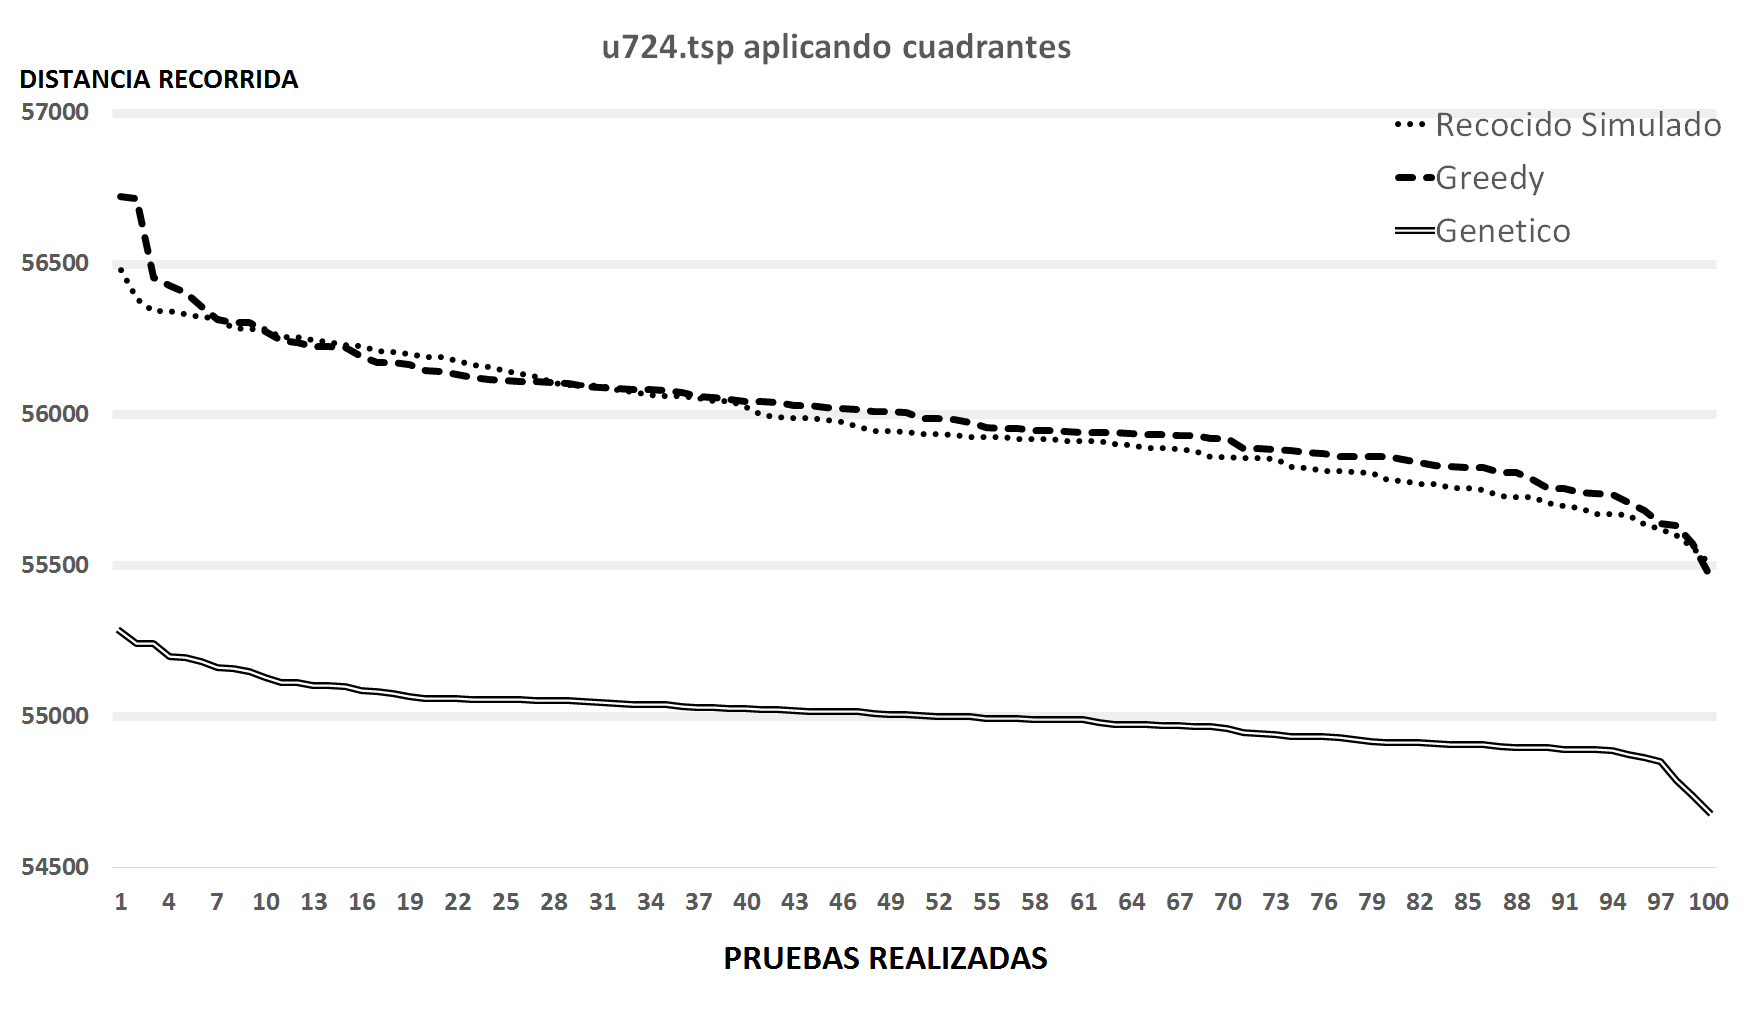
\includegraphics[width=1\textwidth]{PruebasResultados/Experimentos_Graficos_Con/u724.png}
        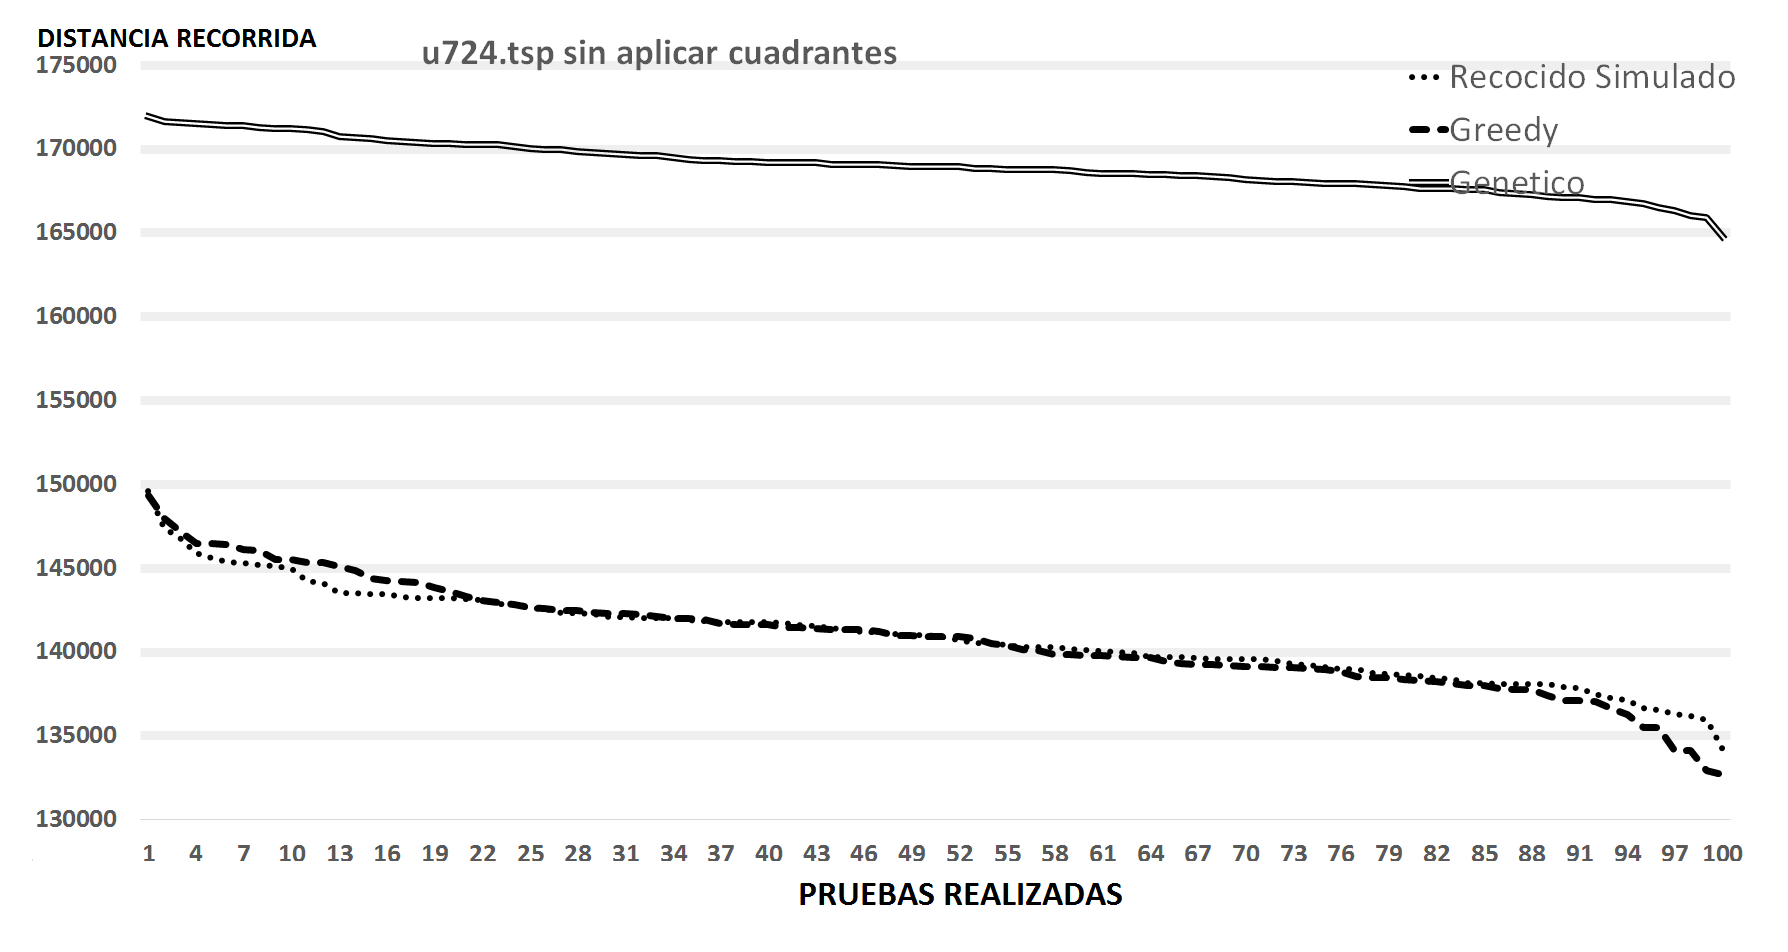
\includegraphics[width=1\textwidth]{PruebasResultados/Experimentos_Graficos_Sin/u724.png}
        \caption{Gráficos u724.tsp con cuadrantes y sin cuadrantes.}
        \label{fig:u724_grafica.png}
\end{figure}
\newpage

%vm1084.TSP
\subsubsection{vm1084.TSP}
\begin{table}[hbtp]
 \centering 
    \caption{Experimento con el problema vm1084.tsp.} 
	\begin{tabular}{ | l   l | r | r | r |   }
         \hline \multicolumn{5}{|c|}{ \rowcolor[gray]{0.8}vm1084.tsp} \\\hline
         \multicolumn{2}{|l|}{Resultado Original :344972}  & Promedio & Mejor & Peor \\ \hline
                & Recocido  & 334821.39 & 330999 & 338557 \\ 
 Con cuadrantes & Greedy    & 335133.04 & 331589 & 339023 \\ 
                & Genético  & \cellcolor[gray]{0.9} 331384.21 & \cellcolor[gray]{0.9} 329200 & \cellcolor[gray]{0.9} 333749 \\ 
                \hline
                & Recocido  & 3224207.18 & 3064309 & 3380496 \\ 
 Sin cuadrantes & Greedy    & \cellcolor[gray]{0.9} 3214476.72 & \cellcolor[gray]{0.9} 3063644 & \cellcolor[gray]{0.9} 3363287\\
                & Genético  & 4772212.30 & 4671155 & 4850260 \\ 
                \hline
    \end{tabular}
    \label{table:EXP_vm1084.tsp}
\end{table}
\begin{figure}[hbtp]
    \centering
        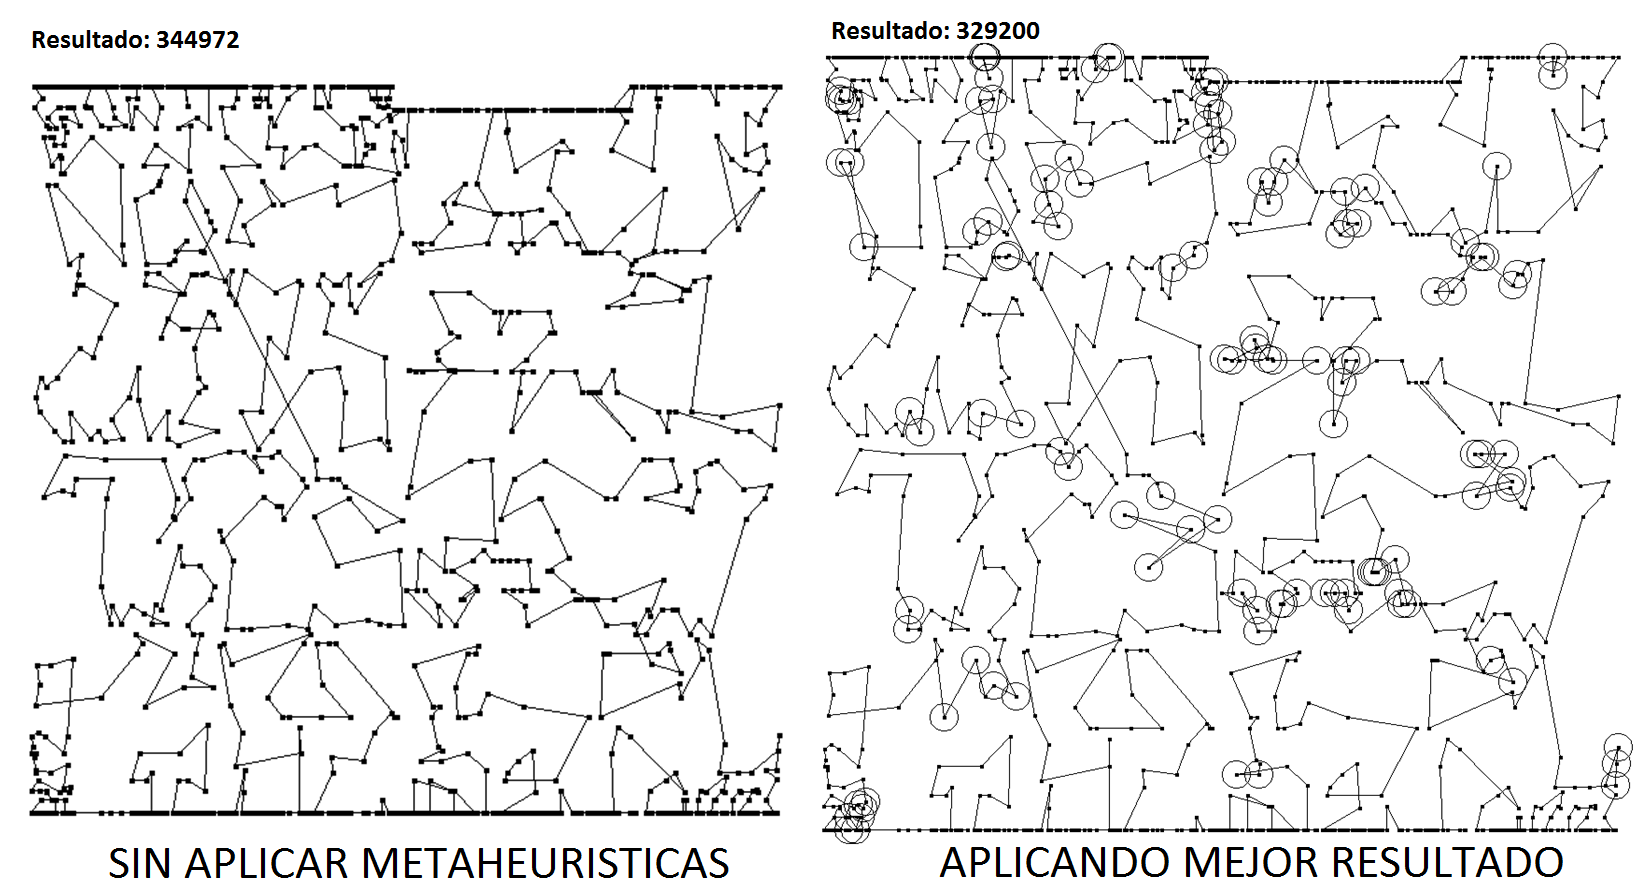
\includegraphics[width=1\textwidth]{PruebasResultados/Experimentos_Comparativas/vm1084.png}
        \caption{Comparativa vm1084.tsp.}
        \label{fig:vm1084_comparativa.png}
\end{figure}
 \begin{figure}[hbtp]
    \centering
        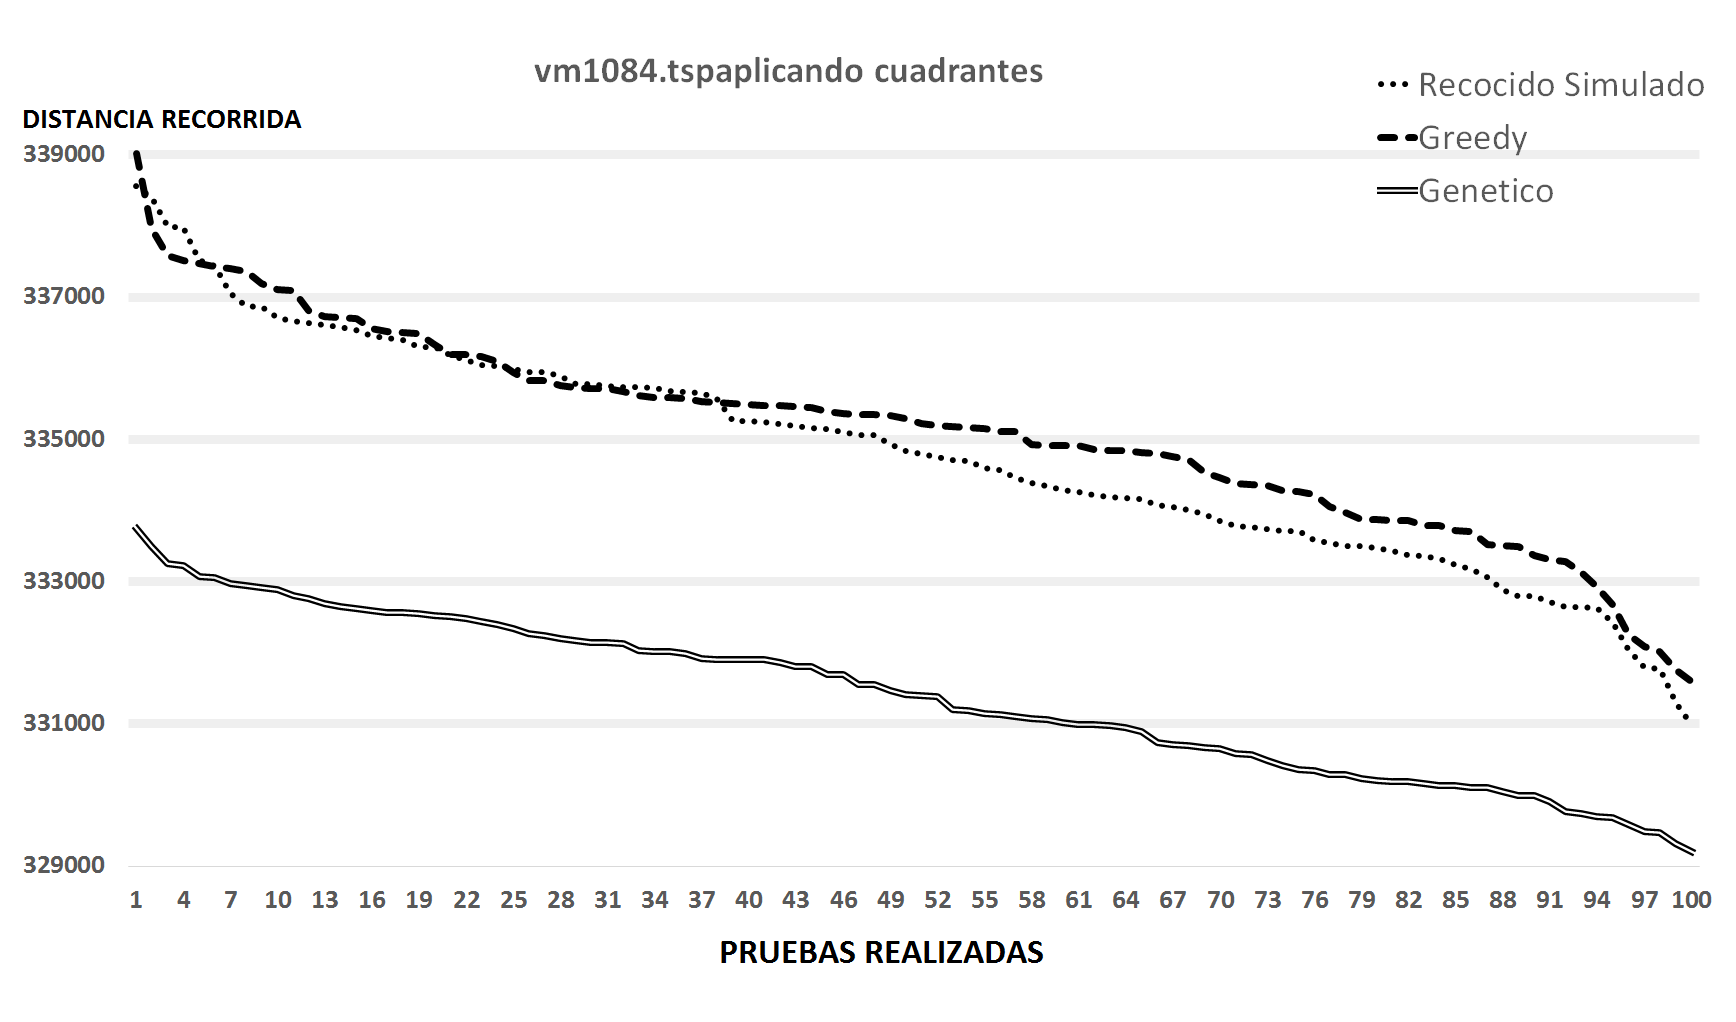
\includegraphics[width=1\textwidth]{PruebasResultados/Experimentos_Graficos_Con/vm1084.png}
        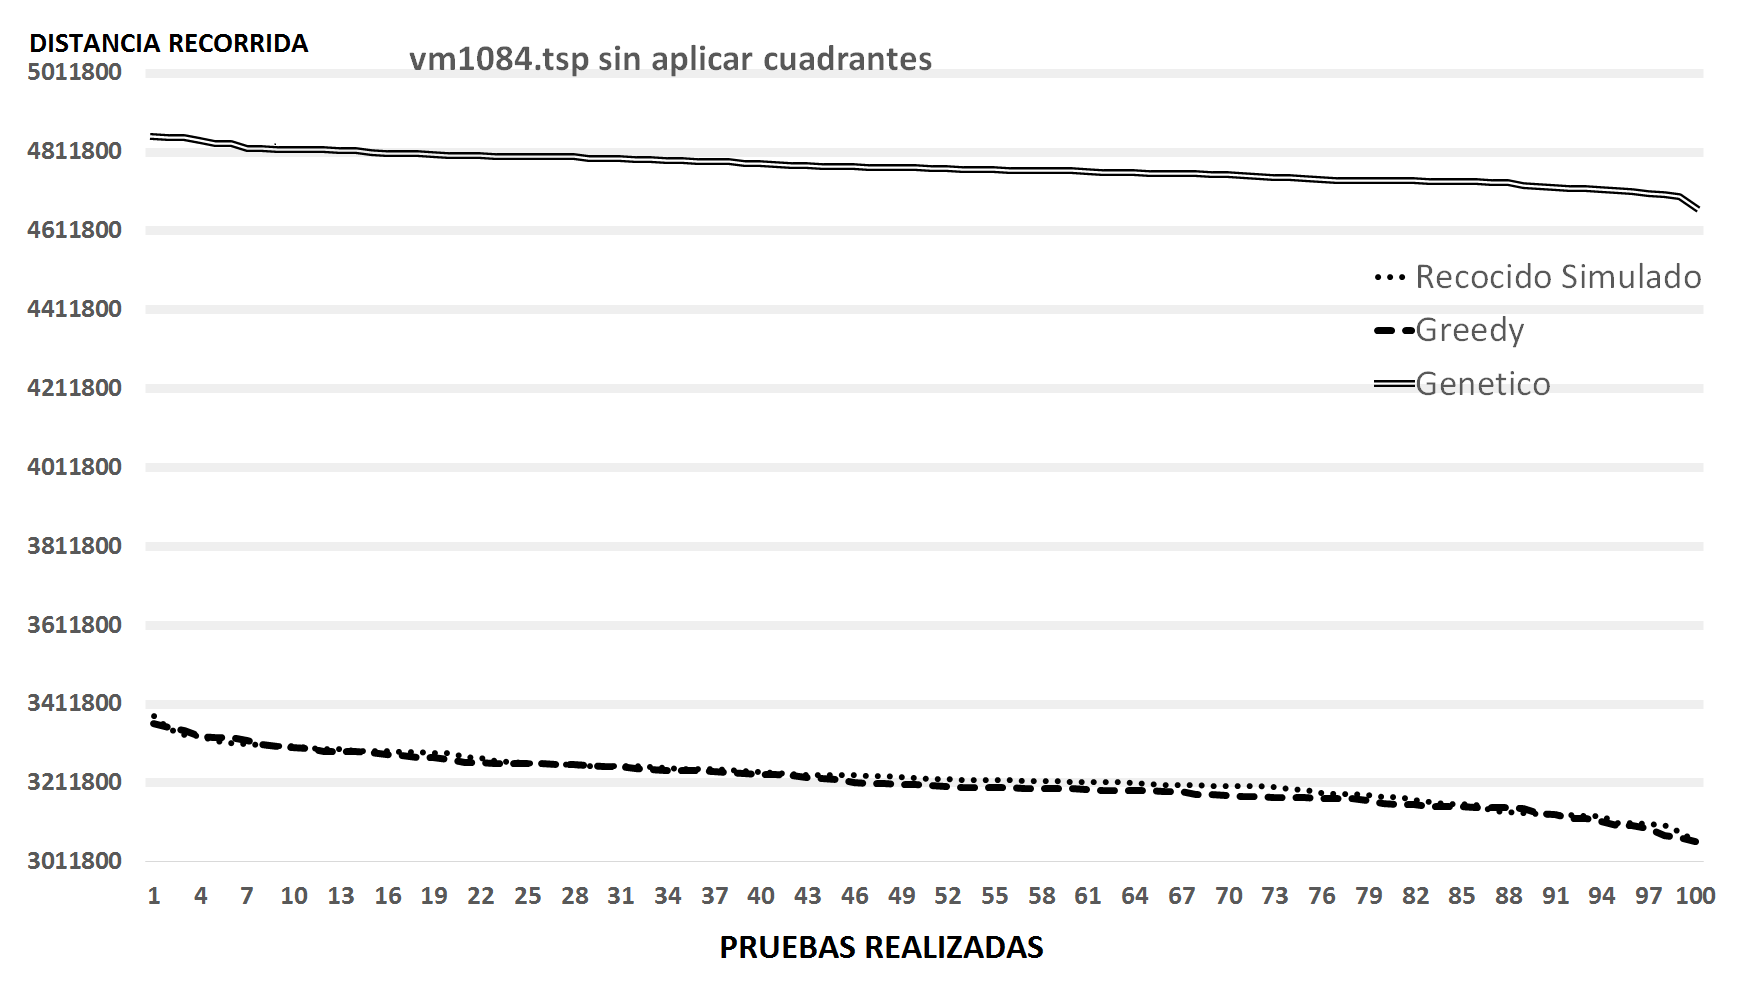
\includegraphics[width=1\textwidth]{PruebasResultados/Experimentos_Graficos_Sin/vm1084.png}
        \caption{Gráficos vm1084.tsp con cuadrantes y sin cuadrantes.}
        \label{fig:vm1084_grafica.png}
\end{figure}
\newpage

 %\begin{figure}[hbtp]
    %\centering
       
     %   \caption{Grafico a280.tsp sin cuadrantes.}
      %  \label{fig:a280_comparativa.png}
%\end{figure}

    
